\documentclass[12pt,a4paper]{report}

% =======================
% Packages
% =======================
\usepackage[utf8]{inputenc}
\usepackage[T1]{fontenc}
\usepackage[french]{babel}
\usepackage{lmodern}
\usepackage{geometry}
\geometry{margin=2.5cm}
\usepackage{graphicx}
\usepackage{booktabs}
\usepackage{hyperref}
\usepackage{float}
\usepackage{enumitem}
\usepackage{titlesec}
\usepackage{amsmath}
\usepackage{amssymb}
\usepackage{setspace}
\usepackage{caption}
\usepackage{pdflscape}

\setstretch{1.15} % Interligne légèrement augmenté pour une bonne lisibilité

\hypersetup{colorlinks=true, linkcolor=blue, urlcolor=blue, citecolor=black}

\setcounter{tocdepth}{3}

\begin{document}

% =======================
% Page de couverture
% =======================
\begin{titlepage}
    \centering
    \vspace*{1.2cm}

    
\includegraphics[width=0.22\textwidth]{figures/logo_ensae.pdf}\par
    \vspace{0.8cm}
    
    {\scshape\LARGE ENSAE Paris \par}
    \vspace{1cm}
    {\scshape\Large Projet Stat'App \par}
    \vspace{1.5cm}
    
    \rule{\linewidth}{0.5mm} \\[0.4cm]
    {\huge \bfseries Unsupervised \& Semi‑Supervised Product Categorization at Scale into the Google Product Taxonomy \par}
    \vspace{0.4cm}
    \rule{\linewidth}{0.5mm} \\[1.5cm]
    
    \Large
    \emph{Auteurs :}\\
    Salah Eddine NEJJARI, Tao DANG TRAN, \\
    Thomas FAVRE, Yohan ANDRIAMAMPIONONA\par
    
    \vspace{1cm}
    \normalsize
    \emph{Sous le tutorat de :} \\
    Guillaume Lochon (Critéo)\\
    Ilan Benchetrit (Critéo)\\ 
    Nicolas Chopin (Ensae)\\
    
    \vfill
    {\large Mai 2026 \par}
\end{titlepage}

% =======================
% Sommaire
% =======================
\tableofcontents
\newpage

% =======================
% 1. Introduction
% =======================
\chapter{Introduction}
\label{chap:introduction}

\section{Objectifs du projet}
Ce projet a été initié par l'entreprise Critéo. Il constitue un exercice pédagogique et n'a pas vocation à être déployé directement en production.
Son objectif est de construire un pipeline de classification hiérarchique de produits à partir d'un catalogue partiellement annoté.
Pour cela, nous mobilisons des techniques de NLP (\textit{Natural Language Processing}).

\section{Présentation de l'entreprise Critéo et contextualisation du problème}

Critéo est un acteur mondial de la publicité en ligne, spécialisé dans le ciblage et l'affichage personnalisé de bannières publicitaires pour les entreprises.
Pour comprendre l'importance de la classification des produits, il faut rappeler le mécanisme d'affichage publicitaire. Lorsqu'une bannière peut être affichée, plusieurs acteurs participent à une enchère en temps réel. 
Le gagnant obtient le droit d'afficher sa publicité. Critéo doit donc décider rapidement s'il est pertinent d'enchérir pour afficher une publicité à un utilisateur donné, puis se rémunère notamment à partir des clics sur la bannière publicitaire ou d'autres indicateurs de performance.
Il existe donc un arbitrage permanent entre le coût de l'enchère, la probabilité que l'utilisateur clique sur la publicité et la valeur attendue de cette interaction.

Au cœur de ce modèle économique se trouve la nécessité de traiter quotidiennement des catalogues de produits massifs et hétérogènes. Pour afficher la bonne publicité au bon consommateur, une compréhension sémantique fine de chaque article est indispensable. Une classification détaillée des produits, avec un taux d'erreur aussi faible que possible, constitue donc une étape importante de l'ensemble du pipeline de Critéo.

\section{Problématisation et méthodologie adoptée}

Le problème posé consiste à classer 128\,000 produits dans une taxonomie extrêmement granulaire : la taxonomie Google, qui comprend plus de 5\,400 catégories réparties sur sept niveaux de profondeur.


Nous disposons donc de deux sources principales :
\begin{itemize}[leftmargin=1.2cm]
    \item une taxonomie hiérarchique, dans laquelle les catégories sont organisées par niveaux. Par exemple, \textit{home \& garden} est une catégorie de Niveau 1 contenant des sous-catégories de Niveau 2 comme \textit{furniture} ou \textit{kitchen \& dining} ;
    \item un catalogue de produits annoté au Niveau 1, c'est-à-dire que chaque produit possède une grande catégorie, mais pas nécessairement sa catégorie fine dans les niveaux profonds.
\end{itemize}

Une contrainte importante fixée par Critéo était de privilégier des solutions à faible coût de calcul et à faible coût d'inférence. Autrement dit, la classification d'un nouveau produit ne doit pas nécessiter une puissance de calcul excessive ni un temps de classification trop élevé. Cette contrainte a guidé le choix d'une architecture fondée sur des modèles d'embeddings compacts : peu de paramètres et une dimension vectorielle réduite, plutôt que des appels répétés à de grands modèles génératifs.

Une limite méthodologique majeure doit toutefois être posée dès l'introduction : la vérité terrain n'est disponible que pour le Niveau 1. Les niveaux L2--L7 ne sont pas annotés de manière exploitable dans les données du projet. Les métriques utilisées pour ces niveaux ne doivent donc pas être interprétées comme une accuracy supervisée ; elles mesurent des coûts, des marges de confiance, des accords entre pipelines et des scores sémantiques indirects.

\paragraph{Contributions principales.}
Le rapport apporte quatre contributions complémentaires :
\begin{itemize}[leftmargin=1.2cm]
    \item une analyse du catalogue de 128\,253 produits et de la taxonomie Google, afin d'identifier les contraintes de langue, de longueur, de prix et de déséquilibre des catégories ;
    \item un modèle L1 supervisé fondé sur \texttt{BAAI/bge-small-en-v1.5}, fine-tuner par \textit{Batch Hard Triplet Loss} avec échantillonnage tempéré ;
    \item une comparaison de pipelines zéro-shot L2--L7 reposant sur des catégories enrichies, Qwen3/Jasper, greedy, beam search, clustering, recherche de chemins globaux et reranking ;
    \item une recommandation opérationnelle qui privilégie Qwen3 et un décodage greedy en production, avec beam search, recherche globale et reranking réservés aux cas incertains.
\end{itemize}

Nous proposons une progression analytique qui débute par une revue de la littérature, puis par une exploration statistique globale des données textuelles.
Nous présentons ensuite l'enrichissement sémantique des catégories à l'aide de LLM locaux.
Enfin, nous analysons un pipeline en deux étapes : une première étape supervisée pour classer les produits au Niveau 1, puis une seconde étape non supervisée pour affiner la classification vers les niveaux profonds.
Pour cette seconde étape, nous comparons plusieurs approches et utilisons des métriques adaptées au cadre non supervisé afin d'identifier les pipelines les plus pertinents pour notre problème.
Nous conclurons enfin par une discussion des résultats obtenus, des limites de notre approche et des pistes d'amélioration possibles.


% =======================
% 2. Revue de littérature
% =======================
\chapter{Revue de littérature}
\label{chap:literature-review}

La classification automatique de produits combine classification de texte, recherche d'information et classification hiérarchique. Le catalogue Critéo présente trois difficultés : des textes courts et bruités, une taxonomie profonde, et une distribution très déséquilibrée des catégories. Kozareva (2015) souligne déjà que la catégorisation e-commerce doit être robuste sur le plan lexical et adaptée au passage à l'échelle \cite{kozareva2015everyone}. Liu et al. (2017) formalisent le même problème dans la classification extrême de textes : beaucoup de labels, peu d'exemples pour certains labels et un coût de prédiction qui peut devenir prohibitif \cite{liu2017xmlcnn}.

\section{Des représentations creuses aux embeddings contextuels}
\label{sec:lit-transformers}

Les approches classiques comme TF-IDF sont peu coûteuses et interprétables, mais elles reposent sur une représentation creuse du texte : chaque document $d$ est décrit par un vecteur de poids lexicaux. Pour un terme $t$ dans un corpus $D$, une forme standard est
\begin{equation}
    \text{TF-IDF}(t,d,D)
    =
    \frac{f_{t,d}}{\sum_{t'\in d}f_{t',d}}
    \log\left(\frac{|D|}{|\{d'\in D:t\in d'\}|}\right).
\end{equation}
Cette représentation est efficace lorsque les mêmes mots apparaissent dans les produits et dans les catégories, mais elle ne modélise ni synonymie, ni polysémie, ni proximité sémantique entre labels \cite{salton1988term}. Pour une taxonomie e-commerce, cette limite est forte : deux produits proches peuvent employer des vocabulaires différents, et un même mot comme \textit{case}, \textit{cover} ou \textit{support} peut désigner des objets très différents selon le contexte.

Les Transformers ont changé cette situation en produisant des embeddings contextuels \cite{vaswani2017,devlin2019bert}. L'opération centrale est l'auto-attention. Pour des matrices de requêtes, clés et valeurs $Q,K,V$, elle s'écrit
\begin{equation}
    \operatorname{Attention}(Q,K,V)
    =
    \operatorname{softmax}\left(\frac{QK^\top}{\sqrt{d_k}}\right)V.
\end{equation}
Le terme $QK^\top$ mesure la compatibilité entre tokens, tandis que la normalisation par $\sqrt{d_k}$ stabilise les gradients. Cette opération permet au modèle de pondérer dynamiquement les mots utiles pour comprendre un produit. Dans BERT, l'encodeur est pré-entraîné par modélisation de langage masqué : certains tokens sont masqués et le modèle maximise leur vraisemblance conditionnelle,
\begin{equation}
    \mathcal{L}_{\text{MLM}}
    =
    -\sum_{i \in \mathcal{M}}
    \log p_\theta(x_i \mid x_{\setminus \mathcal{M}}),
\end{equation}
où $\mathcal{M}$ désigne les positions masquées. Cette étape apprend des régularités linguistiques générales, mais pas nécessairement les frontières métier de la taxonomie Critéo.

La littérature sur le préentraînement adapté au domaine montre aussi qu'un encodeur générique peut gagner en qualité lorsqu'il est partiellement réentraîné sur des textes proches de la tâche cible \cite{gururangan2020dont}. Cette idée motive une perspective directe pour ce projet : adapter les modèles au vocabulaire e-commerce avant le fine-tuning ou l'inférence zéro-shot.

\section{Bi-encodeurs et recherche sémantique}
\label{sec:lit-bi-encoders}

Les cross-encodeurs comparent précisément deux textes, mais ils nécessitent une passe modèle pour chaque couple produit--catégorie. Si $x$ désigne un produit et $c$ une catégorie, un cross-encodeur estime directement un score $R_\theta(x,c)$ à partir de la concaténation des deux textes. Cette approche est expressive, mais son coût est $O(NC)$ pour $N$ produits et $C$ catégories.

À l'inverse, les bi-encodeurs encodent séparément les produits et les catégories \cite{reimers2019sentence,karpukhin2020dpr}. On calcule
\begin{equation}
    z_x = f_\theta(x),
    \qquad
    z_c = f_\theta(c),
    \qquad
    s(x,c)
    =
    \cos(z_x,z_c)
    =
    \frac{z_x^\top z_c}{\|z_x\|_2\|z_c\|_2}.
\end{equation}
Lorsque les embeddings sont normalisés, la similarité cosinus devient un simple produit scalaire. Les embeddings de catégories peuvent donc être pré-calculés, et l'inférence d'un produit se réduit à une recherche des plus proches voisins. Cette architecture correspond directement à la contrainte industrielle de Critéo : elle remplace des appels répétés à un modèle lourd par des multiplications matricielles par lots. À plus grande échelle, des index ANN comme HNSW réduisent encore le coût de recherche en remplaçant la recherche exhaustive par une recherche approchée dans un graphe de voisinage \cite{malkov2020hnsw}.

\section{Apprentissage métrique pour le Niveau 1}
\label{sec:triplet}

Un modèle d'embeddings générique n'est pas nécessairement aligné avec les frontières métier de la taxonomie. L'apprentissage métrique structure donc l'espace latent pour rapprocher les produits d'une même classe et éloigner les classes différentes. Pour une ancre $a$, un positif $p$ de même label et un négatif $n$ d'un autre label, la Triplet Loss impose une marge $m$ :
\begin{equation}
    \mathcal{L}_{\text{triplet}}(a,p,n)
    =
    \max\left(
    d(f_\theta(a),f_\theta(p))
    -
    d(f_\theta(a),f_\theta(n))
    +m,
    0
    \right).
\end{equation}
Le \textit{batch hard mining} choisit, dans un lot, le positif le plus éloigné et le négatif le plus proche. Pour une ancre $i$, on obtient
\begin{equation}
    \mathcal{L}_i
    =
    \left[
    \max_{p:y_p=y_i} d(z_i,z_p)
    -
    \min_{n:y_n\neq y_i} d(z_i,z_n)
    +m
    \right]_+.
\end{equation}
Cette stratégie est adaptée à notre problème : les erreurs importantes ne viennent pas seulement de catégories évidentes, mais de frontières fines entre catégories proches ou peu représentées \cite{schroff2015facenet,hermans2017triplet}.

Les approches par contraste supervisé généralisent cette intuition en utilisant plusieurs positifs dans le même lot \cite{khosla2020supcon,gao2021simcse}. Pour des embeddings normalisés $z_i$, une température $\tau$ et l'ensemble $P(i)$ des positifs de $i$, la fonction de perte peut s'écrire
\begin{equation}
    \mathcal{L}_{\text{supcon}}
    =
    \sum_i
    \frac{-1}{|P(i)|}
    \sum_{p \in P(i)}
    \log
    \frac{\exp(z_i^\top z_p/\tau)}
    {\sum_{a \neq i}\exp(z_i^\top z_a/\tau)}.
\end{equation}
La \textit{Triplet Loss} reste cependant plus simple à intégrer ici, car elle s'accorde naturellement avec une prédiction par prototype le plus proche.

\section{Taxonomies, prototypes et zéro-shot}
\label{sec:lit-taxonomies}
\label{sec:lit-zero-shot-enrichment}

Dans une taxonomie profonde, une prédiction peut être vue comme un chemin $h=(c_1,\ldots,c_L)$. Si le score local d'un enfant $c_\ell$ est $s(x,c_\ell)$, une descente greedy choisit
\begin{equation}
    \hat{c}_{\ell}
    =
    \arg\max_{c\in \operatorname{Child}(\hat{c}_{\ell-1})}
    s(x,c).
\end{equation}
Cette règle est rapide, mais une erreur à un niveau haut contraint tous les niveaux suivants. Les travaux récents sur l'inférence hiérarchique rappellent donc que la méthode de décodage est aussi importante que le modèle de score \cite{plaud2024revisiting}. Une alternative est de scorer un chemin complet par agrégation locale,
\begin{equation}
    S(h\mid x)
    =
    \sum_{\ell=2}^{L} s(x,c_\ell),
    \qquad
    \hat{h}=\arg\max_h S(h\mid x),
\end{equation}
puis d'approcher cette maximisation par beam search lorsque l'arbre est trop grand pour une recherche exhaustive. Dans notre cas, cela motive la comparaison entre greedy, beam search, reranking et recherche de chemins globaux.

Lorsque les niveaux profonds ne sont pas annotés, les catégories peuvent être représentées par plusieurs prototypes textuels : nom, chemin, enfants, descendants et variantes lexicales. Les LLM ne sont alors pas utilisés comme classifieurs directs, mais comme générateurs de contexte sémantique. Cette stratégie est cohérente avec les travaux sur le zéro-shot et la génération de données synthétiques \cite{brown2020language,meng2022supergen}, tout en restant beaucoup moins coûteuse qu'un appel LLM par produit.

\section{Évaluation sans vérité terrain profonde}
\label{sec:lit-hierarchical-assessment}

L'accuracy stricte est insuffisante pour les hiérarchies, et impossible à calculer lorsque les labels L2--L7 sont absents. Les métriques hiérarchiques proposent de créditer partiellement des prédictions partageant des ancêtres communs \cite{costa2007review}. Si deux nœuds $u$ et $v$ ont pour plus proche ancêtre commun $\operatorname{LCA}(u,v)$, une distance d'arbre naturelle est
\begin{equation}
    d_T(u,v)
    =
    \operatorname{depth}(u)+\operatorname{depth}(v)
    -
    2\operatorname{depth}(\operatorname{LCA}(u,v)).
\end{equation}
En contexte non supervisé, nous utilisons cette idée pour comparer les pipelines entre eux : accord niveau par niveau, profondeur du premier désaccord, distance dans l'arbre, diversité des chemins et V de Cramér pour les labels discrets. Pour le clustering, le coefficient de silhouette permet d'évaluer si les groupes de produits sont géométriquement cohérents \cite{rousseeuw1987silhouettes}. Pour un produit $i$, si $a(i)$ est sa distance moyenne aux points de son cluster et $b(i)$ la distance moyenne au cluster voisin le plus proche, alors
\begin{equation}
    s(i)=\frac{b(i)-a(i)}{\max(a(i),b(i))}.
\end{equation}
Une silhouette proche de 1 indique un produit bien assigné à son cluster ; une valeur proche de 0 indique une frontière ambiguë.

\section{Conséquences pour le pipeline}
\label{sec:lit-l2-l7-consequences}

Cette revue conduit à trois choix. Premièrement, utiliser des bi-encodeurs pour pré-calculer les embeddings produits, catégories et chemins. Deuxièmement, affiner le Niveau 1 par apprentissage métrique, car c'est le seul niveau annoté. Troisièmement, traiter L2--L7 comme un problème de recherche zéro-shot sur une taxonomie enrichie, puis l'évaluer par coûts, confiance interne, accords entre pipelines et audit sémantique externe.

% =======================
% 3. Statistiques Descriptives
% =======================

\chapter{Statistiques descriptives de la base de données}
\label{chap:descriptive-statistics}

Cette étape sert à identifier les contraintes statistiques qui déterminent les choix de modélisation : volumétrie, langue, déséquilibre des catégories et structure de la taxonomie. Les graphiques descriptifs détaillés sont regroupés en \hyperref[sec:data-detailed-annex]{annexe} afin de conserver un corps de rapport plus lisible.

\section{Analyse des données brutes}

Le catalogue initial contient 128\,253 produits. Chaque produit possède un identifiant haché, un titre, une description, une marque et un prix. Les labels disponibles ne couvrent que le Niveau 1 ; les niveaux 2 à 7 ne disposent pas de vérité terrain fiable et seront donc traités en zéro-shot. La taxonomie cible contient 5\,440 nœuds et atteint une profondeur maximale de 7.

\begin{table}[H]
    \centering
    \caption{Résumé des données brutes et des fichiers de référence}
    \label{tab:raw-dataset-summary}
    \begin{tabular}{lr}
        \toprule
        \textbf{Statistique} & \textbf{Valeur} \\
        \midrule
        Produits & 128\,253 \\
        Catégories annotées au Niveau 1 & 21 \\
        Catégories dans la taxonomie complète & 5\,440 \\
        Profondeur maximale & 7 \\
        Marques distinctes & 3\,970 \\
        Marques manquantes & 16\,374 \\
        Prix manquants & 993 \\
        Prix médian & 75.99 \\
        Longueur médiane titre / description & 9 / 46 mots \\
        \bottomrule
    \end{tabular}
\end{table}

L'analyse automatique des langues (via la bibliothèque \texttt{langdetect}) confirme que le corpus est très fortement anglophone. Le tableau \ref{tab:lang-dist-main} montre que plus de 99{,}8\,\% des produits sont détectés comme anglais. Les autres langues correspondent à des cas marginaux, souvent liés à des descriptions courtes, des noms de marque ou quelques mots étrangers dans un texte majoritairement anglais.

\begin{table}[H]
    \centering
    \caption{Distribution des langues détectées dans le jeu de données produit}
    \label{tab:lang-dist-main}
    \begin{tabular}{llrr}
        \toprule
        \textbf{Code} & \textbf{Langue} & \textbf{Nombre} & \textbf{Part} \\
        \midrule
        en & English & 128\,107 & 99{,}89\,\% \\
        es & Spanish & 37 & 0{,}03\,\% \\
        fr & French & 30 & 0{,}02\,\% \\
        it & Italian & 20 & 0{,}02\,\% \\
        autres & Autres langues détectées & 59 & 0{,}05\,\% \\
        \bottomrule
    \end{tabular}
\end{table}

Cette distribution justifie l'utilisation de modèles d'embeddings anglais plutôt que de modèles multilingues. Le choix n'est pas seulement linguistique : à qualité comparable sur notre corpus, un modèle anglais compact est généralement plus léger, plus rapide à charger et moins coûteux en inférence qu'un modèle multilingue qui doit réserver une partie de sa capacité à représenter de nombreuses langues inutiles ici. Ce point est cohérent avec la contrainte Critéo de privilégier des solutions à faible coût d'inférence.

Le déséquilibre du Niveau 1 est en revanche très marqué : plusieurs grandes classes atteignent 20\,000 produits, tandis que certaines catégories rares ne contiennent que quelques exemples. Ce point motive directement l'échantillonnage tempéré utilisé dans le \hyperref[chap:l1-supervised]{chapitre supervisé L1}.

\section{Prétraitement et jeu de données final}

Le prétraitement joint le catalogue produit et les labels L1 via \texttt{hashed\_external\_id}. Les marques manquantes sont remplacées par \texttt{Unknown}, les prix sont convertis en numérique et imputés par la médiane lorsque nécessaire. Nous construisons ensuite un champ texte unique :
\begin{center}
\texttt{Product: \{title\}. Description: \{description\}. Brand: \{brand\}. Price: \{price\} USD.}
\end{center}
La description est tronquée à 800 caractères afin de limiter la longueur des séquences et la consommation VRAM. Le jeu de données final reste compact : la médiane est de 62 mots et le 95\textsuperscript{e} percentile de 146 mots, ce qui rend un \texttt{max\_seq\_length} de 256 raisonnable pour le fine-tuning.

Pour évaluer proprement les performances hors échantillon, le jeu de données final est ensuite séparé en deux ensembles disjoints : un ensemble d'entraînement de 115\,427 produits et un ensemble de test de 12\,826 produits. La séparation est réalisée par échantillonnage stratifié sur le label \texttt{level\_1\_name}. Autrement dit, la proportion de chaque catégorie de Niveau 1 est conservée autant que possible dans l'ensemble d'entraînement et dans l'ensemble de test. Cette étape est importante dans notre cas, car la distribution L1 est fortement déséquilibrée : une séparation aléatoire non stratifiée pourrait sous-représenter certaines catégories rares dans l'ensemble de test, voire produire une évaluation instable pour ces classes.

\begin{table}[H]
    \centering
    \caption{Séparation train/test stratifiée utilisé pour l'évaluation hors échantillon}
    \label{tab:train-test-stratified-split}
    \resizebox{\textwidth}{!}{%
    \begin{tabular}{lrr}
        \toprule
        \textbf{Ensemble} & \textbf{Nombre de produits} & \textbf{Rôle} \\
        \midrule
        Ensemble d'entraînement & 115\,427 & fine-tuning du modèle d'embeddings L1 \\
        Ensemble de test & 12\,826 & Évaluation hors échantillon des performances L1 \\
        Total & 128\,253 & Catalogue final prétraité \\
        \bottomrule
    \end{tabular}%
    }
\end{table}

\begin{table}[H]
    \centering
    \caption{Structure du jeu de données final \texttt{preprocessed\_lv2.parquet}}
    \label{tab:final-dataset-schema}
    \resizebox{\textwidth}{!}{%
    \begin{tabular}{lll}
        \toprule
        \textbf{Colonne} & \textbf{Type d'information} & \textbf{Rôle} \\
        \midrule
        \texttt{hashed\_external\_id} & Identifiant haché & Suivi du produit et jointures \\
        \texttt{text} & Texte consolidé & Entrée principale des modèles d'embeddings \\
        \texttt{sale\_price} & Variable numérique & Signal auxiliaire conservé \\
        \texttt{level\_1\_name} & Label catégoriel & Supervision de le fine-tuning du Niveau 1 \\
        \texttt{brand\_encoded} & Marque encodée & Variable auxiliaire pour extensions futures \\
        \bottomrule
    \end{tabular}
    }
\end{table}

Le prix et la marque ne sont pas centraux dans le pipeline final, car le texte suffit déjà à obtenir de bonnes performances au Niveau 1. Ils restent toutefois utiles pour des extensions, notamment un classifieur léger combinant embeddings et variables structurées, discuté dans les \hyperref[sec:conclusion-perspectives]{perspectives}.

% =======================
% 4. Enrichissement des catégories
% =======================
\chapter{Enrichissement des catégories et prototypes textuels}
\label{chap:category-enrichment}

Avant de traiter séparément le Niveau 1 supervisé et les niveaux L2--L7 non supervisés, nous construisons une représentation enrichie commune des catégories. Un nom court comme \textit{hardware} ou \textit{office supplies} ne suffit pas toujours à couvrir le vocabulaire des produits. Nous représentons donc chaque catégorie par plusieurs prototypes : nom canonique, enfants et variantes lexicales générées par LLM.

Formellement, une catégorie $c$ est représentée par :
\begin{equation}
    \mathcal{P}_c =
    \{p_c^{\text{name}}, p_c^{\text{children}}, p_{c,1}^{\text{lex}}, \ldots, p_{c,r}^{\text{lex}}\}.
\end{equation}
Le score produit--catégorie est ensuite calculé par prototype le plus proche :
\begin{equation}
    S(x,c) = \max_{p \in \mathcal{P}_c} \cos\left(f(x), f(p)\right).
\end{equation}
Cette agrégation par maximum est volontaire : une catégorie peut être reconnue dès qu'un de ses prototypes est proche du vocabulaire du produit. L'intuition géométrique est que, dans l'espace d'embeddings $\mathbb{R}^d$, le sens d'une catégorie ne correspond pas à un unique point. Il est plus réaliste de le représenter comme une région locale, ou une variété sémantique $\mathcal{M}_c$, contenant plusieurs formulations possibles d'un même concept. Le nom canonique $p_c^{\text{name}}$ n'est alors qu'un seul échantillon de cette variété. Si l'on compare un produit uniquement à ce point, on suppose implicitement que toute la catégorie est bien résumée par un seul texte court, ce qui est fragile pour des labels ambigus ou très généraux.
En termes géométriques, on remplace une distance à un point par une distance à un ensemble de points. Cela améliore le recouvrement local de la variété : un produit peut être reconnu même s'il emploie un vocabulaire proche d'un enfant ou d'une variante lexicale plutôt que du nom canonique.

\begin{figure}[H]
    \centering
    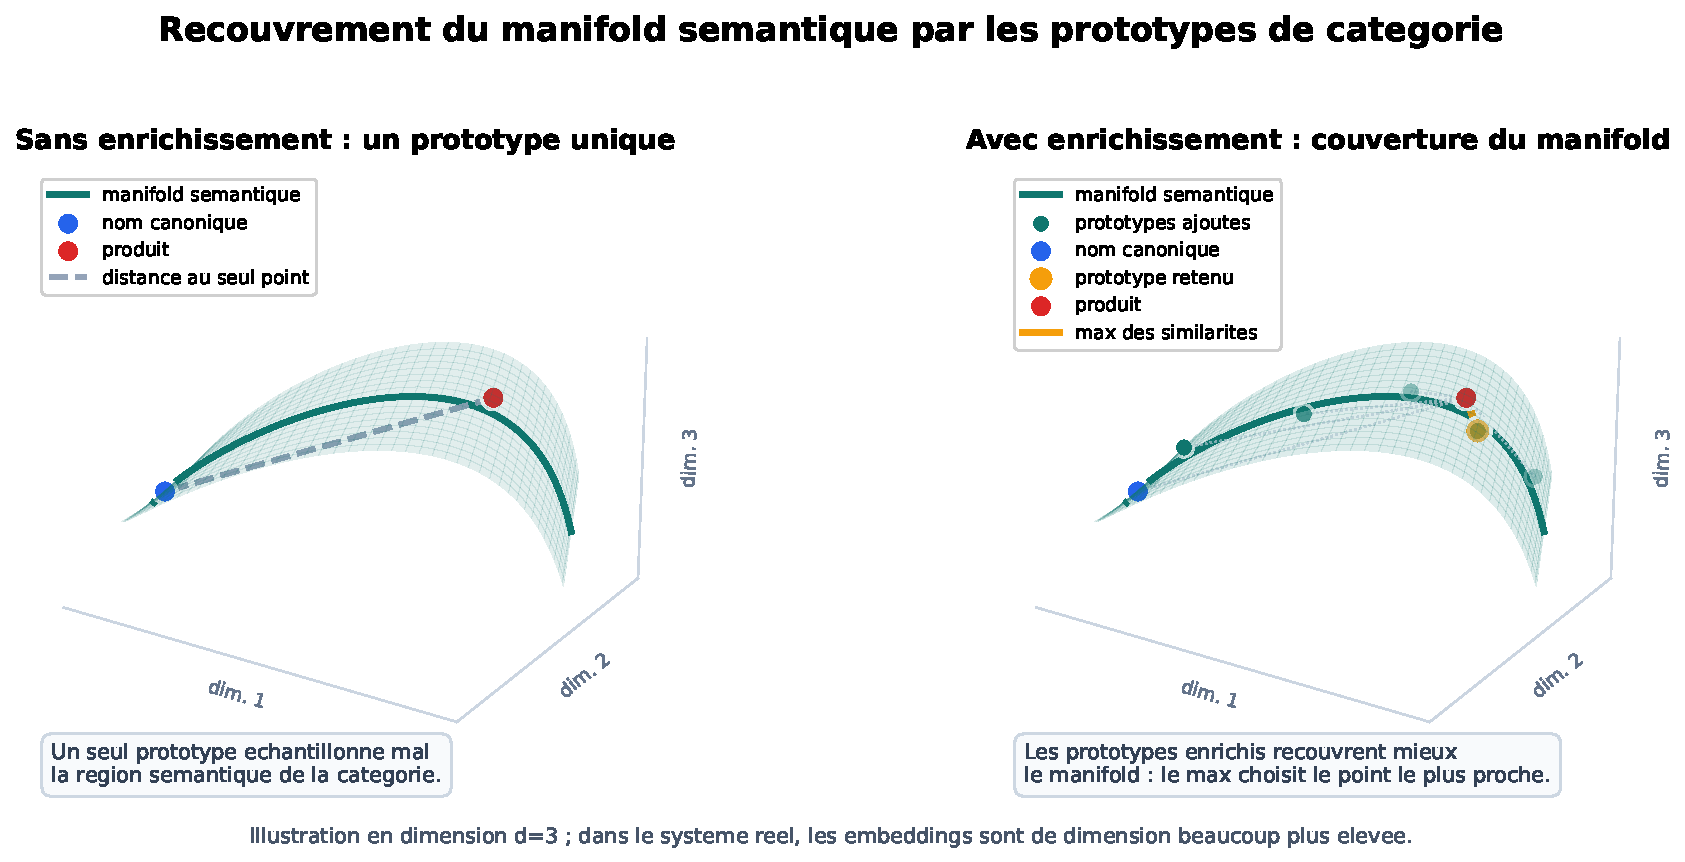
\includegraphics[width=0.96\textwidth]{figures/category_prototype_manifold_coverage.pdf}
    \caption{Recouvrement d'une variété sémantique de catégorie par des prototypes enrichis. La figure est représentée en dimension 3 pour l'intuition, mais elle illustre un espace d'embeddings de dimension beaucoup plus élevée.}
    \label{fig:category-prototype-manifold-coverage-main}
\end{figure}

La figure \ref{fig:category-prototype-manifold-coverage-main} illustre cette idée. Sans enrichissement, la catégorie est représentée par un seul point bleu : le nom de départ. La décision dépend donc d'une distance unique. Avec enrichissement, les prototypes verts couvrent plusieurs zones de la même région sémantique. La catégorie n'est pas transformée en une boule parfaite ; elle est plutôt mieux échantillonnée le long de ses directions sémantiques pertinentes.

Cette intuition devient encore plus importante en grande dimension. Deux catégories proches peuvent avoir des manifolds courbés, partiellement proches ou entrelacés. Dans ce cas, un prototype unique peut tomber dans une zone peu discriminante, alors que plusieurs prototypes permettent de mieux représenter les sous-régions qui séparent réellement les catégories.

\begin{figure}[H]
    \centering
    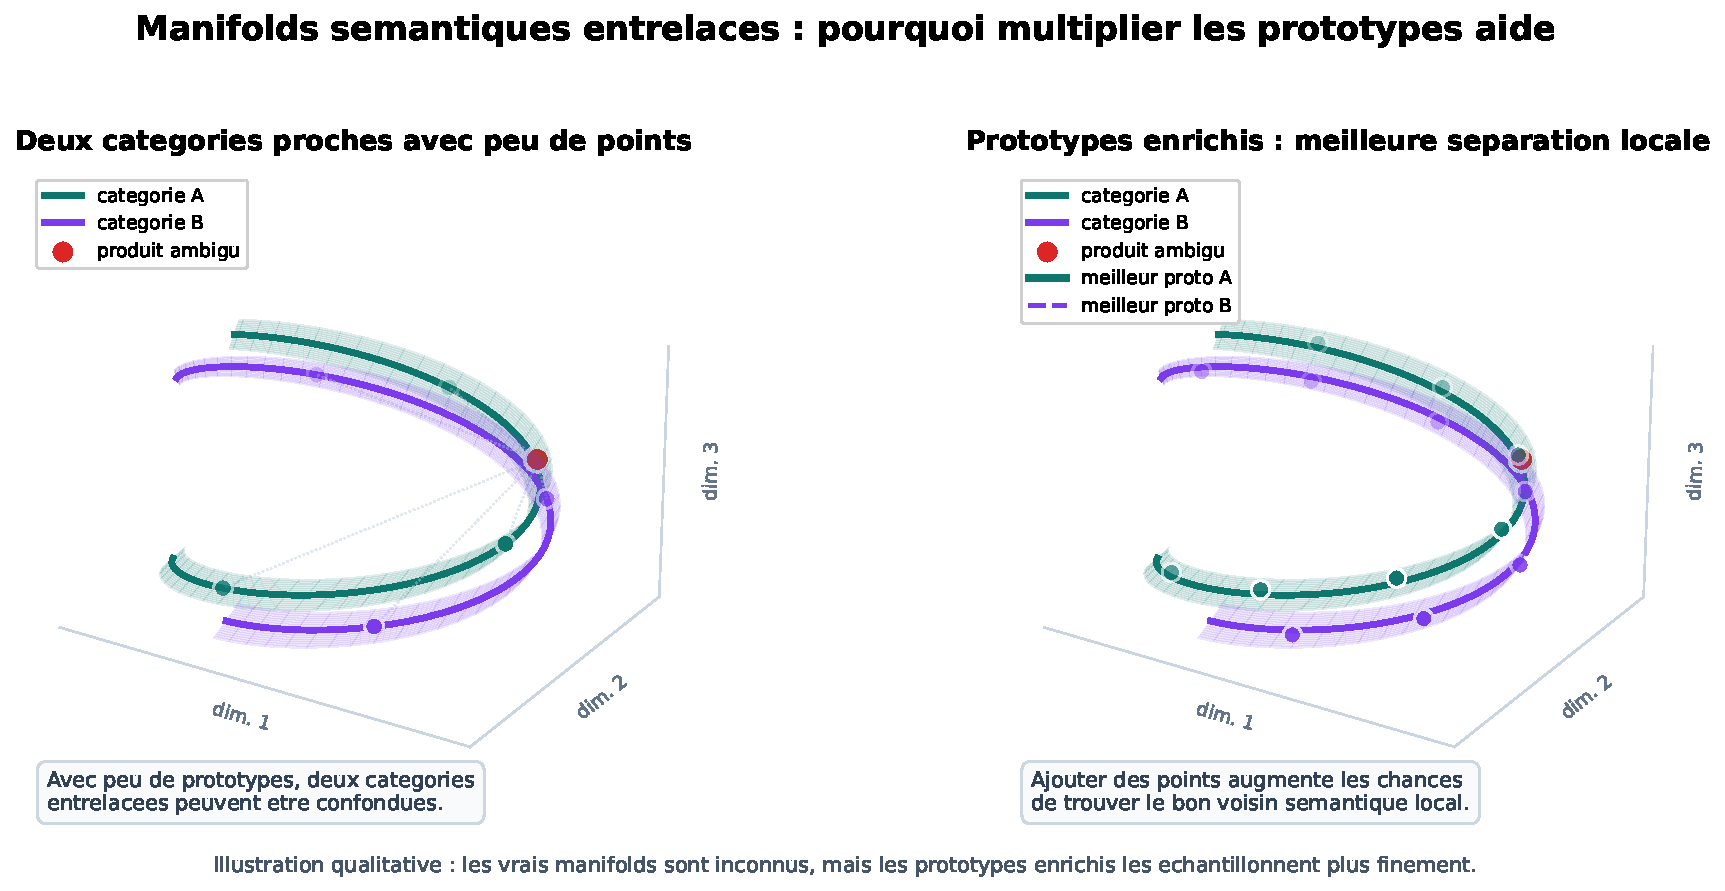
\includegraphics[width=0.70\textwidth]{figures/category_interlaced_manifolds_enrichment.pdf}
    \caption{Illustration de deux manifolds sémantiques proches ou entrelacés dans un espace d'embeddings. L'ajout de prototypes aide à mieux couvrir les régions pertinentes de chaque catégorie.}
    \label{fig:category-interlaced-manifolds-enrichment-main}
\end{figure}

La figure \ref{fig:category-interlaced-manifolds-enrichment-main} montre pourquoi l'enrichissement doit rester contrôlé. Ajouter des prototypes augmente la couverture, mais des prototypes trop génériques peuvent aussi rapprocher artificiellement deux catégories. C'est pourquoi nous utilisons des informations taxonomiques structurées, ainsi que des variantes lexicales générées localement, plutôt qu'une génération libre et non contrainte.
Par exemple, l'ajout systématique des descendants d'une catégorie aurait favorisé l'entrelacement des classes dans l'espace latent, car plusieurs catégories partagent des descendants communs. De même, une génération libre de variantes lexicales peut produire des prototypes trop génériques ou ambigus, qui ne font pas le lien avec les produits spécifiques de la catégorie. En utilisant des variantes lexicales générées localement, nous nous assurons que les prototypes restent proches du vocabulaire métier et qu'ils couvrent des zones pertinentes de la variété sans introduire de bruit sémantique inutile.
L'objectif n'est pas de créer beaucoup de texte, mais de mieux échantillonner les zones de la variété utiles à la recherche sémantique.

La génération des variantes lexicales a d'abord été testée par API, mais cette approche était trop lente et fragile pour plusieurs milliers de catégories. Nous sommes donc passés à une génération locale, qui permet de produire les CSV enrichis sans dépendre d'une limite de débit externe. Cette étape est commune à tout le rapport : le \hyperref[chap:l1-supervised]{Niveau 1 supervisé} et les \hyperref[chap:l2-l7-zero-shot]{pipelines L2--L7} réutilisent ces mêmes prototypes enrichis.

% =======================
% 5. Modélisation supervisée du Niveau 1
% =======================
\chapter{Modélisation supervisée du Niveau 1}
\label{chap:l1-supervised}

Le Niveau 1 est le seul niveau annoté pour tous les produits. Il sert donc de point d'entrée au pipeline complet : une erreur au Niveau 1 contraint ensuite tout le sous-arbre exploré en L2--L7. Nous n'entraînons pas un classifieur, mais un espace métrique où produits et \hyperref[chap:category-enrichment]{prototypes de catégories enrichies} sont comparables par similarité cosinus.

\section{Modèle et objectif d'entraînement}
\label{sec:l1-embedding-choice}
\label{sec:l1-training-objective}

Le modèle retenu est \texttt{BAAI/bge-small-en-v1.5}. Le choix est guidé par le benchmark MTEB, mais surtout par la contrainte industrielle : modèle compact, embeddings de faible dimension et coût d'inférence réduit. Dans la famille des modèles entre environ 10M et 100M paramètres disponibles dans le benchmark, ce modèle offre un compromis solide : 33M paramètres, dimension 384, bonnes performances de classification et de recherche, tout en restant suffisamment petit pour être fine-tuner sur Kaggle.

\begin{table}[H]
    \centering
    \caption{Synthèse du choix de l'encodeur L1}
    \label{tab:l1-mteb-compact-embedders-main}
    \resizebox{\textwidth}{!}{%
    \begin{tabular}{p{4.0cm}p{10.5cm}}
        \toprule
        \textbf{Élément} & \textbf{Synthèse} \\
        \midrule
        Modèle retenu & \texttt{BAAI/bge-small-en-v1.5}, environ 33M paramètres et embeddings de dimension 384. \\
        Justification & Bon compromis entre qualité de recherche, coût mémoire, vitesse d'inférence et faisabilité de le fine-tuning sur Kaggle. \\
        Limite & Le classement MTEB reste un indicateur externe ; la décision finale est validée par les métriques L1 du projet. \\
        \bottomrule
    \end{tabular}
    }
\end{table}

Le tableau détaillé de comparaison MTEB est conservé en annexe, tableau \ref{tab:mteb-compact-embedders}, afin d'éviter une redondance entre le corps principal et les compléments expérimentaux.

\begin{table}[H]
    \centering
    \caption{Configuration finale de le fine-tuning supervisé L1}
    \label{tab:l1-finetuning-hyperparams}
    \resizebox{\textwidth}{!}{%
    \begin{tabular}{ll}
        \toprule
        \textbf{Élément} & \textbf{Valeur} \\
        \midrule
        Modèle initial & \texttt{BAAI/bge-small-en-v1.5}, $\approx$ 33M paramètres, dimension 384 \\
        Training / test & 115\,427 / 12\,826 produits \\
        Loss & Batch Hard Triplet Loss, distance cosinus \\
        Epochs / learning rate / weight decay & 4 / $2 \times 10^{-4}$ / 0{,}01 \\
        Longueur maximale & 256 tokens \\
        Sampling retenu & Tempéré, $\alpha=0{,}5$ \\
        Échantillonneur de lots & $P=8$ catégories, $K=4$ exemples, lot effectif 32 \\
        Optimiseur / scheduler & AdamW / warmup linéaire \\
        \bottomrule
    \end{tabular}
    }
\end{table}

Pour l'inférence, nous réutilisons les prototypes du \hyperref[chap:category-enrichment]{chapitre d'enrichissement}. Pour un produit $x$, la catégorie L1 prédite est celle qui maximise :
\begin{equation}
    S(x,c) = \max_{p \in \mathcal{P}_c} \cos\left(f_\theta(x), f_\theta(p)\right).
\end{equation}
L'entraînement est réalisé sur Kaggle, car nos machines personnelles ne permettaient pas un fine-tuning complet. La longueur de séquence et le batch size ont été limités pour éviter l'explosion de la VRAM.

\begin{figure}[H]
    \centering
    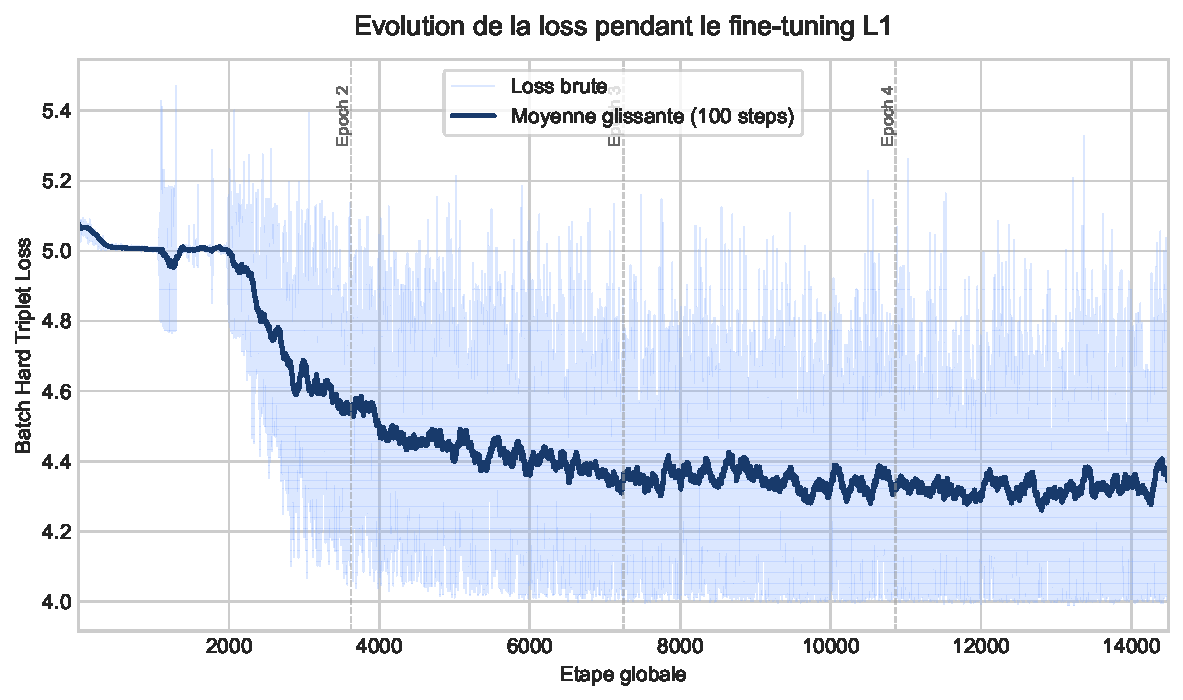
\includegraphics[width=0.82\textwidth]{figures/l1_triplet_loss_alpha05.pdf}
    \caption{Évolution de la perte d'entraînement lors de du fine-tuning supervisé du Niveau 1.}
    \label{fig:l1-triplet-loss-main}
\end{figure}

La figure \ref{fig:l1-triplet-loss-main} montre une baisse régulière de la \textit{Batch Hard Triplet Loss}. Cette baisse ne prouve pas seule la qualité de classification, mais elle confirme que l'espace d'embeddings est effectivement réorganisé : les produits d'une même catégorie sont rapprochés, tandis que les négatifs difficiles sont repoussés. L'évaluation par catégorie est donc indispensable pour vérifier que cette amélioration ne profite pas uniquement aux grandes classes.

\section{Correction du déséquilibre par échantillonnage}
\label{sec:l1-sampling}

Le premier entraînement utilise un échantillonnage naturel : les lots reflètent directement la distribution empirique des catégories. Cette référence atteint une bonne micro-accuracy car elle optimise surtout les catégories fréquentes. Cependant, elle échoue sur plusieurs catégories rares : ces classes apparaissent trop peu souvent dans les lots pour fournir assez de triplets difficiles et informatifs.

\begin{figure}[H]
    \centering
    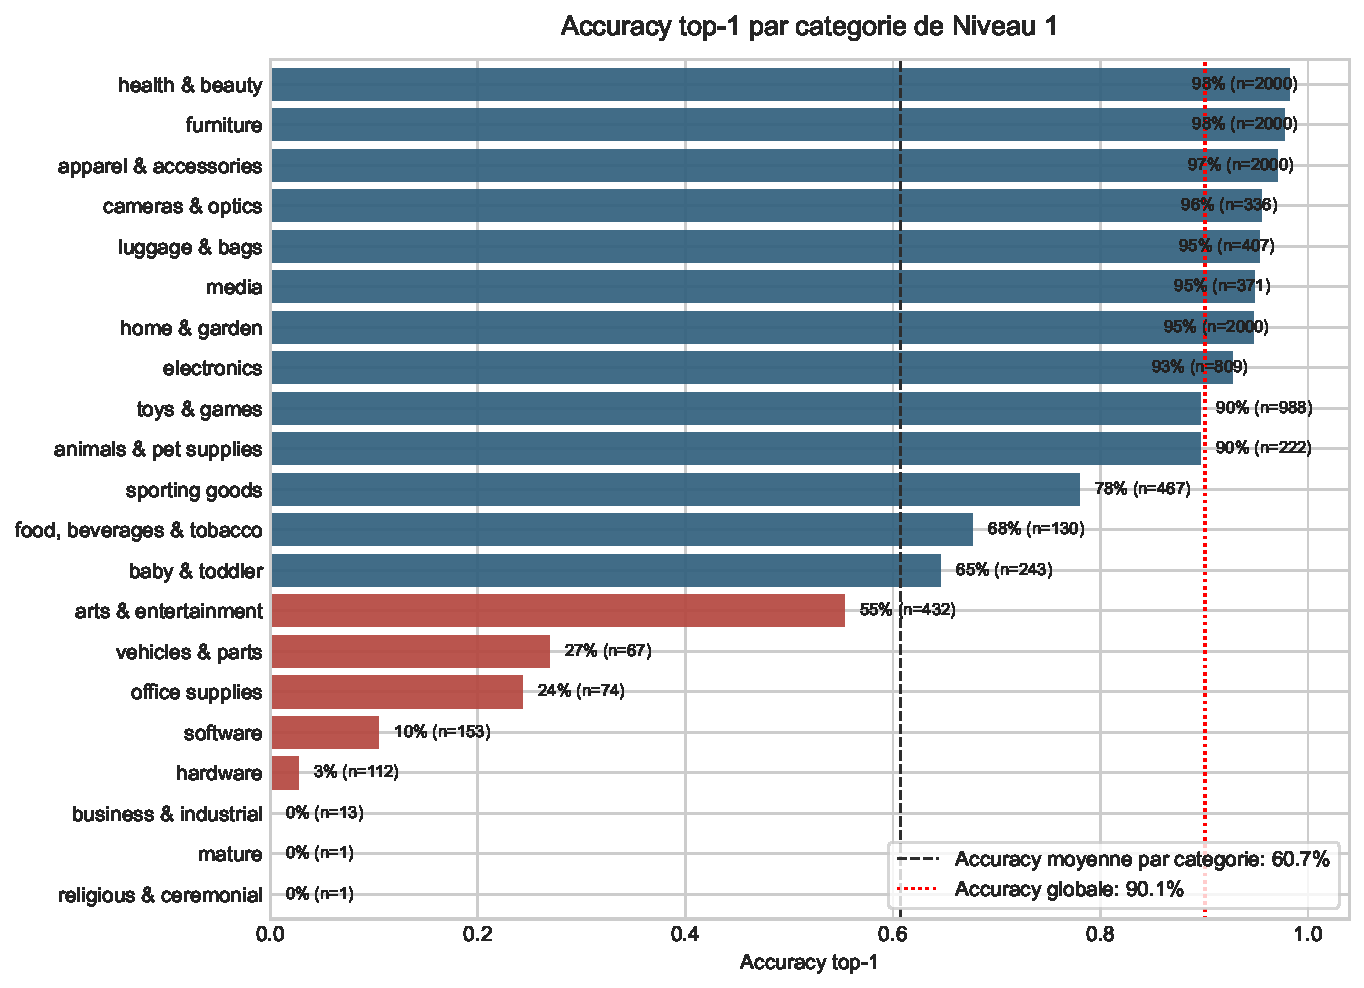
\includegraphics[width=0.48\textwidth]{figures/l1_category_accuracy.pdf}
    \hfill
    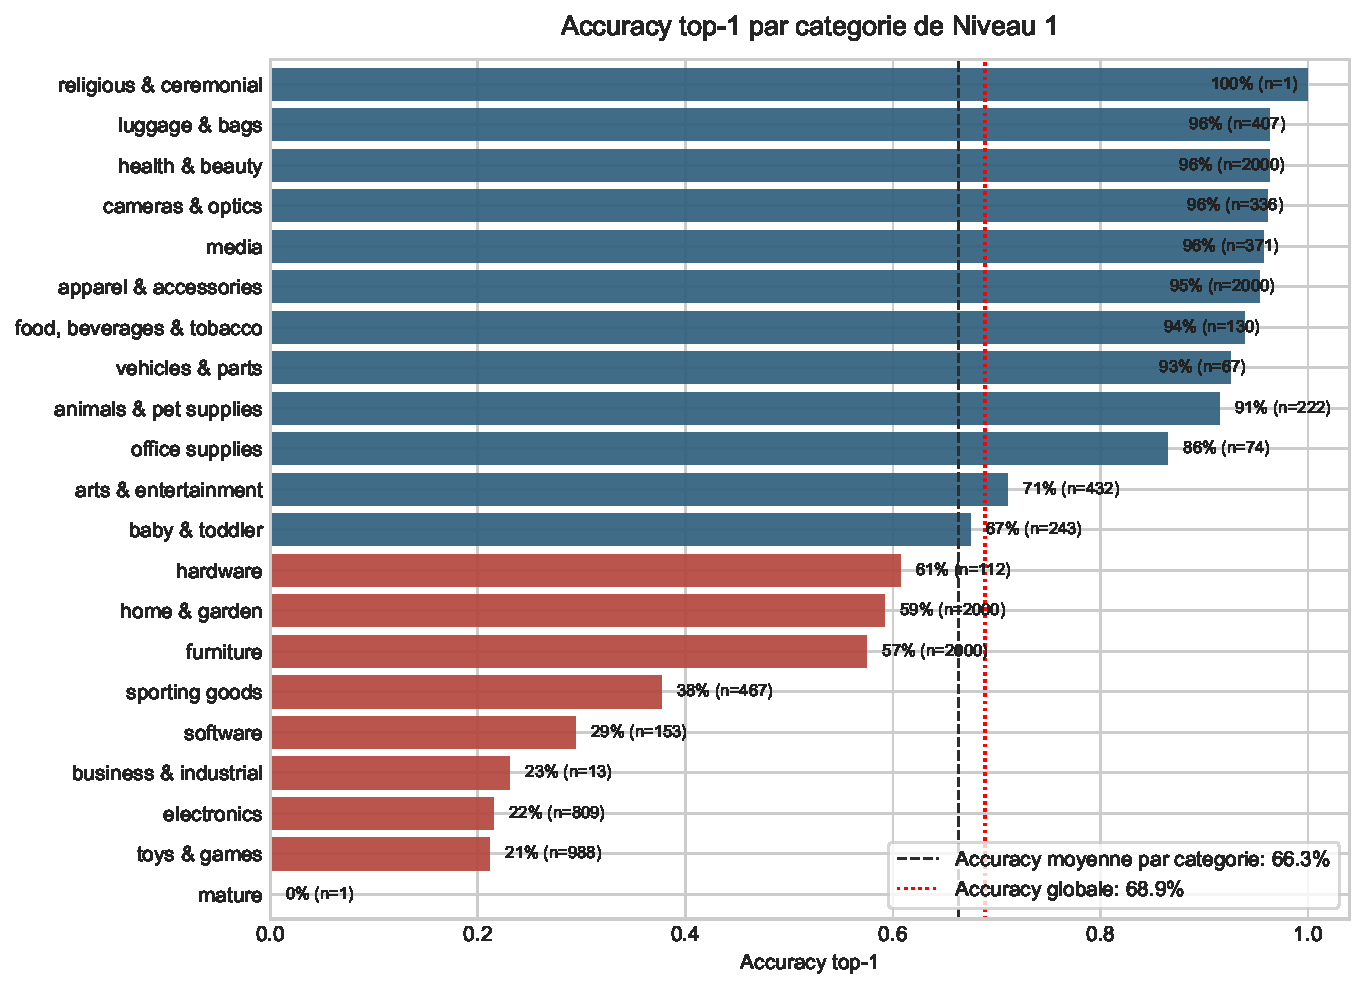
\includegraphics[width=0.48\textwidth]{figures/l1_category_accuracy_balanced_sampling.pdf}
    \caption{accuracy top-1 par catégorie sans échantillonnage équilibré, à gauche, et avec échantillonnage équilibré uniforme, à droite.}
    \label{fig:l1-accuracy-baseline-balanced-main}
\end{figure}

La figure \ref{fig:l1-accuracy-baseline-balanced-main} illustre le problème. Sans échantillonnage équilibré, les grandes catégories dominent l'apprentissage. L'échantillonnage équilibré corrige partiellement ce biais en imposant une présence plus régulière des catégories rares dans les lots. Mais cette correction est trop brutale : les catégories très peu représentées sont sur-échantillonnées, ce qui augmente le risque de surapprentissage et dégrade les catégories qui fonctionnaient déjà bien.

Le compromis retenu est donc un échantillonnage tempéré, où une catégorie $c$ de taille $n_c$ est tirée avec :
\begin{equation}
    \pi_c = \frac{n_c^{\alpha}}{\sum_{c'} n_{c'}^{\alpha}}, \qquad \alpha=0{,}5.
\end{equation}
Le paramètre $\alpha$ contrôle l'intensité de la correction. Avec $\alpha=1$, on retrouve l'échantillonnage naturel proportionnel à la taille des classes. Avec $\alpha=0$, toutes les catégories sont tirées uniformément. La valeur $\alpha=0{,}5$ correspond donc à un compromis : elle augmente fortement la probabilité d'observer les catégories rares, sans ignorer complètement la structure réelle du catalogue.

\begin{table}[H]
    \centering
    \caption{Comparaison globale des stratégies d'échantillonnage L1}
    \label{tab:l1-sampling-results}
    \begin{tabular}{lrr}
        \toprule
        \textbf{Stratégie} & \textbf{Micro-accuracy} & \textbf{Macro-accuracy} \\
        \midrule
        Sans échantillonnage & 90{,}1\,\% & 60{,}7\,\% \\
        Balanced uniforme & 68{,}9\,\% & 66{,}3\,\% \\
        Tempéré $\alpha=0{,}5$ & \textbf{90{,}6\,\%} & \textbf{82{,}8\,\%} \\
        Tempéré $\alpha=0{,}3$ & 89{,}9\,\% & 82{,}4\,\% \\
        Tempéré $\alpha=0{,}8$ & \textbf{92{,}4\,\%} & 80{,}5\,\% \\
        \bottomrule
    \end{tabular}
\end{table}

Le modèle $\alpha=0{,}5$ est retenu car il maximise la macro-accuracy tout en gardant une micro-accuracy élevée. Le modèle $\alpha=0{,}8$ obtient la meilleure micro-accuracy, mais il corrige moins fortement les catégories rares. À l'inverse, l'échantillonnage équilibré uniforme améliore certaines petites classes mais sacrifie trop la performance globale. Le choix final privilégie donc le compromis industriel : conserver une très bonne performance sur le catalogue tout en réduisant le risque d'ignorer systématiquement les branches rares.

Le détail par catégorie est donné en annexe dans la figure \ref{fig:l1-category-accuracy-sampling-comparison}. Cette figure confirme que le gain de l'échantillonnage tempéré est surtout visible sur les catégories minoritaires. Les stratégies trop équilibrées peuvent faire chuter des catégories fréquentes, tandis que les stratégies trop proches de l'échantillonnage naturel conservent les défauts initiaux. L'échantillonnage tempéré agit donc comme une régularisation de la distribution des lots.

\section{Visualisation de l'espace appris}
\label{sec:l1-umap-main}

Pour vérifier qualitativement que le fine-tuning modifie bien la géométrie de l'espace latent, nous projetons les embeddings produits en deux dimensions avec UMAP. L'objectif n'est pas de mesurer des distances exactes en 2D, mais d'inspecter les voisinages locaux et la séparation globale des catégories.

\begin{figure}[H]
    \centering
    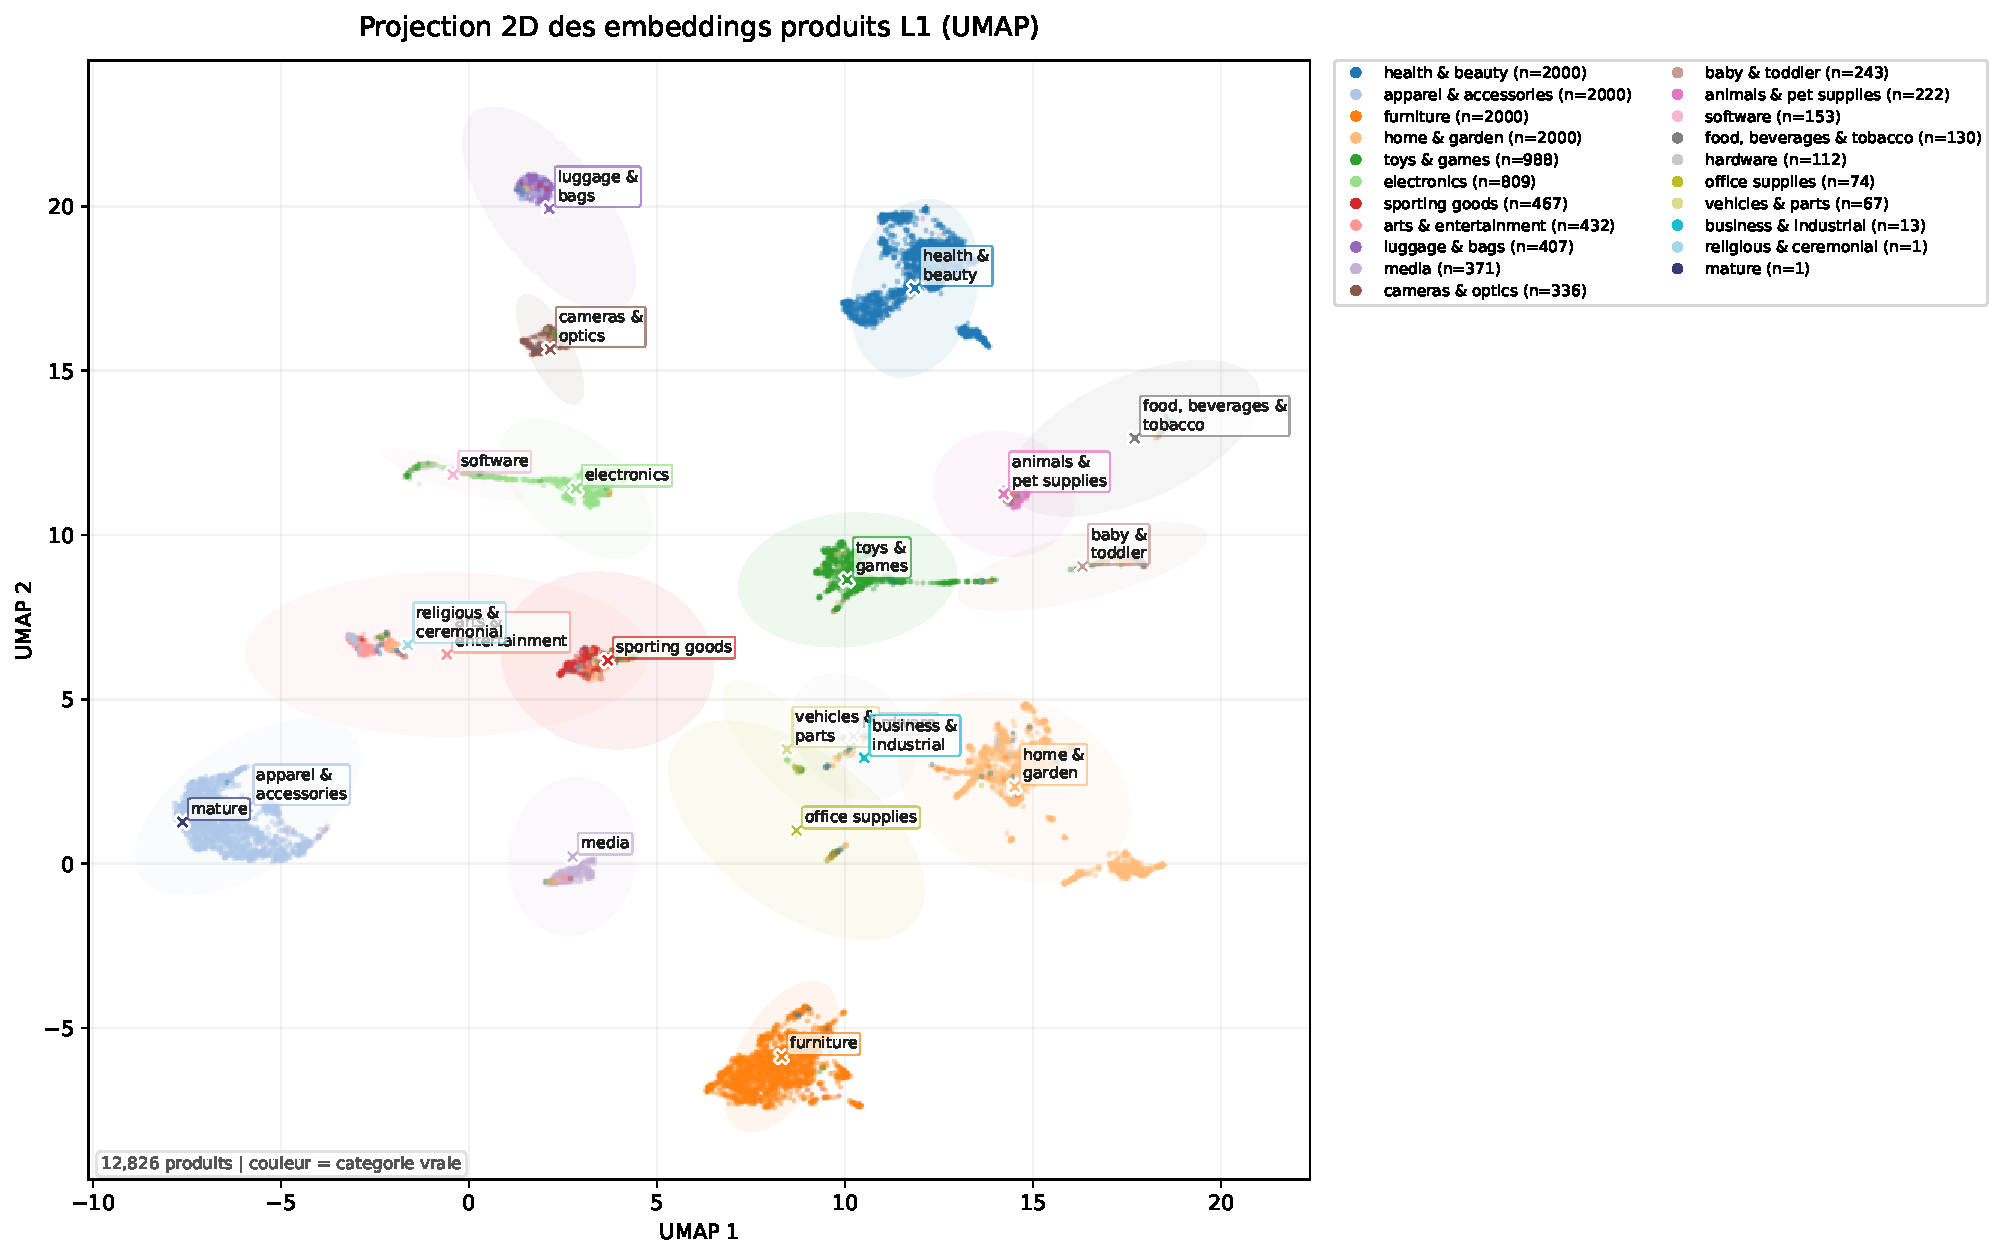
\includegraphics[width=1.10\textwidth]{figures/l1_embedding_projection_umap.pdf}
    \caption{Projection UMAP des embeddings produits après fine-tuning supervisé du Niveau 1.}
    \label{fig:l1-embedding-umap-main}
\end{figure}

La figure \ref{fig:l1-embedding-umap-main} montre que les catégories nombreuses forment des régions bien séparées dans l'espace projeté. Cela confirme que le fine-tuning ne se contente pas d'améliorer une métrique numérique : il structure réellement l'espace d'embeddings autour des grandes familles taxonomiques. Les catégories rares restent moins nettes, ce qui est cohérent avec le manque d'exemples et avec les écarts de macro-métriques observés.

\section{Métriques finales de classification}
\label{sec:l1-final-metrics}

\begin{table}[H]
    \centering
    \caption{Métriques finales de classification du modèle Niveau 1 retenu}
    \label{tab:l1-final-classification-metrics}
    \begin{tabular}{lr}
        \toprule
        \textbf{Métrique} & \textbf{Valeur} \\
        \midrule
        accuracy top-1 / micro-$F_1$ & 90{,}6\,\% \\
        accuracy top-3 & 95{,}5\,\% \\
        accuracy top-5 & 97{,}1\,\% \\
        Macro-précision & 74{,}8\,\% \\
        Macro-recall / accuracy équilibrée & 82{,}8\,\% \\
        Macro-$F_1$ & 77{,}7\,\% \\
        $F_1$ pondéré & 90{,}9\,\% \\
        \bottomrule
    \end{tabular}
\end{table}

Les définitions et formules des métriques du tableau \ref{tab:l1-final-classification-metrics} sont détaillées en \hyperref[sec:l1-classification-metrics-annex]{annexe}.\\

Le modèle L1 retenu atteint 90{,}6\,\% d'accuracy top-1 et 97{,}1\,\% d'accuracy top-5, avec un $F_1$ pondéré de 90{,}9\,\%. La matrice de confusion détaillée est déplacée en annexe, figure \ref{fig:l1-confusion-matrix-normalized}, pour garder le corps principal centré sur la synthèse.

Ces résultats indiquent que le Niveau 1 est suffisamment robuste pour servir de point d'entrée au pipeline L2--L7. Le top-5 élevé montre que, même lorsque le top-1 est incorrect, la bonne catégorie reste souvent proche dans l'espace sémantique, ce qui justifie l'usage de méthodes conservant plusieurs hypothèses, comme le beam search.

Les performances L1 ne garantissent pas la qualité des niveaux profonds. Une erreur au Niveau 1 contraint tout le sous-arbre exploré ensuite, et l'absence de labels L2--L7 empêche de transformer cette robustesse locale en mesure d'accuracy globale.

% =======================
% 6. Recherche zéro-shot pour L2--L7
% =======================
\chapter{Recherche zéro-shot pour L2--L7}
\label{chap:l2-l7-zero-shot}

Les niveaux 2 à 7 ne disposent pas de labels supervisés fiables. Nous ne pouvons donc pas annoncer une accuracy classique ; nous comparons plutôt des hypothèses taxonomiques produites par plusieurs pipelines. Tous partent du même Niveau 1 fine-tuner, puis utilisent les \hyperref[chap:category-enrichment]{catégories enrichies} pour descendre ou retrouver un chemin dans la taxonomie.

\section{Embeddings partagés et choix de l'encodeur}
\label{sec:l2-l7-embedder-comparison}

Deux encodeurs compacts sont testés : \texttt{Qwen3} et \texttt{Jasper}. Ils encodent les mêmes 128\,253 produits, 32\,884 prototypes enrichis et 5\,406 chemins taxonomiques. Les noms complets des modèles sont reportés dans le tableau \ref{tab:l2-l7-embedding-generation-comparison}.

\begin{table}[H]
    \centering
    \caption{Coût de génération des embeddings partagés L2--L7}
    \label{tab:l2-l7-embedding-generation-comparison}
    \resizebox{\textwidth}{!}{%
    \begin{tabular}{lrrrrrr}
        \toprule
        \textbf{Encodeur} & \textbf{Dim.} & \textbf{Temps export} & \textbf{Textes/s} & \textbf{Taille matrices} & \textbf{Mémoire GPU pic} & \textbf{Coût token-dimension} \\
        \midrule
        \texttt{Qwen3-Embedding-0.6B} & \textbf{1024} & 163{,}2 min & 17{,}0 & \textbf{650{,}6 MB} & 7659{,}0 MB & \textbf{15\,175{,}3 M} \\
        \texttt{Jasper-Token-Compression-600M} & 2048 & \textbf{121{,}6 min} & \textbf{22{,}8} & 1301{,}1 MB & \textbf{2774{,}9 MB} & 30\,350{,}6 M \\
        \bottomrule
    \end{tabular}
    }
\end{table}

Jasper encode plus vite dans notre run Kaggle, mais ses embeddings de dimension 2048 doublent la taille mémoire et le coût vectoriel par rapport à Qwen3. Ce point est visible dans le tableau \ref{tab:l2-l7-embedding-generation-comparison}. Pour un catalogue très volumineux, le coût le plus important n'est pas seulement le temps initial d'encodage : c'est aussi la taille des matrices à stocker, charger, transférer et comparer à chaque étape de recherche.

\paragraph{Contexte matériel du benchmark.}
Les mesures de cette section ont été obtenues dans l'environnement Kaggle utilisé pour le projet, avec une exécution sur deux GPU T4 et un batch size de 64 pour les exports d'embeddings. Les matrices chargées correspondent à 128\,253 produits, 32\,884 prototypes enrichis et 5\,406 chemins taxonomiques, avec 650{,}6 MB pour Qwen3 et 1\,301{,}1 MB pour Jasper.

\section{Méthodologie d'évaluation non supervisée}
\label{sec:l2-l7-unsupervised-metrics}

Nous utilisons trois familles de métriques. La première mesure le coût d'inférence. Pour un pipeline $m$ appliqué à $N$ produits, nous mesurons le temps total $T_m$, le temps moyen
\begin{equation}
    \bar{t}_m=\frac{T_m}{N},
\end{equation}
le débit $N/T_m$, la mémoire chargée et un coût vectoriel approximatif. Si le pipeline calcule $q_m$ produits scalaires entre embeddings de dimension $d$, alors le nombre d'opérations scalaires est approximé par $q_m d$. Cette métrique ne remplace pas une mesure réelle de latence, mais elle permet de comparer deux encodeurs d'embeddings de dimensions différentes, notamment Qwen3 en dimension 1024 et Jasper en dimension 2048.

La deuxième famille mesure la confiance interne. Pour les pipelines qui produisent plusieurs candidats, la marge top-1/top-2 est
\begin{equation}
    \Delta(x)=S_1(x)-S_2(x),
\end{equation}
où $S_1$ et $S_2$ sont les scores des deux meilleurs chemins. Une marge faible signifie que la décision est instable : deux chemins taxonomiques restent presque aussi plausibles. Nous mesurons aussi la profondeur moyenne prédite, le nombre de chemins distincts, la part du chemin le plus fréquent et l'entropie de la distribution des chemins :
\begin{equation}
    H=-\sum_h p(h)\log p(h).
\end{equation}
Une méthode qui prédit très profond avec une marge faible est plus risquée qu'une méthode qui s'arrête plus tôt mais avec une décision plus nette.

La troisième famille compare les pipelines entre eux. Le Niveau 1 est fixé par le même modèle fine-tuner pour toutes les méthodes ; il ne constitue donc pas une métrique de comparaison pertinente. La comparaison porte sur les niveaux réellement non supervisés : accord exact sur le chemin complet, accord niveau par niveau L2--L7 et V de Cramér pour mesurer l'association entre labels discrets. Pour deux pipelines $A$ et $B$, l'accord au niveau $\ell$ est
\begin{equation}
    \operatorname{Acc}_{\ell}(A,B)
    =
    \frac{1}{n_\ell}
    \sum_{i=1}^{n_\ell}
    \mathbf{1}
    \left[
    \hat{y}^{A}_{i,\ell}
    =
    \hat{y}^{B}_{i,\ell}
    \right].
\end{equation}
Les définitions détaillées sont données en \hyperref[sec:l2-l7-metrics-annex]{annexe}, avec le V de Cramér en \hyperref[sec:cramers-v-annex]{annexe dédiée}.

Enfin, nous ajoutons un audit NLP externe. Pour chaque produit, les chemins proposés par les pipelines sont scorés par un bi-encodeur et par un cross-encodeur. Ces scores ne remplacent pas une vérité terrain ; ils servent à comparer les propositions concurrentes d'un même produit.

\section{Pipeline 1 : décodage hiérarchique local}
\label{sec:l2-l7-pipeline1-local-decoding-main}

Le premier pipeline suit explicitement la structure de la taxonomie. Après la prédiction du Niveau 1 par le modèle fine-tuner, on se place dans le sous-arbre correspondant et on compare le produit aux enfants du nœud courant. Pour un produit $x$, un nœud parent $u$ et un enfant candidat $c\in\operatorname{Child}(u)$, le score local est
\begin{equation}
    s(x,c)
    =
    \max_{p\in\mathcal{P}_c}
    \cos(g(x),g(p)),
\end{equation}
où $g$ est l'encodeur L2--L7 et $\mathcal{P}_c$ l'ensemble des prototypes enrichis de la catégorie $c$.

La variante greedy choisit l'enfant de score maximal à chaque niveau :
\begin{equation}
    \hat{c}_{\ell}
    =
    \arg\max_{c\in\operatorname{Child}(\hat{c}_{\ell-1})}
    s(x,c).
\end{equation}
Elle est très rapide car elle ne conserve qu'un seul chemin. Sa limite est la propagation d'erreur : une mauvaise décision au Niveau 2 empêche ensuite d'explorer la bonne branche aux niveaux inférieurs.

Le beam search corrige partiellement ce défaut en conservant plusieurs chemins partiels. Un chemin $h=(\hat{c}_1,\ldots,\hat{c}_\ell)$ reçoit un score cumulé :
\begin{equation}
    S(h\mid x)=\sum_{t=2}^{\ell}s(x,\hat{c}_t).
\end{equation}
À chaque profondeur, seuls les $B$ meilleurs chemins sont conservés. Cette méthode est plus coûteuse que le greedy, mais elle évite de prendre une décision irréversible trop tôt. Enfin, la variante beam + reranker conserve les meilleurs chemins du beam puis les reclasse avec un modèle de ranking externe. Le détail algorithmique complet du beam search et du reranking est donné en \hyperref[sec:beam-reranker-annex]{annexe}.

\section{Pipeline 2 : clustering hiérarchique contraint par la taxonomie}
\label{sec:l2-l7-pipeline2-clustering-main}

Le deuxième pipeline exploite une hypothèse différente : les produits d'une même branche taxonomique doivent former des groupes dans l'espace d'embeddings. Pour prédire le Niveau 2 dans une branche L1 donnée, on récupère les produits rattachés à cette branche par le modèle L1, puis on lit dans la taxonomie le nombre d'enfants $K$ du nœud. On entraîne alors un clustering avec $K$ clusters dans les embeddings produits :
\begin{equation}
    \min_{\mu_1,\ldots,\mu_K}
    \sum_{i=1}^{n}
    \min_{k\in\{1,\ldots,K\}}
    \|z_i-\mu_k\|_2^2.
\end{equation}
Chaque centroïde $\mu_k$ doit ensuite être associé à une catégorie enfant. Nous construisons une matrice de coût fondée sur la similarité entre centroïdes et prototypes enrichis :
\begin{equation}
    C_{k,c}
    =
    -\max_{p\in\mathcal{P}_c}\cos(\mu_k,g(p)).
\end{equation}
L'affectation cluster--catégorie est résolue globalement, par exemple avec une affectation hongroise lorsque le problème est équilibré. Le même principe est ensuite répété niveau par niveau. Cette méthode peut révéler une structure collective du catalogue, mais elle suppose que les catégories taxonomiques correspondent bien à des clusters géométriques observables. Si une catégorie enfant n'est pas présente dans les produits ou si deux enfants sont lexicalement très proches, le clustering peut créer des groupes artificiels.

\section{Pipeline 3 : recherche de chemins globaux}
\label{sec:l2-l7-pipeline3-global-path-main}

Le troisième pipeline évite la descente locale. Chaque chemin complet de la taxonomie est transformé en texte, par exemple en concaténant les noms des catégories du Niveau 2 jusqu'au nœud final, puis encodé une seule fois. Pour un produit $x$, la prédiction est obtenue par plus proche voisin parmi les chemins compatibles avec le Niveau 1 prédit :
\begin{equation}
    \hat{h}
    =
    \arg\max_{h\in\mathcal{H}(\hat{c}_1)}
    \cos(g(x),g(h)).
\end{equation}
Cette méthode compare directement le produit à une hypothèse taxonomique globale. Elle peut donc éviter certaines erreurs locales du greedy, car elle ne choisit pas séparément chaque niveau. En revanche, plusieurs chemins complets peuvent être très proches lexicalement, ce qui produit souvent des marges top-1/top-2 faibles. La recherche de chemins globaux est donc utile comme référence de diversité et comme méthode de désaccord, mais il est moins directement interprétable qu'une descente hiérarchique locale.


\section{Pipelines comparés}
\label{sec:l2-l7-pipeline-local-decoding}
\label{sec:l2-l7-pipeline-clustering}
\label{sec:l2-l7-pipeline-global-path}

\begin{table}[H]
    \centering
    \caption{Résumé des pipelines zéro-shot L2--L7}
    \label{tab:l2-l7-pipeline-summary}
    \resizebox{\textwidth}{!}{%
    \begin{tabular}{p{3.1cm}p{5.4cm}p{4.0cm}p{4.0cm}}
        \toprule
        \textbf{Pipeline} & \textbf{Principe} & \textbf{Avantage} & \textbf{Limite} \\
        \midrule
        Greedy & Descente locale : à chaque niveau, choisir l'enfant le plus proche du produit. & Très rapide, faible mémoire, simple à industrialiser. & Une erreur haute dans l'arbre est irréversible. \\
        Beam search & Conserver plusieurs chemins candidats à chaque niveau. & Réduit le risque d'une décision locale trop précoce. & Coût supérieur au greedy et marges souvent faibles. \\
        Beam + reranker & Reranker les meilleurs chemins du beam avec un modèle externe. & Meilleure qualité NLP brute. & Trop coûteux pour tous les produits. \\
        Clustering & Grouper les produits par branche L1, puis associer les clusters aux enfants taxonomiques. & Capture une structure collective du catalogue. & Peut créer des groupes artificiels si certaines catégories sont absentes. \\
        Recherche globale & Comparer directement le produit aux embeddings des chemins complets. & Très diversifié et évite la descente locale. & Marges faibles et risque de chemins concurrents proches. \\
        \bottomrule
    \end{tabular}
    }
\end{table}



\section{Résultats synthétiques}
\label{sec:l2-l7-pipeline-agreement}

Le tableau suivant rassemble les résultats essentiels. Il ne mesure pas une accuracy, mais le compromis entre coût, profondeur, diversité et concentration des prédictions.

\begin{table}[H]
    \centering
    \caption{Synthèse des résultats L2--L7 par embedder et par pipeline}
    \label{tab:l2-l7-embedder-pipeline-results}
    \scriptsize
    \resizebox{\textwidth}{!}{%
    \begin{tabular}{llrrrrrr}
        \toprule
        \textbf{Embedder} & \textbf{Pipeline} & \textbf{ms/prod.} & \textbf{M ops/prod.} & \textbf{Mémoire} & \textbf{Prof. moy.} & \textbf{Chemins} & \textbf{Top chemin} \\
        \midrule
        Qwen3 & \textbf{Greedy} & \textbf{1{,}14} & \textbf{0{,}39} & \textbf{629 MB} & 3{,}08 & 2\,186 & 2{,}1\,\% \\
        Qwen3 & Beam & 2{,}71 & 0{,}62 & 629 MB & 3{,}22 & 2\,461 & 1{,}8\,\% \\
        Qwen3 & Beam + reranker & 16{,}17 & 0{,}62 + rerank & 629 MB & 3{,}21 & 2\,679 & 1{,}5\,\% \\
        Qwen3 & Clustering & 0{,}71 & 0{,}42 & 629 MB & 3{,}01 & 3\,121 & 2{,}6\,\% \\
        Qwen3 & Recherche globale & 1{,}67 & 0{,}51 & 651 MB & \textbf{3{,}37} & \textbf{3\,337} & 1{,}8\,\% \\
        Jasper & Greedy & 1{,}12 & 0{,}77 & 1259 MB & 3{,}01 & 2\,274 & 8{,}5\,\% \\
        Jasper & Beam & 2{,}84 & 1{,}21 & 1259 MB & 3{,}10 & 2\,580 & 8{,}5\,\% \\
        Jasper & Beam + reranker & 15{,}82 & 1{,}21 + rerank & 1259 MB & 3{,}13 & 2\,831 & 2{,}8\,\% \\
        Jasper & Clustering & 1{,}00 & 0{,}87 & 1259 MB & 2{,}98 & 3\,098 & 2{,}8\,\% \\
        Jasper & Recherche globale & 1{,}67 & 1{,}01 & 1301 MB & 3{,}16 & 3\,013 & 8{,}4\,\% \\
        \bottomrule
    \end{tabular}
    }
\end{table}

La pipeline greedy est le meilleur compromis de coût d'inférence : environ 1{,}14 ms par produit avec Qwen3. Le passage de greedy à beam augmente modérément le coût, tandis que l'ajout d'un reranker change d'ordre de grandeur et atteint environ 16 ms par produit.

La recherche globale produit les chemins les plus diversifiés avec Qwen3, mais ses marges top-1/top-2 restent faibles. Le beam search améliore l'exploration par rapport au greedy, sans justifier à lui seul un reranking systématique sur tout le catalogue.

Ces résultats ne sont pas des mesures d'accuracy L2--L7. Ils décrivent un compromis entre coût, profondeur, diversité et stabilité interne. Les figures et matrices détaillées de divergence sont données en \hyperref[sec:l2-l7-family3-matrices-annex]{annexe}.

\begin{table}[H]
    \centering
    \caption{Synthèse globale des accords entre pipelines}
    \label{tab:l2-l7-family3-global-summary}
    \resizebox{\textwidth}{!}{%
    \begin{tabular}{lrrrrrrrr}
        \toprule
        \textbf{Embedder} & \textbf{Produits} & \textbf{Même chemin} & \textbf{Chemins/prod.} & \textbf{Accord moyen} & \textbf{$V$ moyen} & \textbf{Même L2} & \textbf{Même L3} & \textbf{Dernier niveau commun} \\
        \midrule
        Qwen3 & 128\,253 & 1{,}3\,\% & 3{,}42 & 23{,}6\,\% & 0{,}426 & 15{,}0\,\% & 13{,}1\,\% & 2{,}49 \\
        Jasper & 128\,253 & 1{,}9\,\% & 3{,}24 & 27{,}2\,\% & 0{,}446 & 13{,}6\,\% & 19{,}8\,\% & 2{,}46 \\
        \bottomrule
    \end{tabular}
    }
\end{table}

\begin{figure}[H]
    \centering
    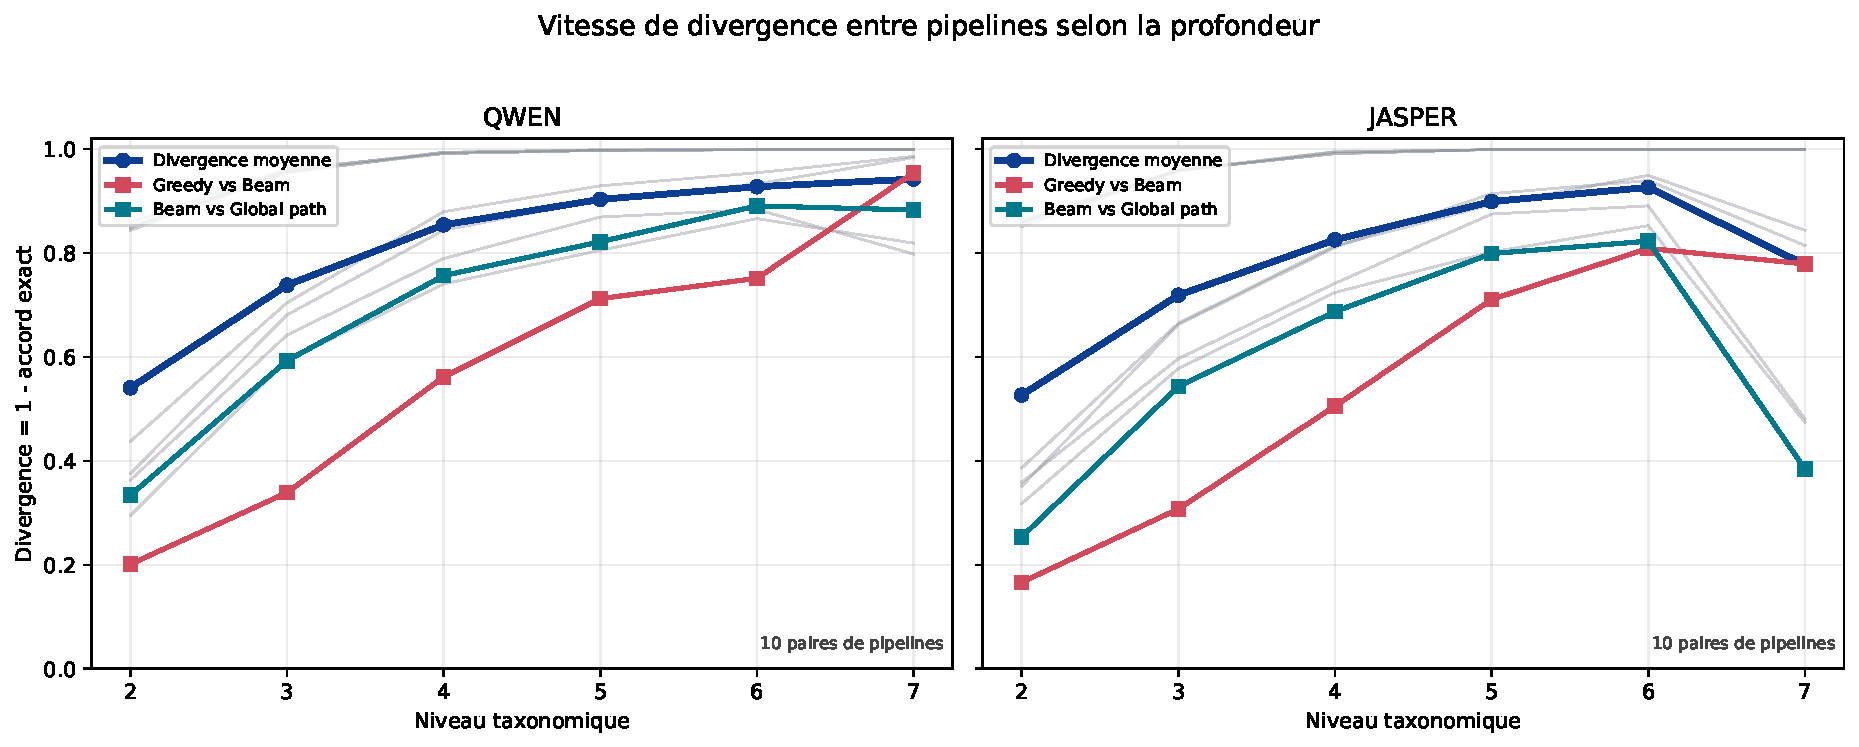
\includegraphics[width=0.92\textwidth]{figures/l2_l7_family3_annex/family3_divergence_by_depth.pdf}
    \caption{Vitesse de divergence entre pipelines selon la profondeur taxonomique.}
    \label{fig:l2-l7-family3-divergence-depth-main}
\end{figure}

Les pipelines convergent rarement tous vers le même chemin complet, et la figure \ref{fig:l2-l7-family3-divergence-depth-main} montre que le désaccord augmente rapidement avec la profondeur.

Les méthodes peuvent encore partager une décision générale en L2, puis diverger en L3 ou L4 lorsque les distinctions deviennent plus fines. Greedy et beam restent les méthodes les plus proches, tandis que le clustering est volontairement plus éloigné car il optimise une partition collective plutôt qu'une décision produit par produit.

Cette divergence est attendue en l'absence de labels L2--L7 : chaque pipeline explore une hypothèse différente, sans qu'il soit possible de désigner automatiquement la bonne prédiction.

\begin{figure}[H]
    \centering
    
\includegraphics[width=0.48\textwidth]{figures/l2_l7_family3_qwen/family3_exact_path_agreement_heatmap.pdf}
    \hfill
    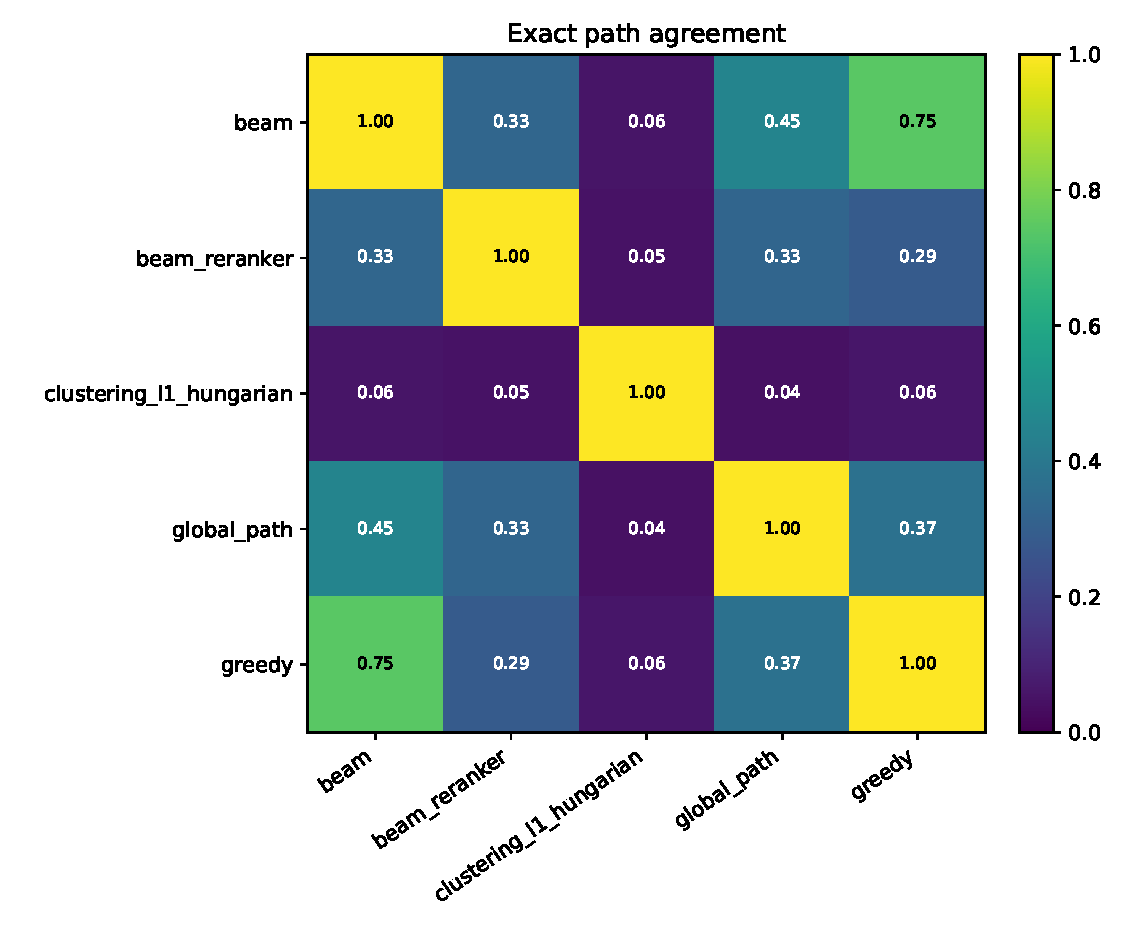
\includegraphics[width=0.48\textwidth]{figures/l2_l7_family3_jasper/family3_exact_path_agreement_heatmap.pdf}
    \caption{Matrices d'accord exact sur le chemin complet pour Qwen3, à gauche, et Jasper, à droite.}
    \label{fig:l2-l7-exact-path-agreement-main}
\end{figure}

La figure \ref{fig:l2-l7-exact-path-agreement-main} confirme que les accords forts sont concentrés sur les variantes proches du même pipeline, notamment greedy et beam.
Les désaccords servent à identifier les produits pour lesquels une validation humaine, un reranker ou une stratégie hybride serait utile.
Ils ne doivent pas être lus comme des erreurs certaines, car aucune vérité terrain L2--L7 n'est disponible.

\begin{table}[H]
    \centering
    \caption{Audit NLP complet : score moyen, win rate et rang moyen}
    \label{tab:l2-l7-full-biencoder-audit}
    \scriptsize
    \resizebox{\textwidth}{!}{%
    \begin{tabular}{llrrrrrr}
        \toprule
        \textbf{Scorer} & \textbf{Pipeline} & \textbf{Score Qwen} & \textbf{Win Qwen} & \textbf{Rang Qwen} & \textbf{Score Jasper} & \textbf{Win Jasper} & \textbf{Rang Jasper} \\
        \midrule
        Bi-encodeur & Greedy & 0{,}260 & \textbf{29{,}5\,\%} & \textbf{2{,}50} & 0{,}262 & \textbf{31{,}9\,\%} & \textbf{2{,}39} \\
        Bi-encodeur & Beam & 0{,}273 & 10{,}4\,\% & 2{,}91 & 0{,}275 & 9{,}8\,\% & 2{,}86 \\
        Bi-encodeur & Beam + reranker & 0{,}272 & 18{,}4\,\% & 3{,}02 & 0{,}270 & 17{,}2\,\% & 3{,}13 \\
        Bi-encodeur & Clustering & 0{,}227 & 21{,}6\,\% & 3{,}63 & 0{,}224 & 21{,}8\,\% & 3{,}64 \\
        Bi-encodeur & Recherche globale & \textbf{0{,}288} & 20{,}1\,\% & 2{,}94 & \textbf{0{,}293} & 19{,}3\,\% & 2{,}97 \\
        Cross-encodeur & Greedy & -4{,}724 & 17{,}0\,\% & 2{,}92 & -4{,}654 & 18{,}3\,\% & 2{,}81 \\
        Cross-encodeur & Beam & -4{,}618 & 7{,}9\,\% & 3{,}31 & -4{,}561 & 7{,}8\,\% & 3{,}25 \\
        Cross-encodeur & Beam + reranker & \textbf{-4{,}248} & \textbf{37{,}5\,\%} & \textbf{2{,}15} & \textbf{-4{,}221} & \textbf{39{,}4\,\%} & \textbf{2{,}14} \\
        Cross-encodeur & Clustering & -4{,}882 & 21{,}7\,\% & 3{,}53 & -4{,}885 & 20{,}2\,\% & 3{,}63 \\
        Cross-encodeur & Recherche globale & -4{,}400 & 15{,}9\,\% & 3{,}09 & -4{,}382 & 14{,}3\,\% & 3{,}17 \\
        \bottomrule
    \end{tabular}
    }
\end{table}

L'audit NLP clarifie le compromis. Le bi-encodeur favorise la recherche de chemins globaux en score moyen, car ce pipeline optimise directement une similarité produit--chemin global. Cependant, le greedy reste très compétitif en taux de victoire : il arrive souvent en première position parmi les cinq propositions, même si son score moyen n'est pas maximal. Le cross-encodeur favorise nettement beam + reranker, ce qui confirme sa meilleure qualité brute ; toutefois cette option est environ quatorze fois plus lente que greedy.

\section{Comparaison globale et choix opérationnel}
\label{sec:l2-l7-operational-choice}

Le choix opérationnel reste centré sur \textbf{Qwen3}, car ce modèle réduit le coût vectoriel et la taille mémoire par rapport à Jasper. La recommandation doit cependant distinguer clairement deux usages. Pour une production contrainte en latence, le \textbf{greedy Qwen3} constitue l'option par défaut : il est simple, rapide et peu coûteux en mémoire. Le \textbf{beam search} peut être activé lorsque la contrainte de latence est moins stricte ou lorsque l'on souhaite conserver plusieurs hypothèses locales.

La recherche de chemins globaux et le reranking doivent être traités comme des outils d'audit ou de seconde passe. L'expérience de passage à l'échelle montre en effet qu'un seuil trop permissif déclenche le reranking pour 98{,}54\,\% des produits, ce qui revient presque à un reranking systématique. Tant qu'un seuil plus strict n'est pas calibré sur un jeu annoté ou validé manuellement, l'hybride ne doit donc pas être présenté comme le mode standard de production. Il doit être réservé aux lots d'audit, aux produits explicitement incertains ou aux désaccords profonds entre greedy, beam et recherche globale.


\section{Encadré de décision finale}
\label{sec:decision-finale}

\begin{center}
\fbox{%
\begin{minipage}{0.92\textwidth}
\textbf{Recommandation finale.}
\begin{itemize}[leftmargin=1.0cm]
    \item \textbf{L1 :} utiliser \texttt{BAAI/bge-small-en-v1.5} fine-tuner avec \textit{Batch Hard Triplet Loss} et échantillonnage tempéré $\alpha=0{,}5$.
    \item \textbf{L2--L7 :} retenir Qwen3 pour les embeddings, car la dimension 1024 réduit la mémoire et le coût vectoriel par rapport à Jasper.
    \item \textbf{Production :} privilégier Greedy lorsque la latence est prioritaire ; utiliser beam search lorsque l'on accepte un surcoût modéré pour conserver plusieurs hypothèses.
    \item \textbf{Audit :} réserver la recherche de chemins globaux et le reranking aux produits incertains, aux désaccords entre pipelines ou aux lots destinés à une validation humaine.
\end{itemize}
\end{minipage}%
}
\end{center}

% =======================
% 7. Conclusion
% =======================
\chapter{Conclusion et perspectives}
\label{chap:conclusion}

Ce projet avait pour objectif de proposer une méthode de catégorisation produit compatible avec les contraintes exprimées par Critéo : limiter le coût de calcul, éviter des modèles trop lourds en inférence et rester capable de traiter une taxonomie profonde. La solution retenue repose sur un pipeline hybride. Elle combine un Niveau 1 supervisé, car nous disposons de labels fiables à ce niveau, et une recherche zéro-shot pour les niveaux 2 à 7, où aucune vérité terrain exploitable n'est disponible.

\section{Synthèse du pipeline retenu}
\label{sec:conclusion-pipeline-summary}

La première brique du pipeline est l'\hyperref[chap:category-enrichment]{enrichissement des catégories}. Au lieu de représenter chaque nœud taxonomique par son seul nom canonique, nous construisons un ensemble de prototypes textuels : nom, chemin hiérarchique, enfants et variantes lexicales générées par LLM. Cette étape augmente la couverture sémantique des catégories. Elle est particulièrement utile lorsque le nom d'une catégorie est court ou ambigu. Géométriquement, l'enrichissement revient à mieux échantillonner la région sémantique associée à une catégorie dans l'espace d'embeddings, puis à comparer un produit au prototype le plus proche par similarité cosinus.
La deuxième brique est la \hyperref[chap:l1-supervised]{modélisation supervisée du Niveau 1}. Nous avons choisi \texttt{BAAI/bge-small-en-v1.5}, un modèle compact d'environ 33 millions de paramètres et de dimension 384, car il offre un bon compromis entre qualité d'embeddings, coût mémoire et faisabilité de le fine-tuning. Le modèle est fine-tuner avec une \textit{Batch Hard Triplet Loss} afin d'apprendre un espace métrique adapté à la taxonomie Critéo. L'échantillonnage tempéré avec $\alpha=0{,}5$ est retenu car il corrige fortement les catégories rares sans sacrifier la performance globale : le modèle final atteint 90{,}6\,\% d'accuracy top-1, 95{,}5\,\% d'accuracy top-3, 97{,}1\,\% d'accuracy top-5 et un $F_1$ pondéré de 90{,}9\,\%.
La troisième brique concerne la \hyperref[chap:l2-l7-zero-shot]{recherche zéro-shot pour les niveaux 2 à 7}. Comme ces niveaux ne disposent pas de labels supervisés, nous avons comparé plusieurs pipelines à partir des catégories enrichies : greedy, beam search, beam search avec reranker, clustering hiérarchique des produits et recherche de chemins globaux. L'évaluation ne peut pas être une accuracy classique ; elle repose donc sur trois familles de métriques : coût d'inférence, confiance interne et accord entre pipelines, complétées par un audit NLP bi-encodeur et cross-encodeur.

Le modèle d'embeddings finalement retenu est \textbf{Qwen3-Embedding-0.6B}. Qwen3 est retenu pour L2--L7 car ses embeddings de dimension 1024 divisent par deux la taille des matrices et le coût vectoriel par rapport à Jasper. 
La recommandation opérationnelle est volontairement graduée. En production, le décodage \textbf{greedy} est l'option par défaut lorsque la latence est prioritaire : il est très efficace en temps d'exécution et reste cohérent avec les contraintes de passage à l'échelle. Le \textbf{beam search} devient préférable lorsque l'on accepte un surcoût modéré pour conserver plusieurs hypothèses. La recherche de chemins globaux et le reranking ne constituent pas le mode standard ; ils sont réservés aux lots d'audit, aux produits à faible marge ou aux désaccords explicites entre pipelines.

\section{Passage à l'échelle et coût d'inférence}
\label{sec:conclusion-scale-up}

L'objectif de cette section est d'évaluer la viabilité opérationnelle des deux pipelines retenus en les exécutant sur un échantillon test de 10\,000 nouveaux produits.
Les mesures de mémoire reportent donc la RAM processus ainsi que la mémoire VRAM
allouée (qui a atteint un pic d'environ 6\,744 MB pour ce run). L'intérêt de ce benchmark est qu'il mesure
le coût \emph{end-to-end} du pipeline final : prédiction supervisée du Niveau 1,
puis décodage zéro-shot L2--L7.

\paragraph{Contexte matériel et reproductibilité.}
Le benchmark a été exécuté sur Kaggle avec deux GPU T4. Le batch size utilisée pour l'encodage est 64, les matrices Qwen3 chargées correspondent aux 10\,000 produits du benchmark, aux 32\,640 prototypes de catégories et aux 5\,406 chemins globaux, et la VRAM observée culmine autour de 6\,744 MB.

Le protocole distingue deux coûts. Le premier est le coût \emph{online} de
classification d'un lot de produits. Le second est le coût \emph{offline} de
préparation des embeddings Qwen3 partagés pour le catalogue, les prototypes de
catégories et les chemins taxonomiques globaux. Cette séparation est importante :
dans le pipeline final retenu, chaque produit est encodé à la volée avec le
modèle fine-tuner BGE-small, ainsi que par le modèle Qwen3 pour les niveaux L2--L7, tandis que les catégories enrichies et les chemins globaux sont pré-calculés une fois pour toutes et chargés en mémoire lors de l'inférence.

Le tableau ci-dessous décompose le coût de chaque brique élémentaire du pipeline. On distingue l'encodage de l'exécution algorithmique (calcul de similarité et décodage).

\begin{table}[H]
    \centering
    \caption{Décomposition des coûts du pipeline (10\,000 produits, batch size 64)}
    \label{tab:conclusion-scale-up-details}
    \resizebox{\textwidth}{!}{%
    \begin{tabular}{lrrrr}
        \toprule
        \textbf{Étape de traitement} & \textbf{Temps total} & \textbf{ms / produit} & \textbf{Produits / s} & \textbf{Nature du coût} \\
        \midrule
        Encodage Niveau 1 (BGE-small) & 43{,}58 s & 4{,}36 & 229{,}5 & GPU (Inférence L1) \\
        Encodage niveaux 2--7 (Qwen3-0.6B) & 795{,}31 s & 79{,}53 & 12{,}6 & GPU (Inférence L2--L7) \\
        Scoring \& décision Niveau 1 & 4{,}27 s & 0{,}43 & 2341{,}9 & CPU/GPU (produits scalaires) \\
        Exécution pipeline \textit{Greedy} L2--L7 & 0{,}43 s & 0{,}04 & 23410{,}3 & CPU (Recherche locale) \\
        Exécution pipeline \textit{Hybride} L2--L7 & 94{,}94 s & 9{,}49 & 105{,}3 & GPU (Reranking sélectif) \\
        \bottomrule
    \end{tabular}
    }
\end{table}

Pour le \textbf{pipeline complet Greedy}, la latence totale s'élève à environ 84{,}36 ms par produit, soit un débit global de \textbf{11{,}9 produits/s}. Sur ce temps de traitement, l'encodage Qwen accapare à lui seul 79{,}5 ms, soit près de 94\,\% du coût total.

Le goulot d'étranglement n'est ni le décodage hiérarchique, ni l'encodage du Niveau 1, mais bien la génération des embeddings par le modèle Qwen3 (0.6B). Une fois ces vecteurs calculés, le décodage hiérarchique \textit{greedy} est quasi instantané et n'ajoute qu'environ 0{,}04 ms par produit.

Cette observation est cruciale pour la production, mais elle dépend du contexte matériel du run. Les gains futurs viendront donc surtout de l'optimisation de la vectorisation dense, tandis que la navigation dans l'arbre taxonomique est déjà très frugale.

La variante hybride permet d'évaluer le surcoût d'un reranking supposé sélectif. Sur 10\,000 produits, 9\,854 déclenchent une seconde passe par le cross-encodeur, soit un taux de déclenchement du reranking de 98{,}54\,\% (environ 0{,}9854 paire évaluée par produit en moyenne). Le temps consacré spécifiquement à cette étape de reranking est de 76{,}4 s. Intégrée au flux \textit{end-to-end}, cette variante \textbf{hybride} fait monter la latence totale à 93{,}81 ms par produit, abaissant le débit global à \textbf{10{,}7 produits/s}.

Le seuil testé est trop permissif : un déclenchement à 98{,}54\,\% revient presque à appliquer le reranker à tout le catalogue. Dans cette configuration, le gain en profondeur n'est pas manifeste et se paie par une baisse de débit d'environ 10\,\% par rapport au pipeline \textit{greedy} complet.

Avant tout usage en production, le seuil de déclenchement doit être durci et calibré, par exemple en ne rerankant que les produits à très faible marge, les désaccords dès L2--L3 ou les lots d'audit. À défaut de ce calibrage, Greedy reste la recommandation de production, tandis que l'hybride est réservé à l'analyse des cas incertains.

\begin{table}[H]
    \centering
    \caption{Coût de préparation des embeddings Qwen3 partagés (batch size = 64)}
    \label{tab:conclusion-scale-up-offline}
    \resizebox{\textwidth}{!}{%
    \begin{tabular}{lrrrr}
        \toprule
        \textbf{Bloc (Qwen3-0.6B)} & \textbf{Volume} & \textbf{Temps} & \textbf{Débit} & \textbf{Statut} \\
        \midrule
        Produits & 10\,000 textes & 795{,}3 s & 12{,}6 textes/s & Encodage effectué \\
        Prototypes de catégories & 32\,640 textes & 0{,}0 s & -- & Chargement pré-calculé \\
        Chemins globaux & 5\,406 textes & 0{,}0 s & -- & Chargement pré-calculé \\
        Total partagé Qwen3 & 48\,046 textes & 805{,}7 s\textsuperscript{*} & -- & Pré-calcul réutilisable \\
        \bottomrule
    \end{tabular}
    }
    \vspace{1ex}
    \footnotesize{\textsuperscript{*}Inclut environ 10{,}4 s de temps de chargement du modèle.}
\end{table}

L'analyse de l'utilisation du modèle Qwen3 (tableau \ref{tab:conclusion-scale-up-offline}) montre que les 32\,640 catégories enrichies et les 5\,406 chemins globaux peuvent être chargés directement via des sources pré-calculées, neutralisant leur impact computationnel lors de l'inférence. Le passage à l'échelle en production (11{,}9 produits/s avec Greedy contre 10{,}7 produits/s avec Hybride) dépendra donc essentiellement de l'optimisation matérielle des phases d'encodage des nouveaux produits (par exemple en augmentant le au-delà de 64), les embeddings de la taxonomie pouvant être chargés quasi instantanément.

\section{Perspectives d'amélioration}
\label{sec:conclusion-perspectives}

Une première amélioration consiste à réentraîner les modèles sur le vocabulaire spécifique du catalogue produit. Comme discuté dans la \hyperref[sec:lit-transformers]{partie sur les Transformers et le préentraînement adapté au domaine}, le préentraînement adapté au domaine permet d'adapter un modèle de langue à un domaine lexical particulier avant le fine-tuning supervisé. Dans notre cas, les descriptions produits contiennent des marques, des abréviations, des variantes commerciales et des formulations propres au e-commerce. Un préentraînement supplémentaire sur ce corpus pourrait améliorer la qualité des embeddings avant même l'étape de \textit{Triplet Loss}.

Une deuxième amélioration concerne l'utilisation du prix et des variables structurées. Le pipeline actuel repose presque entièrement sur le texte. Or certaines branches de Niveau 1 peuvent être partiellement séparées par des signaux numériques ou catégoriels : prix, marque, vendeur, disponibilité ou attributs produits. Une extension naturelle serait d'entraîner un classifieur léger au-dessus des embeddings L1, par exemple un modèle prenant en entrée l'embedding produit, le prix normalisé et éventuellement un encodage de la marque. Cette approche ne remplacerait pas l'apprentissage métrique, mais pourrait corriger certaines confusions lorsque le texte seul est insuffisant.

Une troisième piste est d'améliorer les niveaux 2 à 7 par apprentissage semi-supervisé. Les prédictions greedy à forte marge peuvent servir de pseudo-labels, tandis que les produits à faible marge peuvent être envoyés vers une annotation humaine active. On obtiendrait progressivement un jeu de validation L2--L7 permettant de remplacer l'évaluation indirecte par des métriques supervisées. Cette boucle d'apprentissage actif est probablement la voie la plus fiable pour dépasser les limites du zéro-shot.

Plusieurs variantes de pipeline peuvent également être testées. Un premier axe consiste à apprendre un reranker spécialisé sur les chemins taxonomiques Critéo, moins coûteux qu'un cross-encodeur généraliste. Un deuxième axe consiste à scorer les chemins complets dès le départ, puis à contraindre le résultat par la taxonomie pour éviter les chemins incohérents. Un troisième axe consiste à combiner greedy et la recherche de chemins globaux par combinaison : si les deux méthodes sont d'accord, la prédiction est acceptée ; sinon, un beam search ou un reranker est déclenché. Enfin, le clustering hiérarchique peut être conservé comme outil d'audit structurel pour détecter des sous-groupes produits qui ne correspondent pas proprement à la taxonomie existante.

L'inférence peut aussi être fortement optimisée. Les embeddings produits doivent être calculés par grands lots, en précision mixte, avec remplissage dynamique et éventuellement quantification. Les embeddings de catégories et de chemins doivent être pré-calculés, normalisés et gardés en mémoire. Les similarités peuvent être accélérées par multiplication matricielle par lots ou par un index ANN de type FAISS/HNSW lorsque le nombre de prototypes augmente. Pour les volumes très importants, il faut découper le catalogue en fragments, distribuer les produits sur plusieurs GPU, écrire les embeddings en parquet ou en format binaire compact, puis exécuter le décodage taxonomique en flux continu afin d'éviter de charger tout le catalogue en RAM. Ces optimisations ne changent pas la méthode statistique, mais elles sont nécessaires pour transformer le pipeline expérimental en système industriel.

En résumé, le projet montre qu'une approche par embeddings compacts, catégories enrichies et décodage hiérarchique léger constitue une solution crédible pour une taxonomie profonde en contexte peu annoté. Le Niveau 1 est suffisamment robuste pour servir de point d'entrée supervisé, et le greedy zéro-shot fournit une référence L2--L7 peu coûteuse. Les limites principales ne sont pas seulement algorithmiques : elles viennent surtout de l'absence de vérité terrain profonde et du coût d'encodage à très grande échelle. Les prochaines étapes doivent donc combiner adaptation au domaine, enrichissement progressif des labels et optimisation d'inférence distribuée.

% =======================
% 9. Bibliographie
% =======================
\cleardoublepage 
\phantomsection 
\addcontentsline{toc}{chapter}{Bibliographie} 
\label{chap:bibliography}
\begin{thebibliography}{99}
    \bibitem{brown2020language} Brown, T. B., Mann, B., Ryder, N., Subbiah, M., Kaplan, J. D., Dhariwal, P., ... \& Amodei, D. (2020). Language models are few-shot learners. \textit{Advances in neural information processing systems}, 33, 1877-1901. \url{https://arxiv.org/abs/2005.14165}
    \bibitem{costa2007review} Costa, E. P., Lorena, A. C., Carvalho, A. C. P. L. F. de, \& Freitas, A. A. (2007). A Review of Performance Evaluation Measures for Hierarchical Classifiers. In \textit{AAAI Workshop on Evaluation Methods for Machine Learning II}. \url{https://m.aaai.org/Library/Workshops/2007/ws07-05-001.php}
    \bibitem{devlin2019bert} Devlin, J., Chang, M.-W., Lee, K., \& Toutanova, K. (2019). BERT: Pre-training of Deep Bidirectional Transformers for Language Understanding. In \textit{Proceedings of NAACL-HLT 2019}. \url{https://arxiv.org/abs/1810.04805}
    \bibitem{gao2021simcse} Gao, T., Yao, X., \& Chen, D. (2021). SimCSE: Simple Contrastive Learning of Sentence Embeddings. In \textit{Proceedings of EMNLP 2021} (pp. 6894--6910). \url{https://arxiv.org/abs/2104.08821}
    \bibitem{gururangan2020dont} Gururangan, S., Marasović, A., Swayamdipta, S., Lo, K., Beltagy, I., Downey, D., \& Smith, N. A. (2020). Don't Stop Pretraining: Adapt Language Models to Domains and Tasks. In \textit{Proceedings of ACL 2020}. \url{https://arxiv.org/abs/2004.10964}
    \bibitem{hermans2017triplet} Hermans, A., Beyer, L., \& Leibe, B. (2017). In Defense of the Triplet Loss for Person Re-Identification. \textit{arXiv preprint arXiv:1703.07737}. \url{https://arxiv.org/abs/1703.07737}
    \bibitem{karpukhin2020dpr} Karpukhin, V., Oguz, B., Min, S., Lewis, P., Wu, L., Edunov, S., Chen, D., \& Yih, W.-t. (2020). Dense Passage Retrieval for Open-Domain Question Answering. In \textit{Proceedings of EMNLP 2020} (pp. 6769--6781). \url{https://arxiv.org/abs/2004.04906}
    \bibitem{khosla2020supcon} Khosla, P., Teterwak, P., Wang, C., Sarna, A., Tian, Y., Isola, P., Maschinot, A., Liu, C., \& Krishnan, D. (2020). Supervised Contrastive Learning. In \textit{Advances in Neural Information Processing Systems}, 33. \url{https://arxiv.org/abs/2004.11362}
    \bibitem{kozareva2015everyone} Kozareva, Z. (2015). Everyone likes shopping! Multi-class product categorization for e-commerce. In \textit{Proceedings of the 2015 conference of the North American chapter of the association for computational linguistics: Human language technologies} (pp. 1329-1333). \url{https://aclanthology.org/N15-1147/}
    \bibitem{liu2017xmlcnn} Liu, J., Chang, W.-C., Wu, Y., \& Yang, Y. (2017). Deep Learning for Extreme Multi-label Text Classification. In \textit{Proceedings of SIGIR 2017} (pp. 115--124). \url{https://doi.org/10.1145/3077136.3080834}
    \bibitem{malkov2020hnsw} Malkov, Y. A., \& Yashunin, D. A. (2020). Efficient and Robust Approximate Nearest Neighbor Search Using Hierarchical Navigable Small World Graphs. \textit{IEEE Transactions on Pattern Analysis and Machine Intelligence}, 42(4), 824--836. \url{https://arxiv.org/abs/1603.09320}
    \bibitem{mcinnes2018umap} McInnes, L., Healy, J., \& Melville, J. (2018). UMAP: Uniform Manifold Approximation and Projection for Dimension Reduction. \textit{arXiv preprint arXiv:1802.03426}. \url{https://arxiv.org/abs/1802.03426}
    \bibitem{meng2022supergen} Meng, Y., Huang, J., Zhang, Y., \& Han, J. (2022). Generating Training Data with Language Models: Towards Zero-Shot Language Understanding. \textit{arXiv preprint arXiv:2202.04538}. \url{https://arxiv.org/abs/2202.04538}
    \bibitem{mtebLeaderboard} Massive Text Embedding Benchmark. (2026). \textit{MTEB Leaderboard}. Hugging Face Spaces. \url{https://huggingface.co/spaces/mteb/leaderboard}
    \bibitem{muennighoff2023mteb} Muennighoff, N., Tazi, N., Magne, L., \& Reimers, N. (2023). MTEB: Massive Text Embedding Benchmark. In \textit{Proceedings of EACL 2023}. \url{https://arxiv.org/abs/2210.07316}
    \bibitem{mlx2023} Apple Machine Learning Research. (2023). \textit{MLX: An array framework for Apple silicon}. \url{https://github.com/ml-explore/mlx}
    \bibitem{plaud2024revisiting} Plaud, R., Labeau, M., Saillenfest, A., \& Bonald, T. (2024). Revisiting Hierarchical Text Classification: Inference and Metrics. \textit{arXiv preprint arXiv:2410.01305}. \url{https://arxiv.org/abs/2410.01305}
    \bibitem{reimers2019sentence} Reimers, N., \& Gurevych, I. (2019). Sentence-BERT: Sentence Embeddings using Siamese BERT-Networks. In \textit{Proceedings of the 2019 Conference on Empirical Methods in Natural Language Processing and the 9th International Joint Conference on Natural Language Processing} (EMNLP-IJCNLP) (pp. 3982-3992). \url{https://arxiv.org/abs/1908.10084}
    \bibitem{rousseeuw1987silhouettes} Rousseeuw, P. J. (1987). Silhouettes: A graphical aid to the interpretation and validation of cluster analysis. \textit{Journal of Computational and Applied Mathematics}, 20, 53--65. \url{https://doi.org/10.1016/0377-0427(87)90125-7}
    \bibitem{salton1988term} Salton, G., \& Buckley, C. (1988). Term-weighting approaches in automatic text retrieval. \textit{Information processing \& management}, 24(5), 513-523. \url{https://doi.org/10.1016/0306-4573(88)90021-0}
    \bibitem{schroff2015facenet} Schroff, F., Kalenichenko, D., \& Philbin, J. (2015). Facenet: A unified embedding for face recognition and clustering. In \textit{Proceedings of the IEEE conference on computer vision and pattern recognition} (pp. 815-823). \url{https://arxiv.org/abs/1503.03832}
    \bibitem{vaswani2017} Vaswani, A., Shazeer, N., Parmar, N., Uszkoreit, J., Jones, L., Gomez, A. N., ... \& Polosukhin, I. (2017). Attention is all you need. \textit{Advances in neural information processing systems}, 30. \url{https://arxiv.org/abs/1706.03762}
\end{thebibliography}

% =======================
% Annexes
% =======================
\cleardoublepage
\phantomsection
\addcontentsline{toc}{chapter}{Annexes} 
\appendix
\chapter*{Annexes}
\label{chap:annexes}


\section*{Compléments mathématiques de la revue de littérature}
\label{sec:literature-details-annex}

\noindent\hyperref[chap:literature-review]{Retour vers la revue de littérature.}

Cette annexe regroupe les formules retirées du corps principal pour alléger la lecture. Pour TF-IDF, le poids d'un terme $t$ dans un document $d$ du corpus $D$ est :
\begin{equation}
    \text{TF-IDF}(t,d,D)=\frac{f_{t,d}}{\sum_{t'\in d}f_{t',d}}\log\left(\frac{|D|}{|\{d\in D:t\in d\}|}\right).
\end{equation}
L'attention Transformer s'écrit :
\begin{equation}
    \operatorname{Attention}(Q,K,V)=\operatorname{softmax}\left(\frac{QK^\top}{\sqrt{d_k}}\right)V.
\end{equation}
La Triplet Loss utilisée en l'apprentissage métrique impose qu'une ancre soit plus proche de son positif que de son négatif :
\begin{equation}
    \mathcal{L}_{\text{triplet}}(a,p,n)=\max\left(d(f(a),f(p))-d(f(a),f(n))+\alpha,0\right).
\end{equation}
Pour deux nœuds $u$ et $v$ d'une taxonomie, la distance dans l'arbre est :
\begin{equation}
    d_T(u,v)=\operatorname{depth}(u)+\operatorname{depth}(v)-2\operatorname{depth}(\operatorname{LCA}(u,v)).
\end{equation}
Enfin, le coefficient de silhouette d'un produit $i$ est :
\begin{equation}
    s(i)=\frac{b(i)-a(i)}{\max(a(i),b(i))},
\end{equation}
où $a(i)$ est la distance moyenne de $i$ aux points de son cluster et $b(i)$ sa distance moyenne au cluster voisin le plus proche.

\section*{Statistiques descriptives détaillées}
\label{sec:data-detailed-annex}

\noindent\hyperref[chap:descriptive-statistics]{Retour vers les statistiques descriptives.}

\begin{figure}[H]
    \centering
    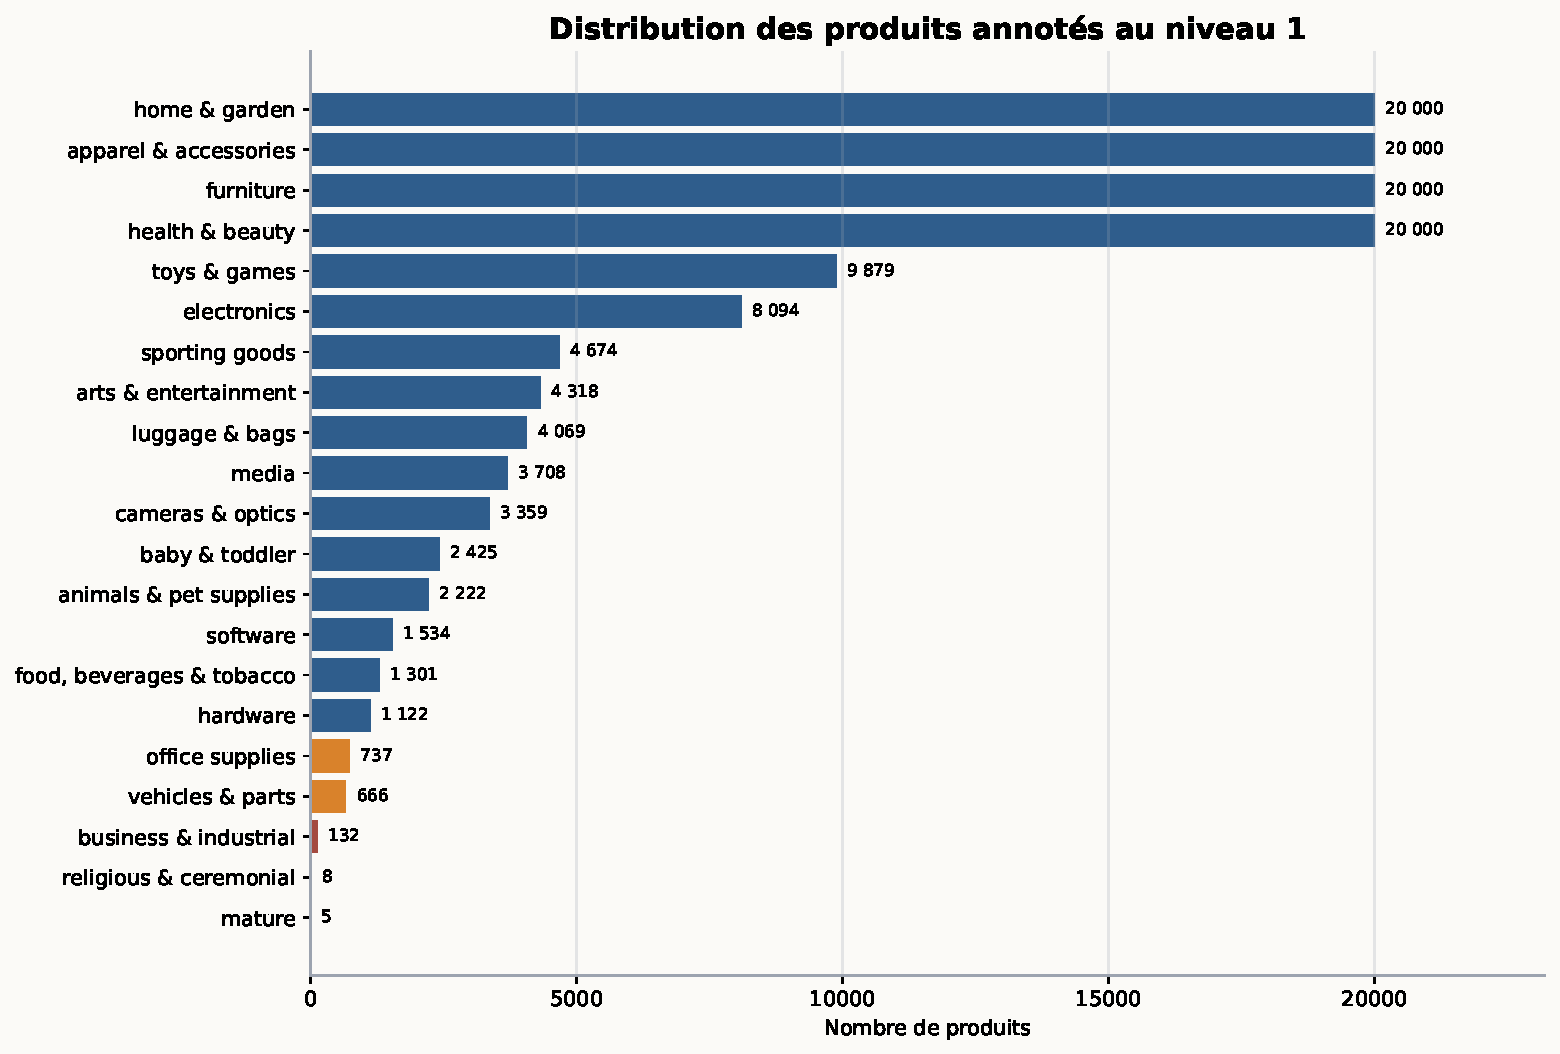
\includegraphics[width=0.92\textwidth]{figures/dataset_l1_distribution.pdf}
    \caption{Distribution des produits annotés au Niveau 1.}
    \label{fig:distL1}
\end{figure}

\begin{figure}[H]
    \centering
    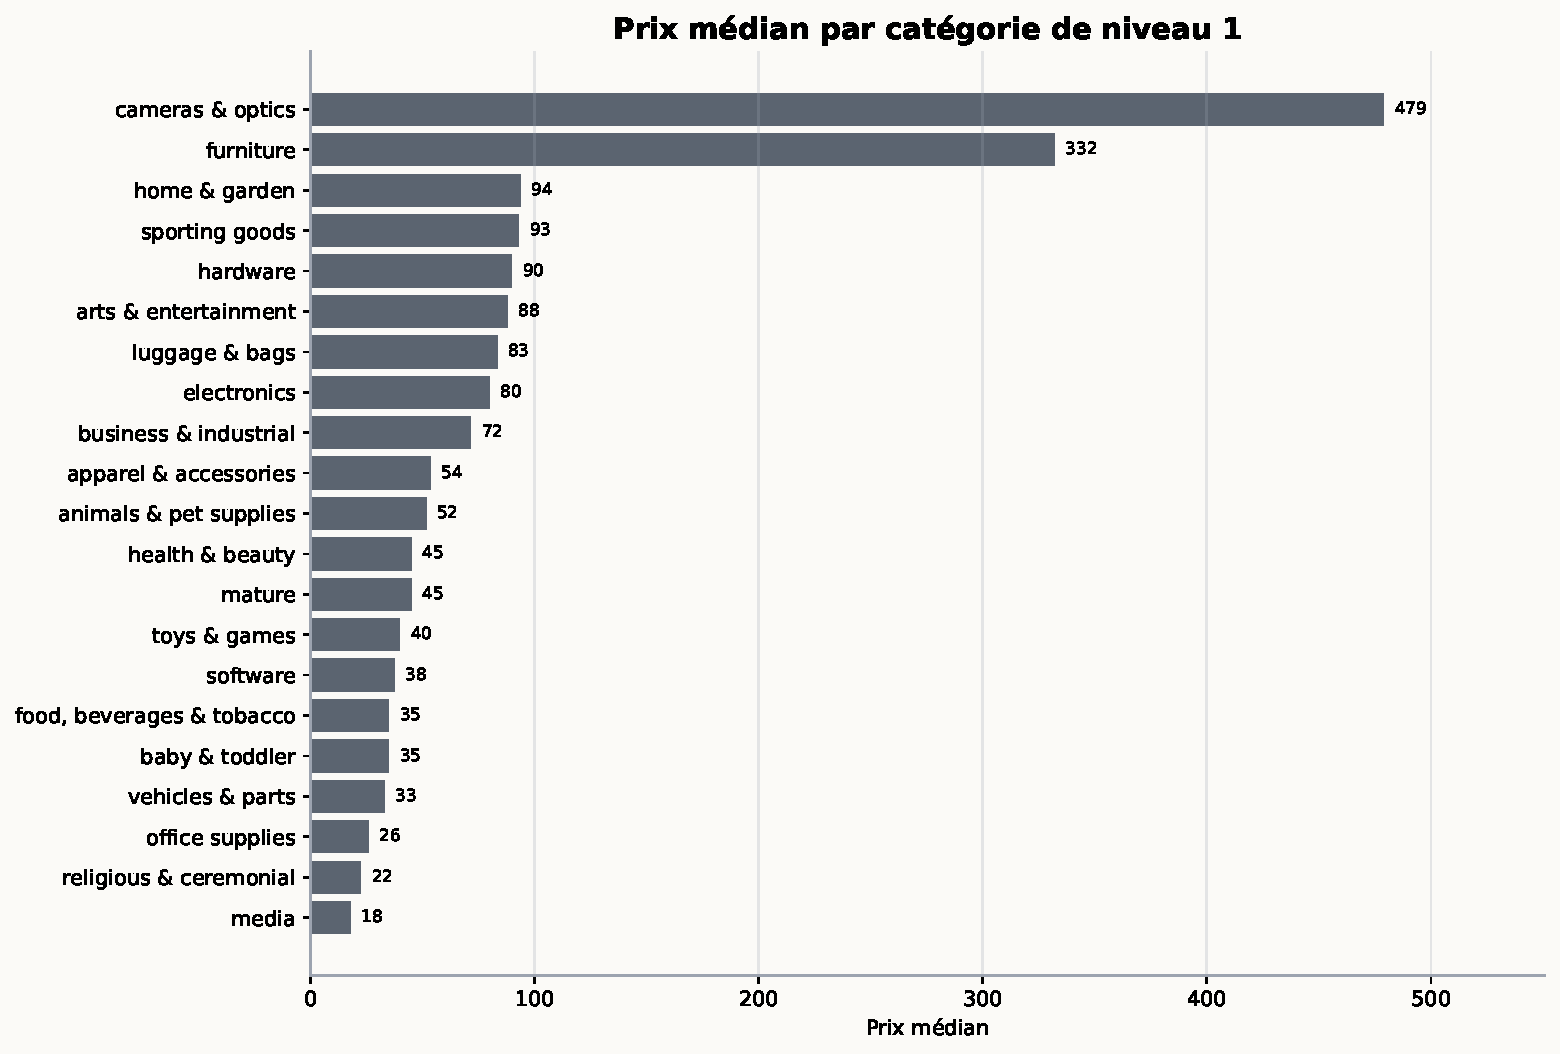
\includegraphics[width=0.48\textwidth]{figures/dataset_l1_median_price.pdf}
    \hfill
    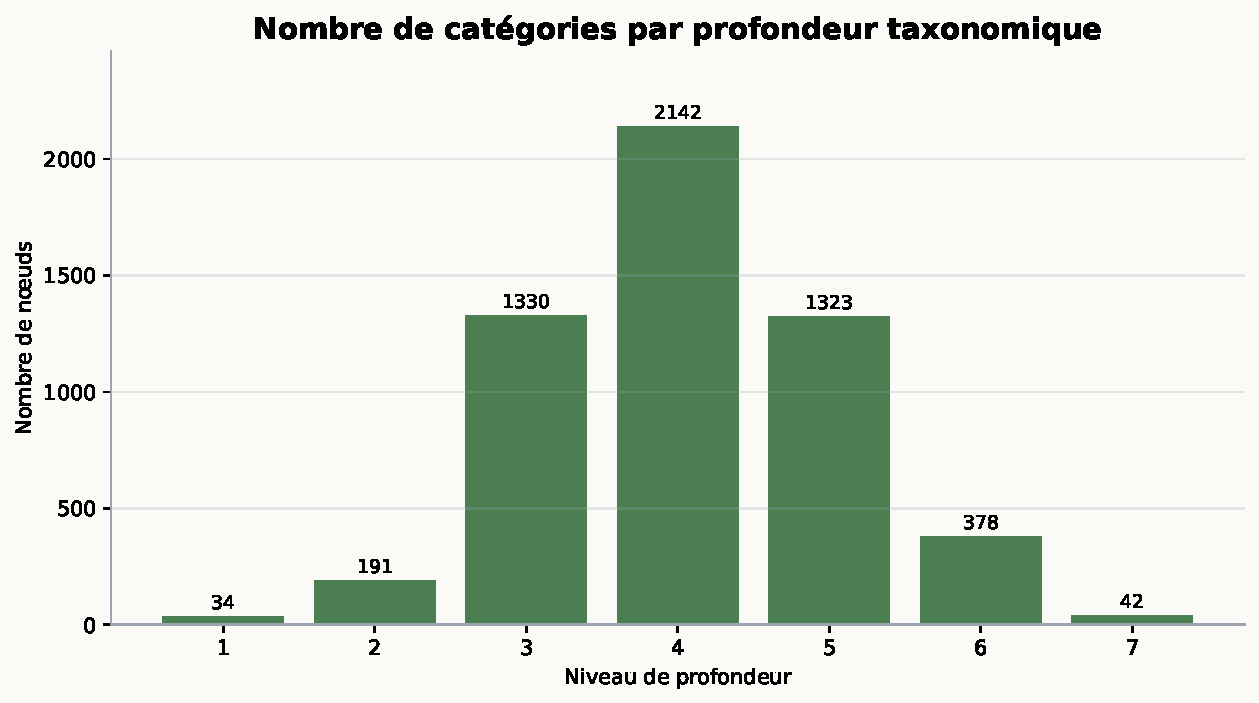
\includegraphics[width=0.48\textwidth]{figures/taxonomy_depth_distribution.pdf}
    \caption{Prix médian par catégorie L1, à gauche, et distribution de profondeur de la taxonomie, à droite.}
    \label{fig:data-price-taxonomy-depth-annex}
\end{figure}

\begin{figure}[H]
    \centering
    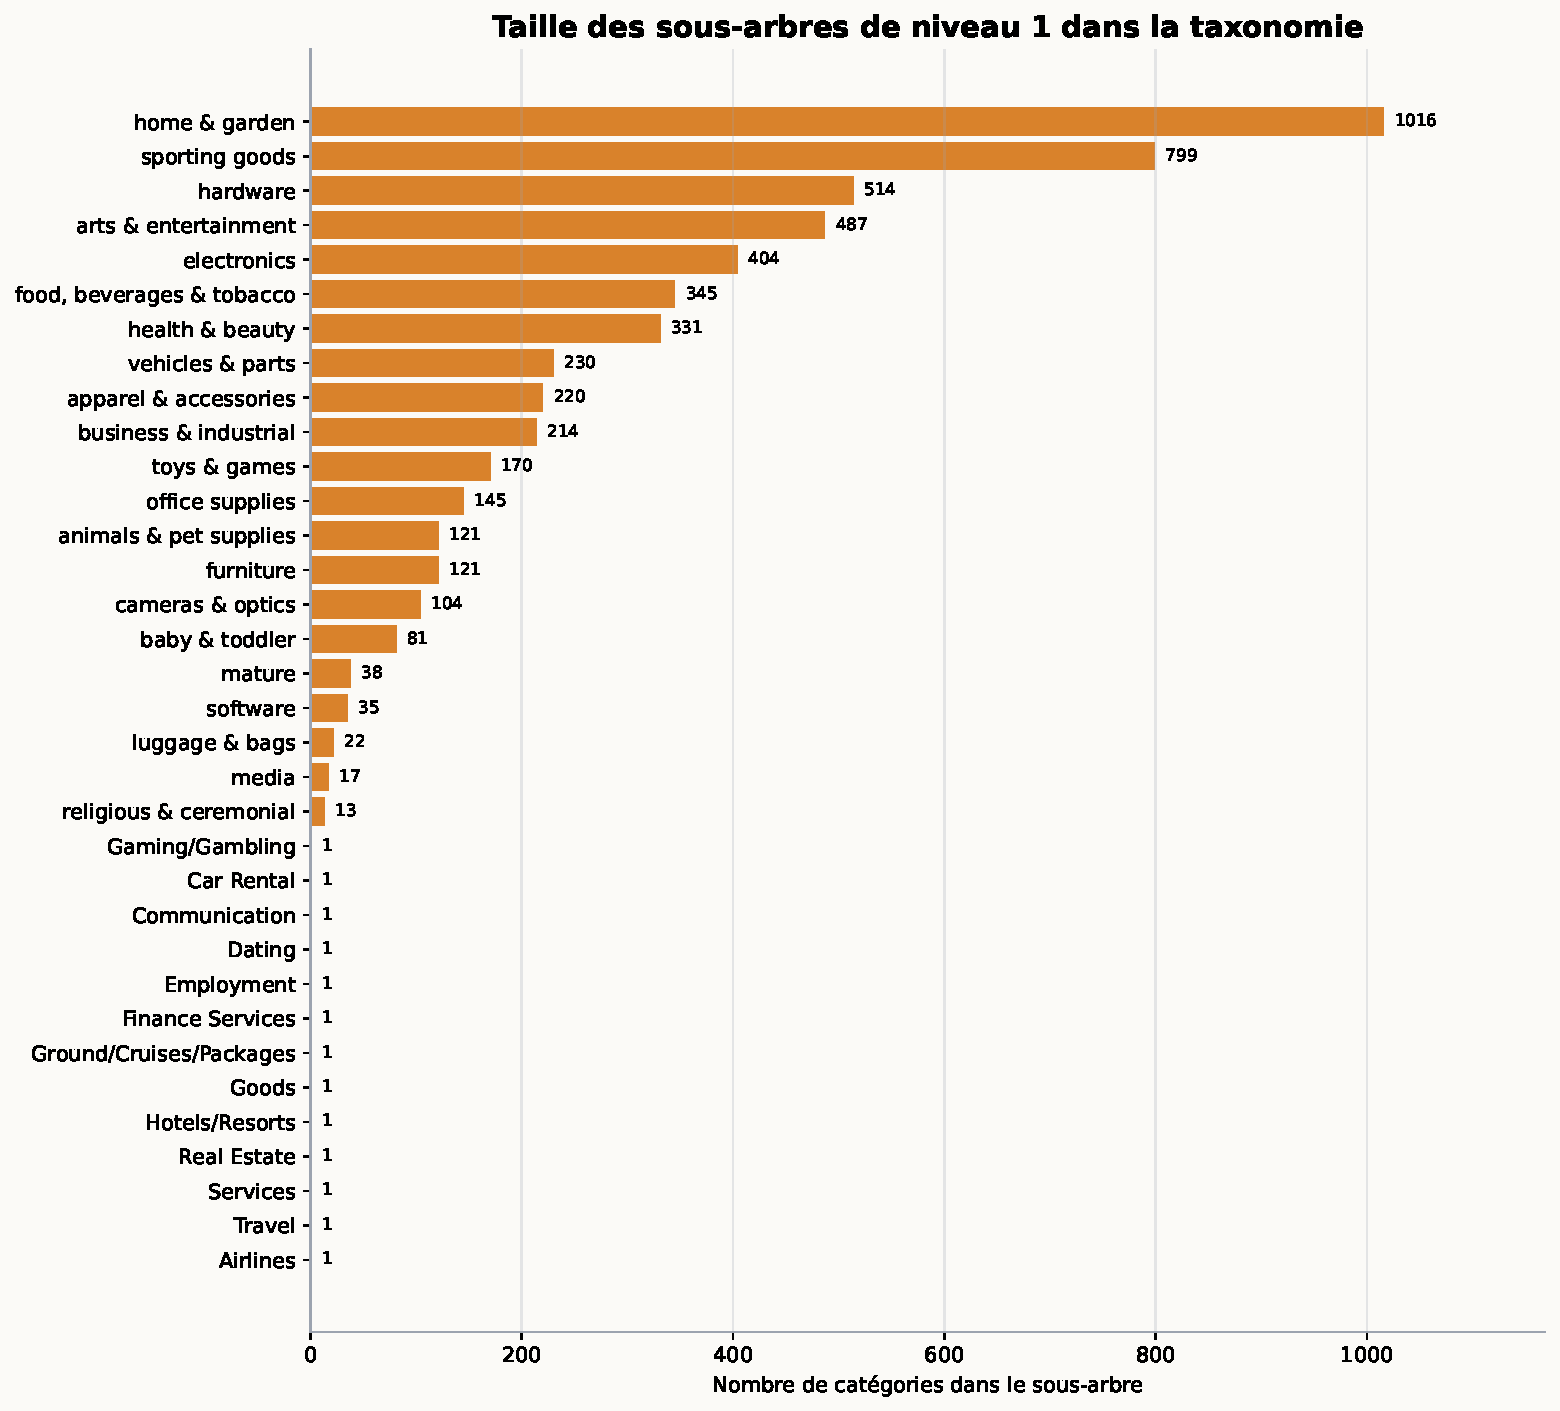
\includegraphics[width=0.48\textwidth]{figures/taxonomy_l1_branch_sizes.pdf}
    \hfill
    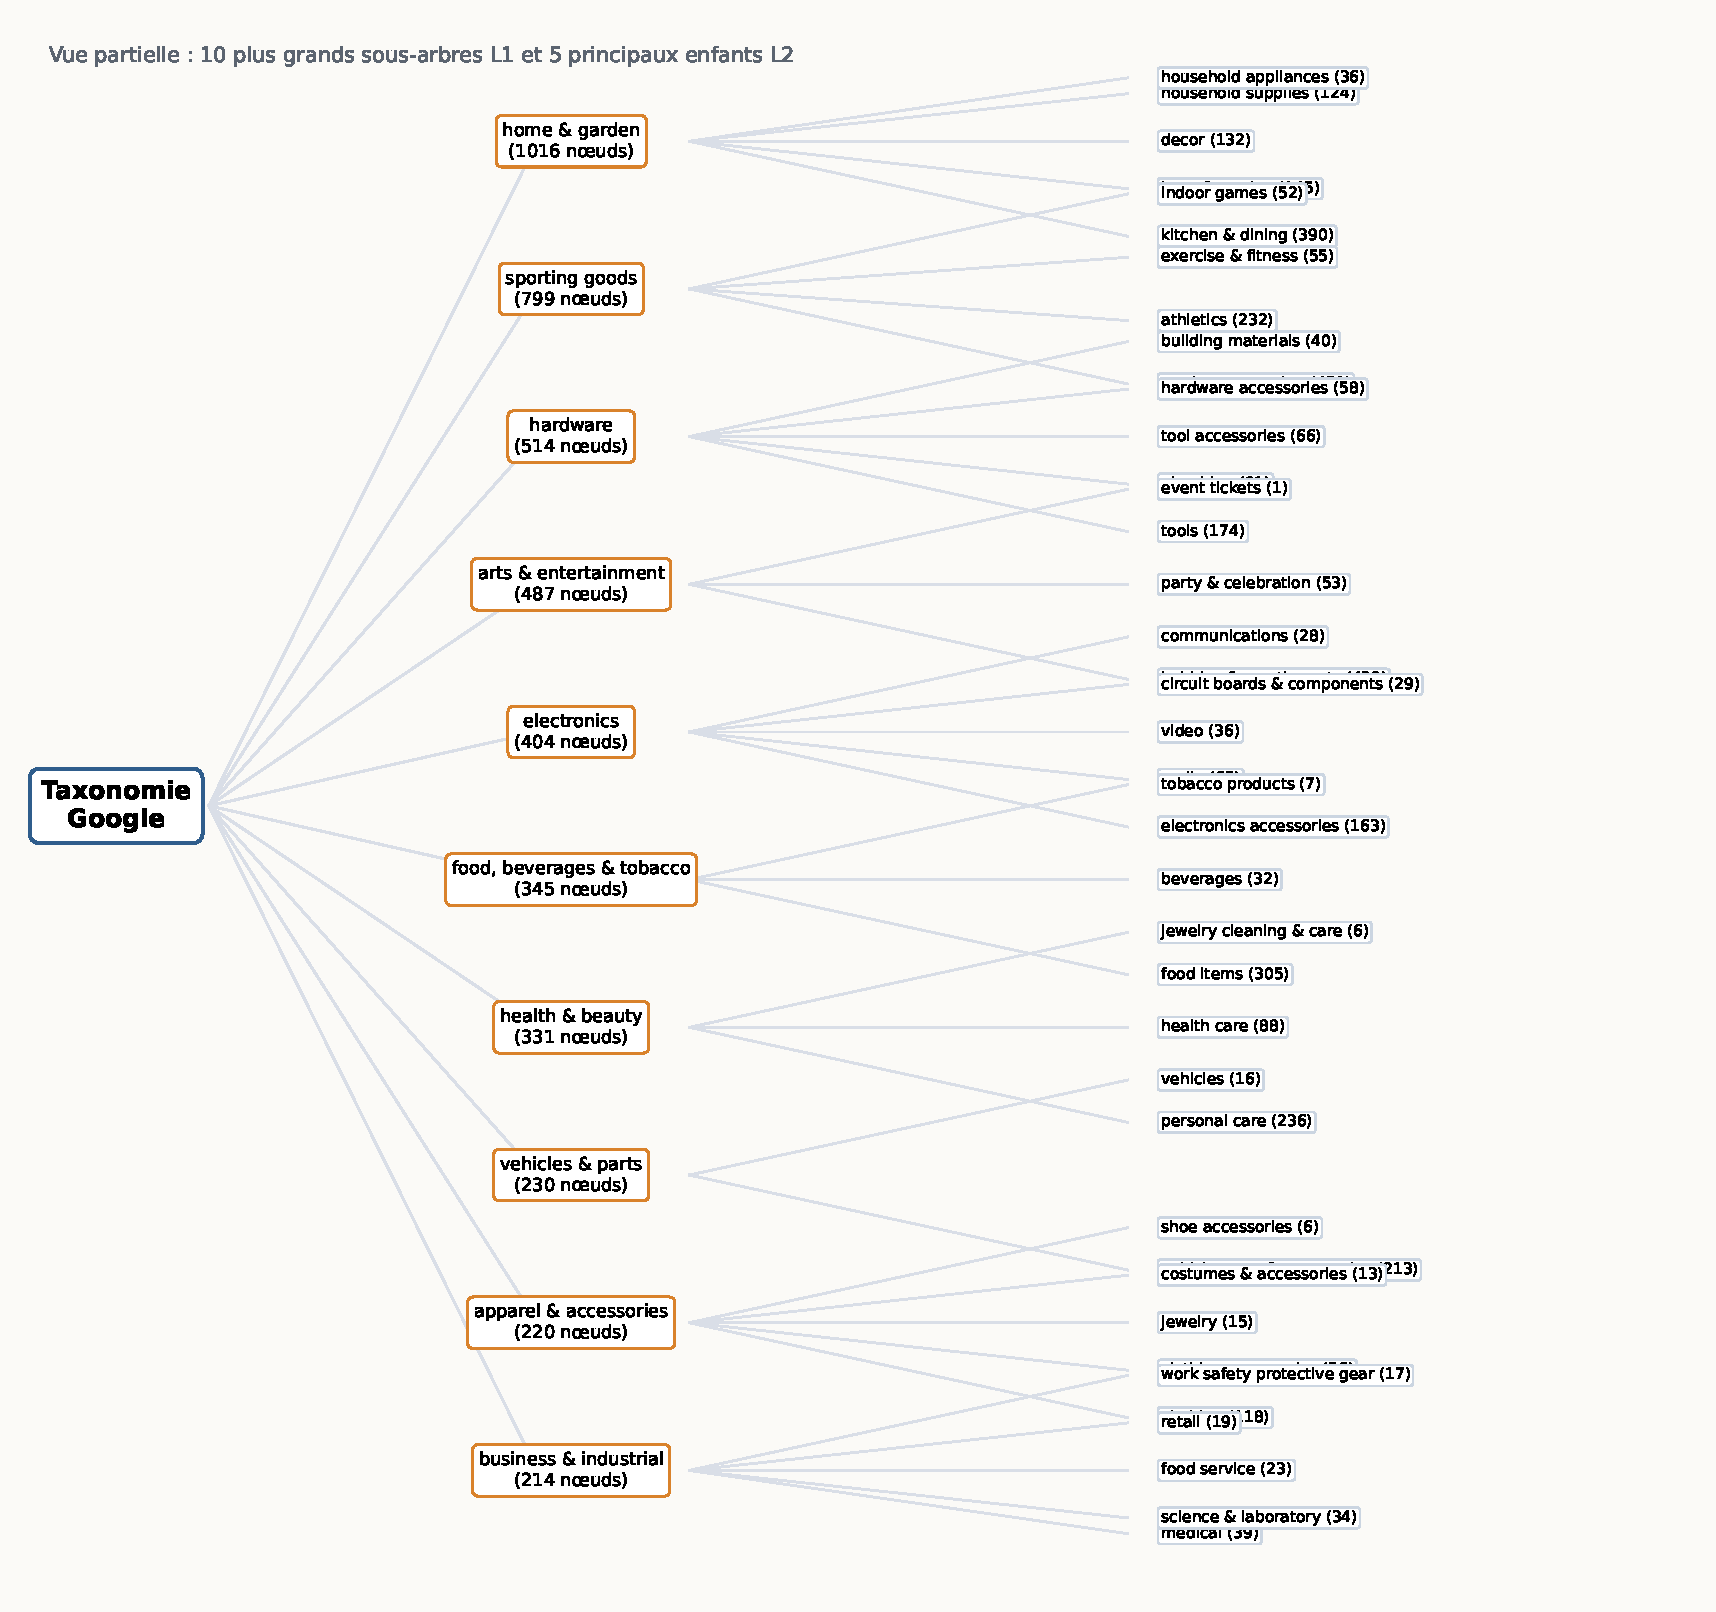
\includegraphics[width=0.48\textwidth]{figures/taxonomy_l1_l2_tree.pdf}
    \caption{Tailles des branches L1 et visualisation partielle de l'arbre L1--L2.}
    \label{fig:data-taxonomy-tree-annex}
\end{figure}

\section*{Définition des métriques de classification L1}
\label{sec:l1-classification-metrics-annex}

\noindent\hyperref[sec:l1-final-metrics]{Retour vers les métriques finales du modèle L1.}

Cette annexe détaille les métriques utilisées dans le tableau \ref{tab:l1-final-classification-metrics}. On considère un problème de classification à $K$ catégories de Niveau 1. Pour une catégorie $k$, on note $TP_k$ les vrais positifs, $FP_k$ les faux positifs, $FN_k$ les faux négatifs et $n_k$ le nombre d'exemples de cette catégorie dans l'ensemble de test. Le nombre total de produits évalués est $N=\sum_{k=1}^{K} n_k$.

\paragraph{accuracy top-1.}
L'accuracy top-1 mesure la proportion de produits pour lesquels la première catégorie prédite est exactement la catégorie vraie :
\begin{equation}
    \operatorname{Acc@1}
    =
    \frac{1}{N}
    \sum_{i=1}^{N}
    \mathbf{1}\left[\hat{y}_i^{(1)}=y_i\right].
\end{equation}
Dans notre cadre mono-label, l'accuracy top-1 est égale au micro-$F_1$, car chaque produit reçoit exactement une prédiction.

\paragraph{accuracy top-$k$.}
L'accuracy top-$k$ vérifie si le label vrai apparaît dans les $k$ meilleures catégories proposées par le modèle :
\begin{equation}
    \operatorname{Acc@}k
    =
    \frac{1}{N}
    \sum_{i=1}^{N}
    \mathbf{1}\left[y_i \in \{\hat{y}_i^{(1)},\ldots,\hat{y}_i^{(k)}\}\right].
\end{equation}
Cette métrique est utile pour mesurer si la bonne catégorie reste proche dans l'espace d'embeddings même lorsque le top-1 est incorrect.

\paragraph{Precision, recall et $F_1$ par classe.}
Pour chaque catégorie $k$, la précision et le recall sont définis par :
\begin{equation}
    P_k
    =
    \frac{TP_k}{TP_k+FP_k},
    \qquad
    R_k
    =
    \frac{TP_k}{TP_k+FN_k}.
\end{equation}
La précision mesure la fiabilité des prédictions faites vers la classe $k$ ; le recall mesure la capacité à retrouver les produits appartenant réellement à $k$. Le $F_1$ score combine les deux par moyenne harmonique :
\begin{equation}
    F_{1,k}
    =
    \frac{2P_kR_k}{P_k+R_k}.
\end{equation}

\paragraph{Macro-précision, macro-recall et macro-$F_1$.}
Les macro-métriques donnent le même poids à chaque catégorie, indépendamment de sa fréquence :
\begin{equation}
    \operatorname{MacroPrecision}
    =
    \frac{1}{K}\sum_{k=1}^{K}P_k,
    \qquad
    \operatorname{MacroRecall}
    =
    \frac{1}{K}\sum_{k=1}^{K}R_k,
\end{equation}
\begin{equation}
    \operatorname{MacroF_1}
    =
    \frac{1}{K}\sum_{k=1}^{K}F_{1,k}.
\end{equation}
Ces métriques sont centrales dans notre cas, car la distribution des catégories L1 est déséquilibrée. Une bonne micro-accuracy peut masquer de mauvaises performances sur les catégories rares, alors qu'une macro-métrique les rend visibles.

\paragraph{accuracy équilibrée.}
L'accuracy équilibrée correspond à la moyenne des recalls par classe. Dans un problème multi-classe, elle est donc équivalente au macro-recall :
\begin{equation}
    \operatorname{BalancedAccuracy}
    =
    \frac{1}{K}\sum_{k=1}^{K}
    \frac{TP_k}{TP_k+FN_k}.
\end{equation}
Elle indique si le modèle retrouve correctement chaque catégorie, sans laisser les classes fréquentes dominer l'évaluation.

\paragraph{$F_1$ pondéré.}
Le $F_1$ pondéré pondère le $F_1$ de chaque catégorie par son support $n_k$ :
\begin{equation}
    \operatorname{WeightedF_1}
    =
    \sum_{k=1}^{K}
    \frac{n_k}{N}
    F_{1,k}.
\end{equation}
Cette métrique reflète mieux la performance globale sur le catalogue réel, car les grandes catégories contribuent davantage. Elle doit cependant être lue avec les macro-métriques : un $F_1$ pondéré élevé peut rester compatible avec des erreurs importantes sur des catégories rares.

\paragraph{Lecture conjointe des métriques.}
Dans le rapport, nous retenons le modèle L1 parce qu'il combine une accuracy top-1 élevée, une accuracy top-5 très élevée et un macro-recall nettement amélioré par l'échantillonnage tempéré. La micro-accuracy mesure la qualité globale sur le catalogue, tandis que les macro-métriques vérifient que l'amélioration ne se fait pas au détriment des catégories peu représentées.

\section*{Projection UMAP et comparaison PCA des embeddings de Niveau 1}
\label{sec:umap-pca-annex}

\noindent\hyperref[chap:l1-supervised]{Retour vers le chapitre de modélisation supervisée L1.}

UMAP construit un graphe de voisinage local dans l'espace original, puis optimise une représentation de faible dimension qui conserve au mieux ces voisinages. Ce choix est cohérent avec l'intuition développée dans le rapport : dans l'espace d'embeddings, les catégories ne forment pas nécessairement des nuages linéaires, mais plutôt des régions ou variétés sémantiques locales. UMAP est donc plus adapté qu'une projection purement linéaire lorsque la structure pertinente est locale et non linéaire.

La projection UMAP est uniquement utilisée comme outil d'inspection qualitative de l'espace latent. Les distances exactes observées en deux dimensions ne doivent pas être interprétées comme des distances de classification, car elles résultent d'une projection compressive depuis un espace d'embeddings de dimension beaucoup plus élevée.

La figure \ref{fig:l1-embedding-pca-annex} présente la même matrice d'embeddings que la projection UMAP du \hyperref[chap:l1-supervised]{chapitre principal}, mais projetée avec PCA. Cette visualisation est conservée comme point de comparaison méthodologique : PCA cherche les directions linéaires de variance maximale, alors que UMAP cherche à préserver les voisinages locaux. Dans notre cas, la PCA donne une séparation moins exploitable visuellement, ce qui confirme que la structure apprise par fine-tuning est mieux décrite par une géométrie locale non linéaire que par deux axes linéaires globaux.

\begin{figure}[H]
    \centering
    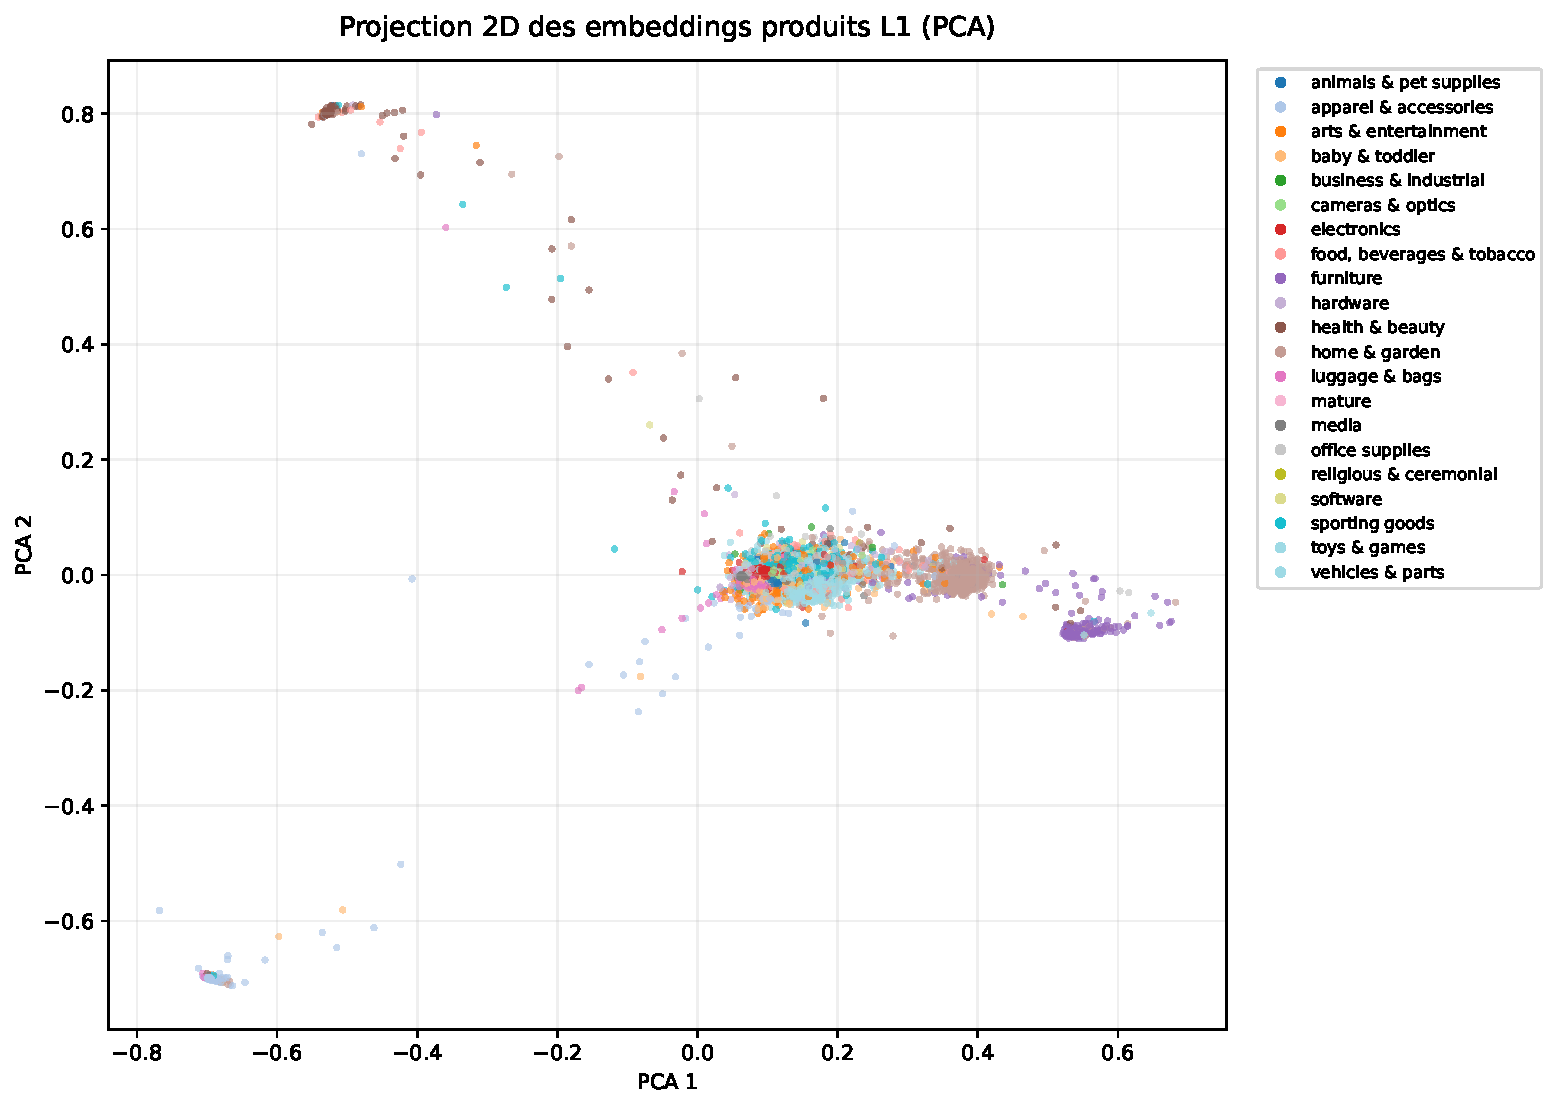
\includegraphics[width=0.95\textwidth]{figures/l1_embedding_projection_pca.pdf}
    \caption{Projection PCA des embeddings produits après fine-tuning supervisé du Niveau 1.}
    \label{fig:l1-embedding-pca-annex}
\end{figure}

\section*{V de Cramér pour l'association entre pipelines}
\label{sec:cramers-v-annex}

\noindent\hyperref[sec:l2-l7-unsupervised-metrics]{Retour vers la méthodologie des métriques non supervisées.}

Dans la comparaison des pipelines L2--L7, chaque méthode produit un label discret : un chemin taxonomique complet, ou un label à un niveau donné. Une corrélation de Pearson n'est pas adaptée à ce cas, car elle suppose des variables numériques ordonnées. Or deux chemins taxonomiques sont des catégories nominales : leur identifiant numérique éventuel n'a pas de sens métrique.

Le V de Cramér mesure l'intensité de l'association entre deux variables catégorielles. Supposons que deux pipelines $A$ et $B$ produisent respectivement des labels dans $\{a_1,\ldots,a_r\}$ et $\{b_1,\ldots,b_c\}$. On construit la table de contingence :
\begin{equation}
    N =
    \left(n_{ij}\right)_{1 \leq i \leq r,\ 1 \leq j \leq c},
    \qquad
    n_{ij}
    =
    \#\left\{x : A(x)=a_i,\ B(x)=b_j\right\}.
\end{equation}
On note $n=\sum_{i=1}^{r}\sum_{j=1}^{c} n_{ij}$ le nombre total de produits comparés, $n_{i\cdot}=\sum_{j=1}^{c}n_{ij}$ les marges lignes et $n_{\cdot j}=\sum_{i=1}^{r}n_{ij}$ les marges colonnes. Sous l'hypothèse d'indépendance entre les deux pipelines, l'effectif attendu dans la cellule $(i,j)$ est :
\begin{equation}
    e_{ij}
    =
    \frac{n_{i\cdot}n_{\cdot j}}{n}.
\end{equation}
La statistique du chi-deux associée à la table est alors :
\begin{equation}
    \chi^2
    =
    \sum_{i=1}^{r}\sum_{j=1}^{c}
    \frac{(n_{ij}-e_{ij})^2}{e_{ij}}.
\end{equation}
Le V de Cramér normalise cette quantité afin d'obtenir une mesure comprise entre 0 et 1 :
\begin{equation}
    V
    =
    \sqrt{
    \frac{\chi^2}
    {n \cdot \min(r-1,c-1)}
    }.
\end{equation}

L'interprétation est la suivante. Une valeur proche de 0 indique que les prédictions des deux pipelines sont faiblement associées : connaître le label prédit par le premier pipeline informe peu sur le label prédit par le second. Une valeur proche de 1 indique une forte association catégorielle : les labels produits par un pipeline contraignent fortement ceux de l'autre. Cette notion est différente de l'accord exact. Deux pipelines peuvent avoir un accord exact faible mais un V de Cramér élevé si leurs prédictions sont liées par une correspondance régulière entre catégories. Par exemple, un pipeline peut systématiquement choisir une catégorie plus générale tandis qu'un autre choisit une sous-branche proche ; les labels ne sont pas identiques, mais la relation statistique reste forte.

Dans notre contexte non supervisé, cette propriété est utile pour distinguer deux situations. Si l'accord exact et le V de Cramér sont élevés, les pipelines produisent presque les mêmes chemins. Si l'accord exact est faible mais le V de Cramér reste élevé, les pipelines divergent localement mais capturent une structure catégorielle commune. Si les deux sont faibles, les méthodes produisent des hypothèses réellement différentes, ce qui signale des produits ou des branches à auditer en priorité.

Le V de Cramér présente donc trois avantages pour notre comparaison. Premièrement, il respecte la nature nominale des prédictions taxonomiques. Deuxièmement, il est normalisé entre 0 et 1, ce qui facilite la comparaison entre paires de pipelines. Troisièmement, il mesure une association globale entre distributions de labels, pas seulement une égalité stricte produit par produit.

Il faut toutefois rappeler ses limites. Le V de Cramér n'est pas une mesure d'accuracy : sans vérité terrain L2--L7, une forte association entre deux pipelines ne prouve pas que leurs prédictions sont correctes. Il est aussi sensible aux tables très creuses, fréquentes lorsque le nombre de chemins distincts est élevé. Pour cette raison, nous l'utilisons conjointement avec l'accord exact, l'accord niveau par niveau, les marges de confiance, la diversité des chemins et les scores sémantiques externes.

\section*{Tableau global des métriques L2--L7 non supervisées}
\label{sec:l2-l7-metrics-annex}

\noindent\hyperref[sec:l2-l7-unsupervised-metrics]{Retour vers la méthodologie des métriques non supervisées.}

Le tableau \ref{tab:l2-l7-global-metrics-annex} synthétise les trois familles de métriques utilisées pour comparer les pipelines L2--L7. Ces indicateurs ne remplacent pas une accuracy supervisée ; ils servent à comparer le coût, la stabilité et la cohérence relative des méthodes en l'absence de vérité terrain.

\begin{table}[H]
    \centering
    \caption{Synthèse des métriques non supervisées utilisées pour comparer les pipelines L2--L7.}
    \label{tab:l2-l7-global-metrics-annex}
    \scriptsize
    \resizebox{\textwidth}{!}{%
    \begin{tabular}{p{3.0cm}p{3.2cm}p{5.0cm}p{5.4cm}}
        \toprule
        \textbf{Famille} & \textbf{Métrique} & \textbf{Interprétation} & \textbf{Lecture dans nos expériences} \\
        \midrule
        Coût d'inférence & Temps moyen par produit & Mesure la latence opérationnelle du pipeline une fois les embeddings disponibles. Plus la valeur est faible, plus la méthode est compatible avec un passage à l'échelle. & Le clustering et le greedy sont les plus rapides. Le beam augmente le temps car il conserve plusieurs chemins. Le beam + reranker est le plus coûteux et doit être réservé aux cas incertains. \\
        Coût d'inférence & Millions d'opérations par produit & Approxime le nombre de produits scalaires entre embeddings. Cette métrique dépend directement du nombre de candidats comparés et de la dimension de l'encodeur. & Qwen3 est avantagé car sa dimension est 1024, contre 2048 pour Jasper. À stratégie identique, Jasper double approximativement le coût vectoriel. \\
        Coût d'inférence & Mémoire chargée & Mesure la taille des matrices nécessaires en inférence : produits, prototypes ou chemins globaux. & Qwen3 occupe environ 651 MB pour les embeddings partagés, contre 1{,}3 GB pour Jasper. Qwen3 est donc plus favorable si la contrainte principale est la mémoire d'inférence. \\
        Confiance interne & Marge top-1/top-2 & Mesure l'écart entre le meilleur candidat et le second. Une marge faible indique une décision instable. & Le beam explore davantage mais conserve souvent des marges faibles, surtout avec Qwen3. Le clustering a une marge médiane plus élevée, car l'affectation centroïde--catégorie est parfois plus nette. \\
        Confiance interne & Profondeur moyenne prédite & Indique jusqu'où la méthode descend dans la taxonomie. Une profondeur élevée n'est positive que si elle reste associée à une confiance suffisante. & La recherche de chemins globaux descend généralement plus profondément. Le clustering est plus prudent et tend à produire des chemins légèrement moins profonds. \\
        Confiance interne & Diversité et concentration des chemins & Combine le nombre de chemins distincts, l'entropie et la part du chemin le plus fréquent. Une forte concentration peut signaler un biais vers des chemins génériques. & Qwen3 produit des chemins plus diversifiés. Jasper donne des scores cosinus plus forts mais concentre davantage les prédictions sur quelques chemins, sauf avec reranker ou clustering. \\
        Comparaison entre pipelines & Accord exact sur le chemin & Mesure la proportion de produits pour lesquels deux pipelines prédisent exactement le même chemin. & Greedy et beam sont les plus proches. Le clustering est volontairement plus différent, car il exploite la structure collective des produits plutôt qu'une décision locale. \\
        Comparaison entre pipelines & Accord niveau par niveau L2--L7 & Localise le premier niveau où les pipelines divergent. Cette métrique est plus informative qu'un accord complet lorsque les chemins sont profonds. & Les pipelines peuvent être cohérents en L2 mais diverger ensuite. Cela montre que la difficulté principale se situe souvent dans les niveaux profonds. \\
        Comparaison entre pipelines & V de Cramér & Mesure l'association statistique entre deux distributions de labels discrets, même lorsque les labels ne sont pas strictement identiques. & Un V élevé avec un accord faible signifie que les pipelines suivent une structure catégorielle commune mais choisissent des chemins différents. Cette situation identifie des branches à auditer plutôt qu'un échec direct. \\
        Comparaison entre pipelines & Score NLP externe et taux de victoire & Compare les chemins concurrents d'un même produit avec un modèle de ranking ou de similarité sémantique. & La recherche de chemins globaux obtient le meilleur score moyen sur l'audit Qwen3, tandis que le greedy reste compétitif en taux de victoire. Cela suggère une possible règle hybride selon la branche L1 et la marge. \\
        \bottomrule
    \end{tabular}
    }
\end{table}

\section*{Matrices d'accord L2--L7 et vitesse de divergence}
\label{sec:l2-l7-family3-matrices-annex}

\noindent\hyperref[sec:l2-l7-pipeline-agreement]{Retour vers la comparaison des pipelines entre eux.}

Cette annexe complète la comparaison famille 3 en visualisant les matrices d'accord exact niveau par niveau. Pour un niveau $\ell \in \{2,\ldots,7\}$ et deux pipelines $A$ et $B$, l'accord reporté dans la matrice est :
\begin{equation}
    \operatorname{Acc}_{\ell}(A,B)
    =
    \frac{1}{n_{\ell}}
    \sum_{i=1}^{n_{\ell}}
    \mathbf{1}\left[
    \hat{y}^{A}_{i,\ell}
    =
    \hat{y}^{B}_{i,\ell}
    \right],
\end{equation}
où $n_{\ell}$ désigne le nombre de produits pour lesquels au moins l'un des deux pipelines prédit un label au niveau $\ell$. Cette définition permet de comparer les pipelines uniquement sur les niveaux effectivement atteints.

La divergence associée est définie par :
\begin{equation}
    \operatorname{Div}_{\ell}(A,B)
    =
    1
    -
    \operatorname{Acc}_{\ell}(A,B).
\end{equation}
Elle mesure donc la vitesse à laquelle deux pipelines cessent de prédire les mêmes catégories quand on descend dans la taxonomie. Une divergence faible en L2 mais forte en L4 signifie que les méthodes s'accordent sur la grande famille de produits, mais choisissent rapidement des sous-branches différentes.

\begin{figure}[H]
    \centering
    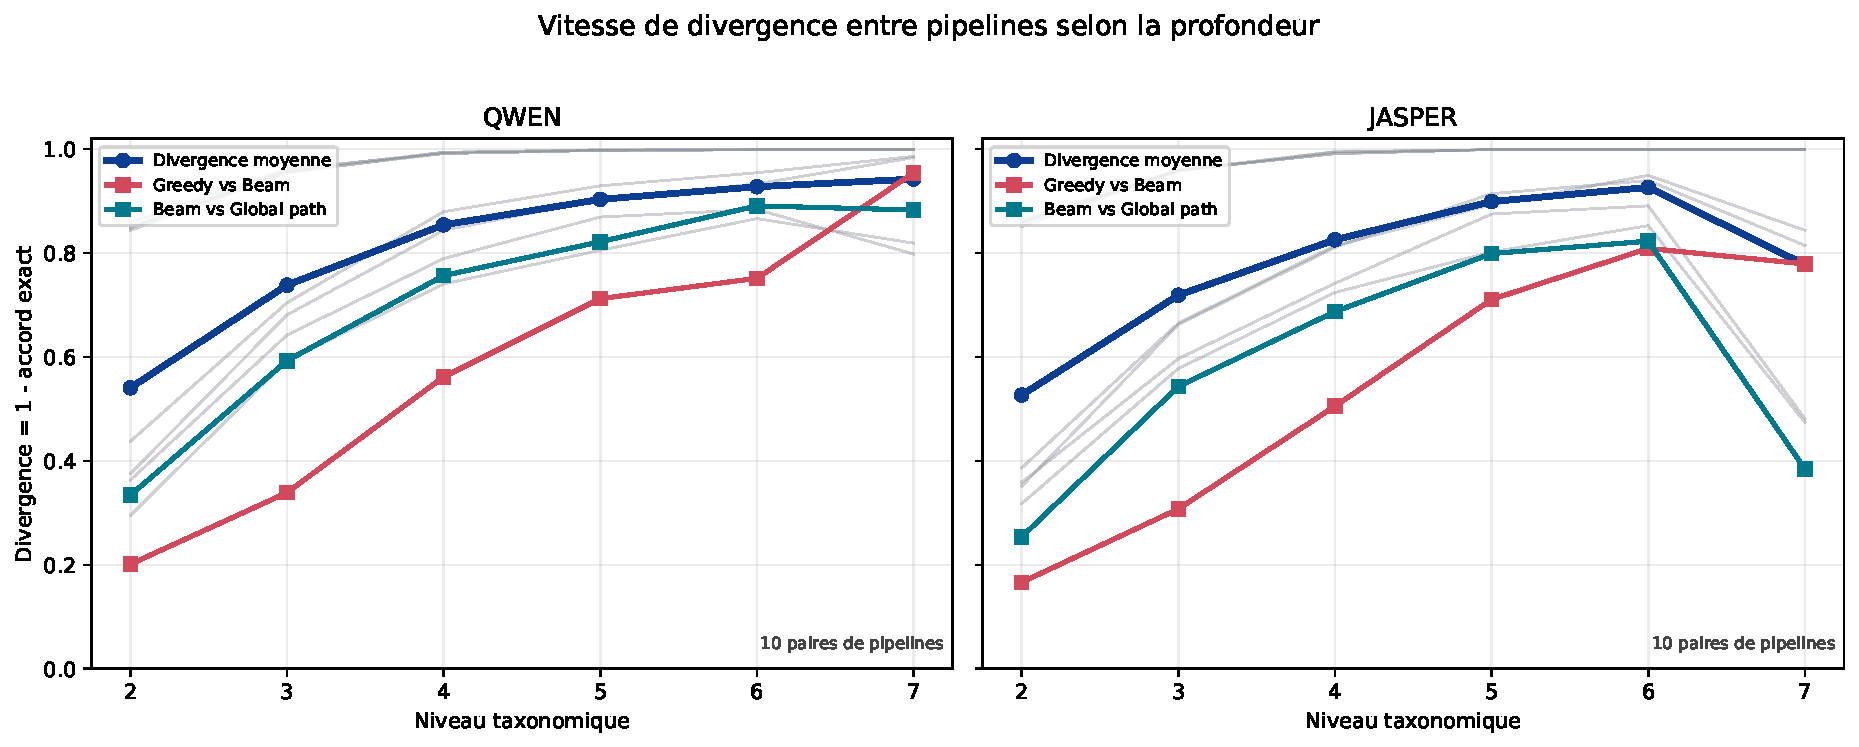
\includegraphics[width=0.98\textwidth]{figures/l2_l7_family3_annex/family3_divergence_by_depth.pdf}
    \caption{Vitesse de divergence entre pipelines selon la profondeur taxonomique. Les courbes grises correspondent aux paires de pipelines ; la courbe bleue indique la divergence moyenne.}
    \label{fig:l2-l7-family3-divergence-depth}
\end{figure}

La figure \ref{fig:l2-l7-family3-divergence-depth} montre que la divergence augmente très rapidement entre L2 et L4. Cette observation confirme que les premières décisions hiérarchiques restent relativement partagées entre certaines méthodes, en particulier greedy et beam, mais que les chemins se différencient fortement dès que la taxonomie devient plus fine. Les niveaux L6--L7 doivent être interprétés avec prudence : peu de produits atteignent ces profondeurs, ce qui rend les accords plus sensibles à la taille des sous-échantillons.

\begin{figure}[H]
    \centering
    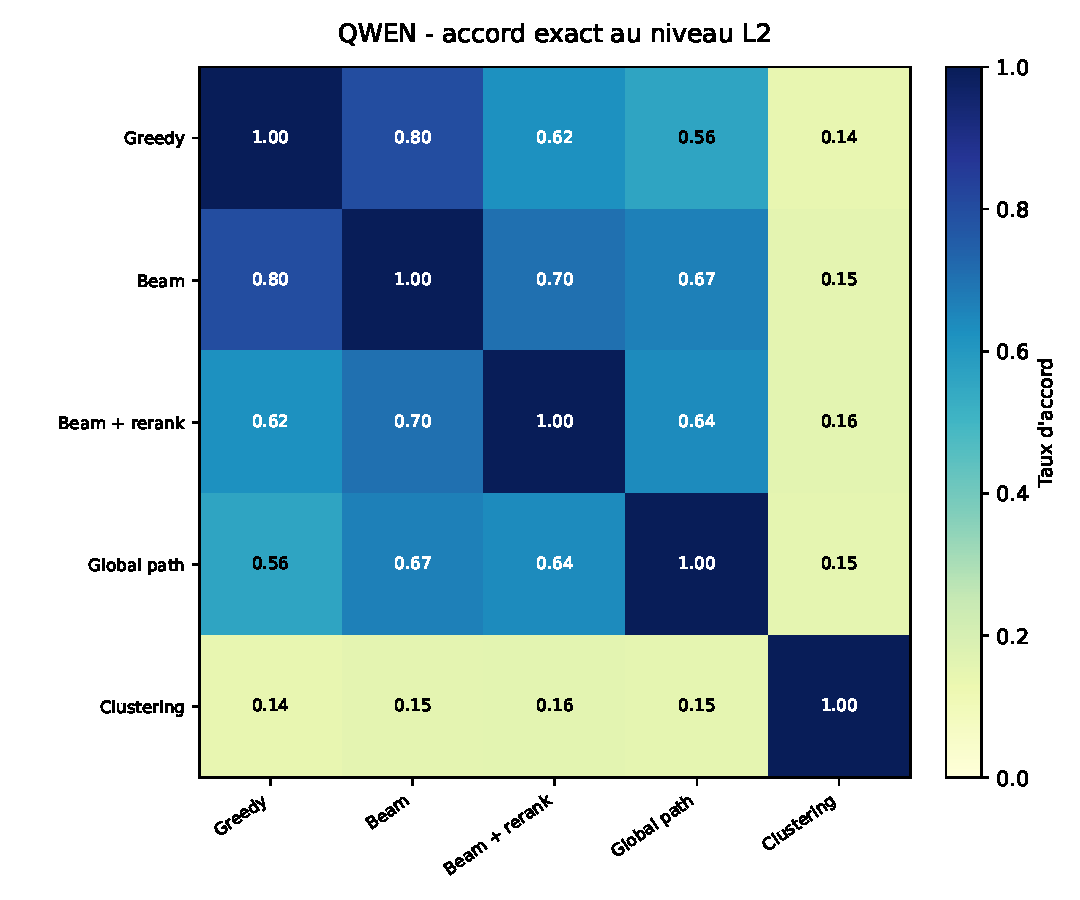
\includegraphics[width=0.48\textwidth]{figures/l2_l7_family3_annex/family3_qwen_level_2_agreement_heatmap.pdf}
    \hfill
    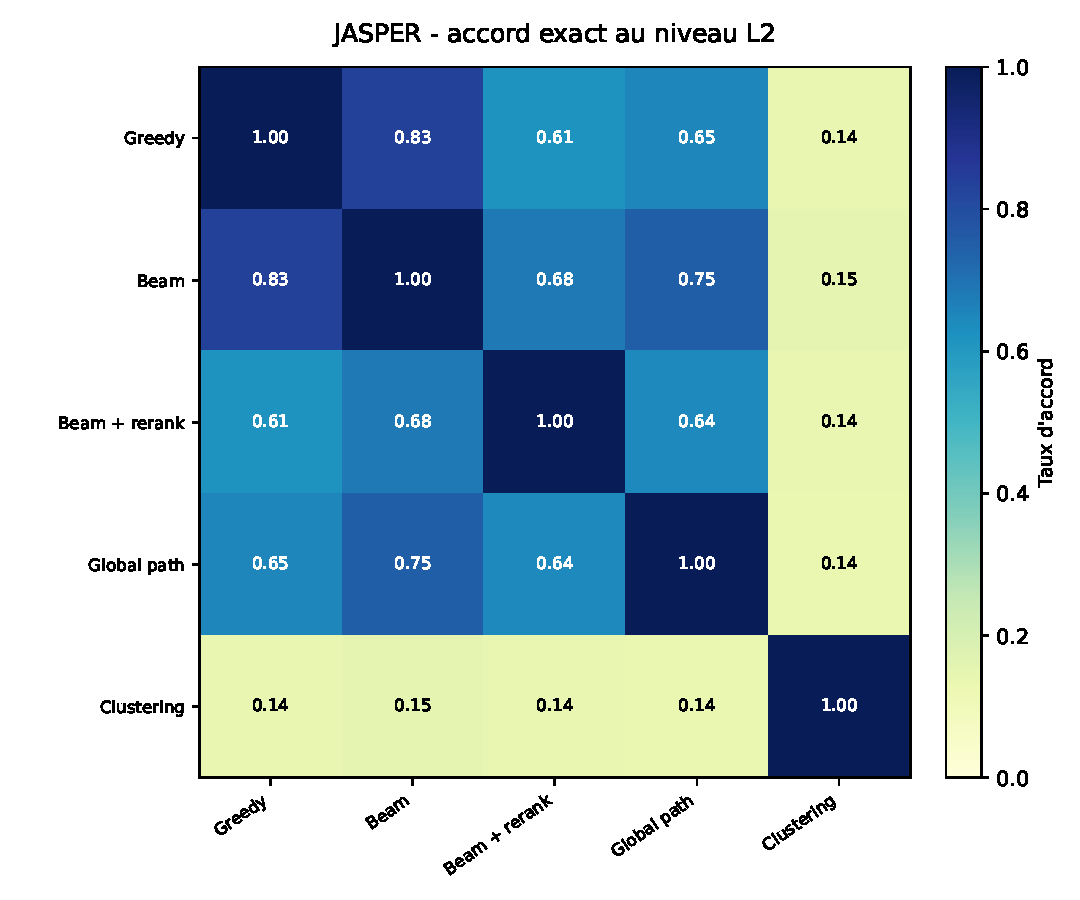
\includegraphics[width=0.48\textwidth]{figures/l2_l7_family3_annex/family3_jasper_level_2_agreement_heatmap.pdf}
    \caption{Matrices d'accord exact au Niveau 2 pour Qwen3, à gauche, et Jasper, à droite.}
    \label{fig:l2-l7-family3-level2-matrix}
\end{figure}

\begin{figure}[H]
    \centering
    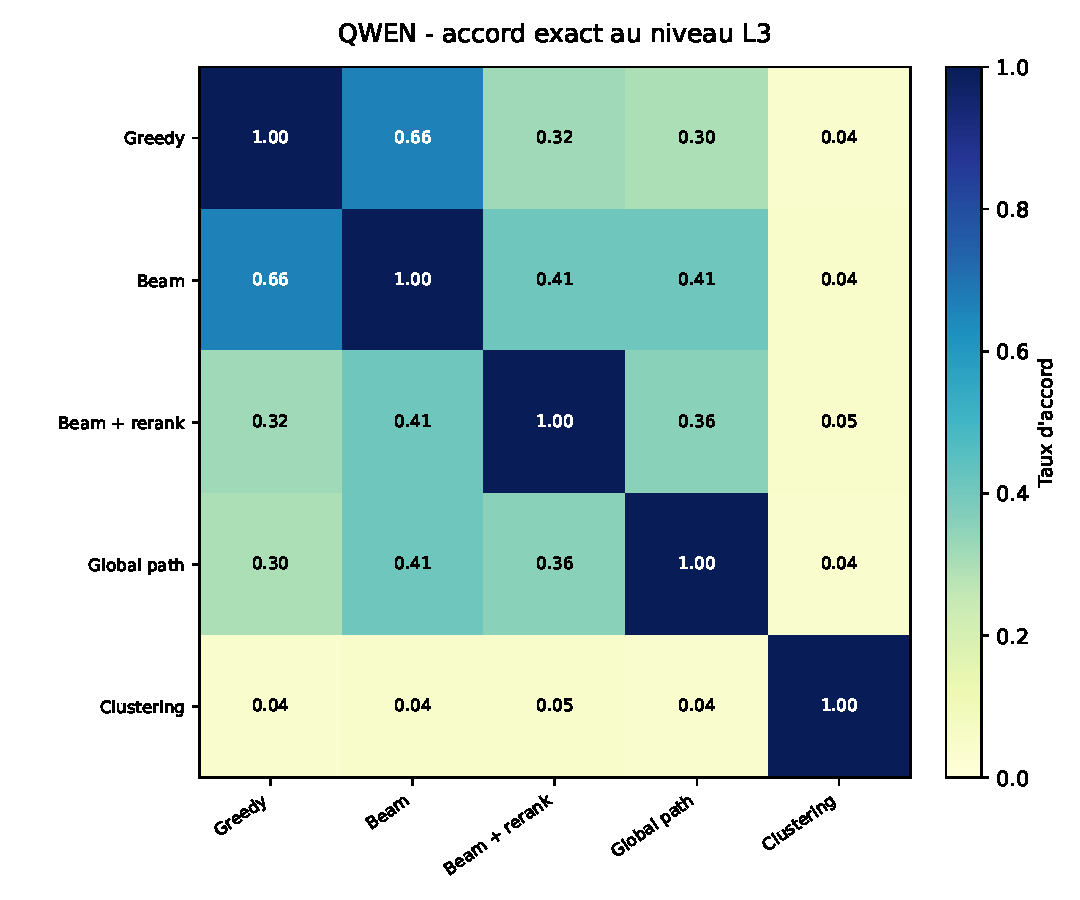
\includegraphics[width=0.48\textwidth]{figures/l2_l7_family3_annex/family3_qwen_level_3_agreement_heatmap.pdf}
    \hfill
    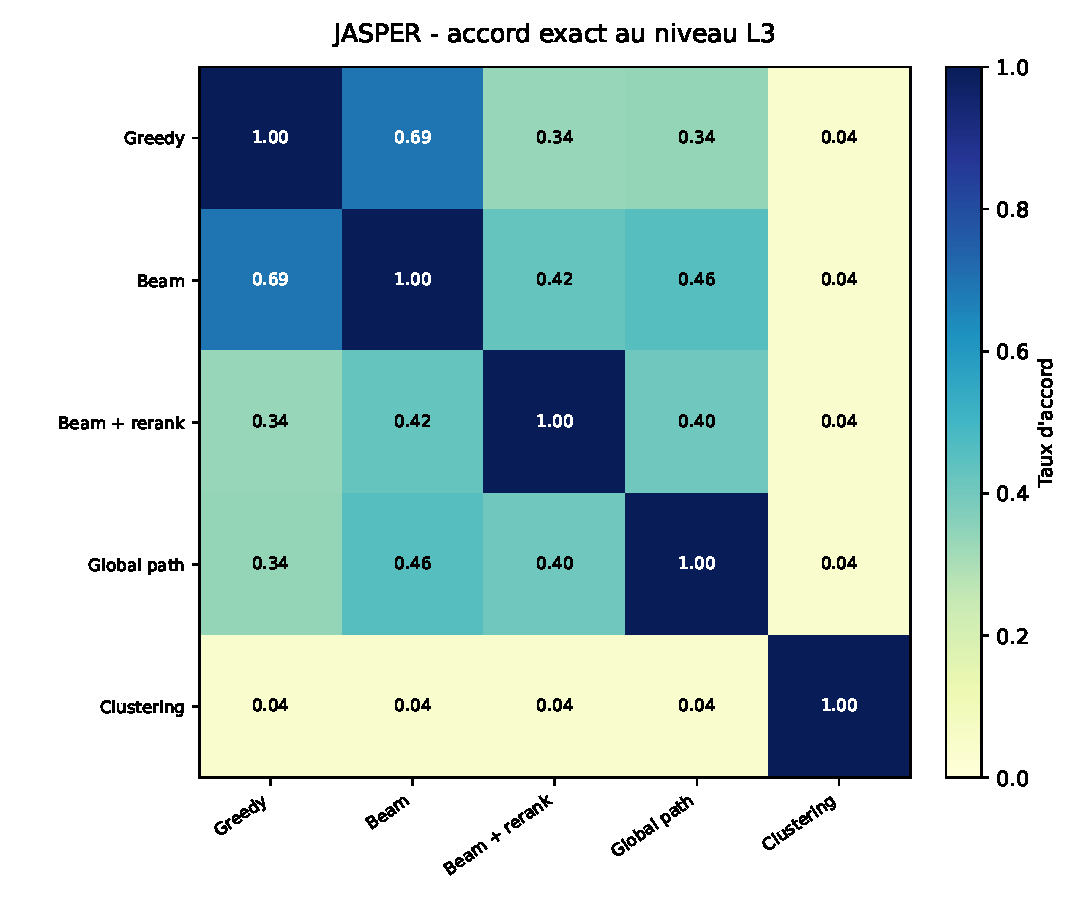
\includegraphics[width=0.48\textwidth]{figures/l2_l7_family3_annex/family3_jasper_level_3_agreement_heatmap.pdf}
    \caption{Matrices d'accord exact au Niveau 3 pour Qwen3, à gauche, et Jasper, à droite.}
    \label{fig:l2-l7-family3-level3-matrix}
\end{figure}

\begin{figure}[H]
    \centering
    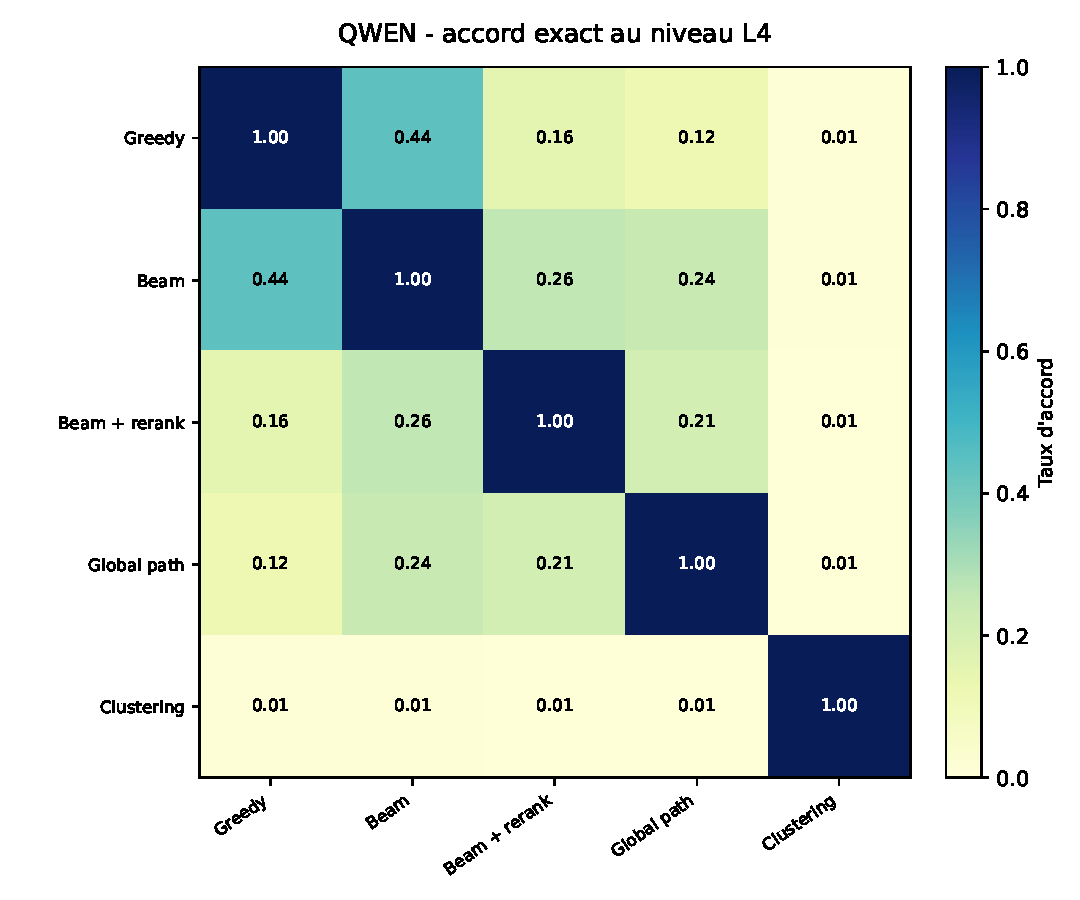
\includegraphics[width=0.48\textwidth]{figures/l2_l7_family3_annex/family3_qwen_level_4_agreement_heatmap.pdf}
    \hfill
    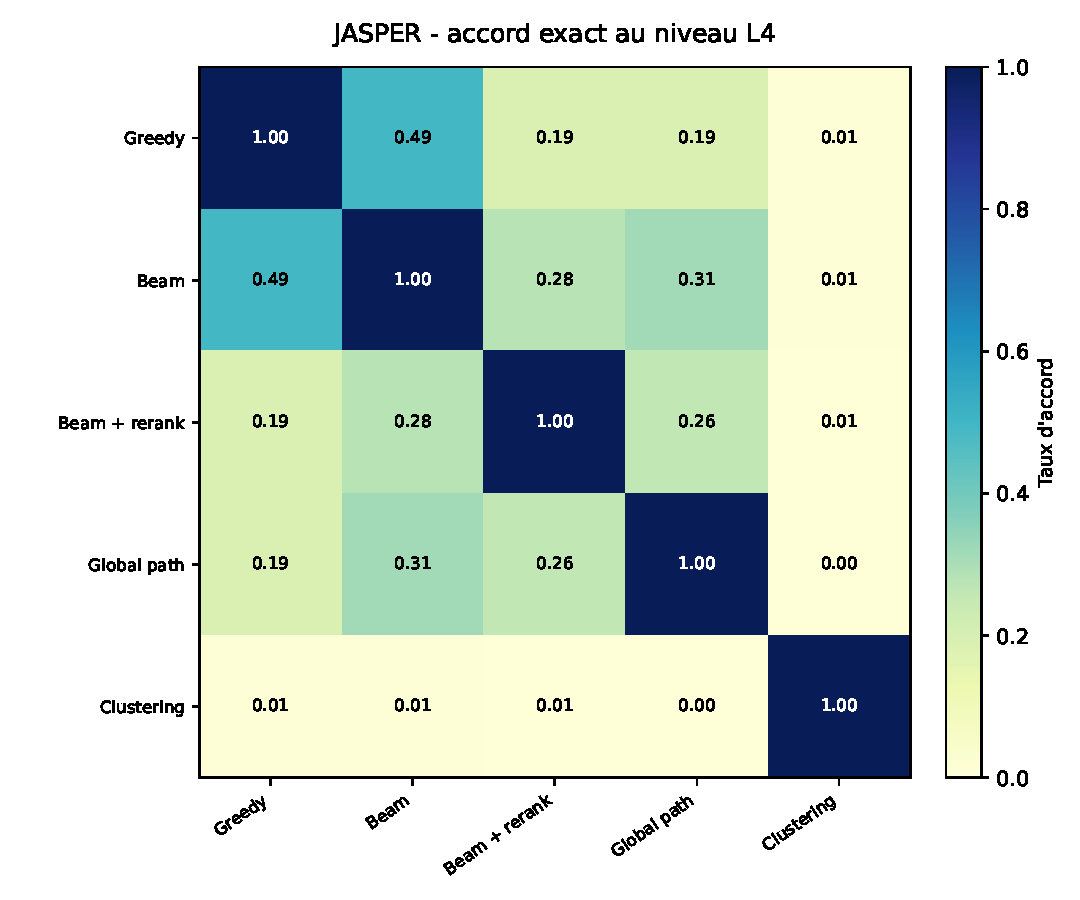
\includegraphics[width=0.48\textwidth]{figures/l2_l7_family3_annex/family3_jasper_level_4_agreement_heatmap.pdf}
    \caption{Matrices d'accord exact au Niveau 4 pour Qwen3, à gauche, et Jasper, à droite.}
    \label{fig:l2-l7-family3-level4-matrix}
\end{figure}

\begin{figure}[H]
    \centering
    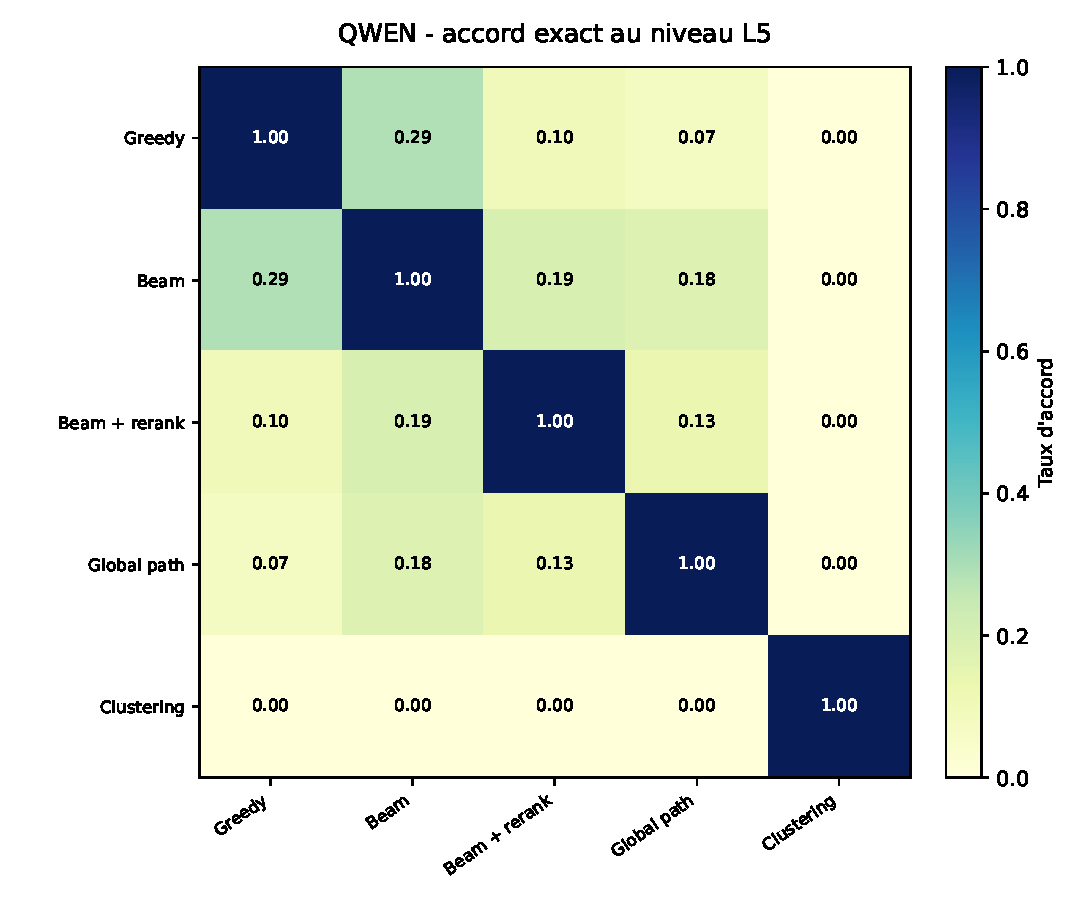
\includegraphics[width=0.48\textwidth]{figures/l2_l7_family3_annex/family3_qwen_level_5_agreement_heatmap.pdf}
    \hfill
    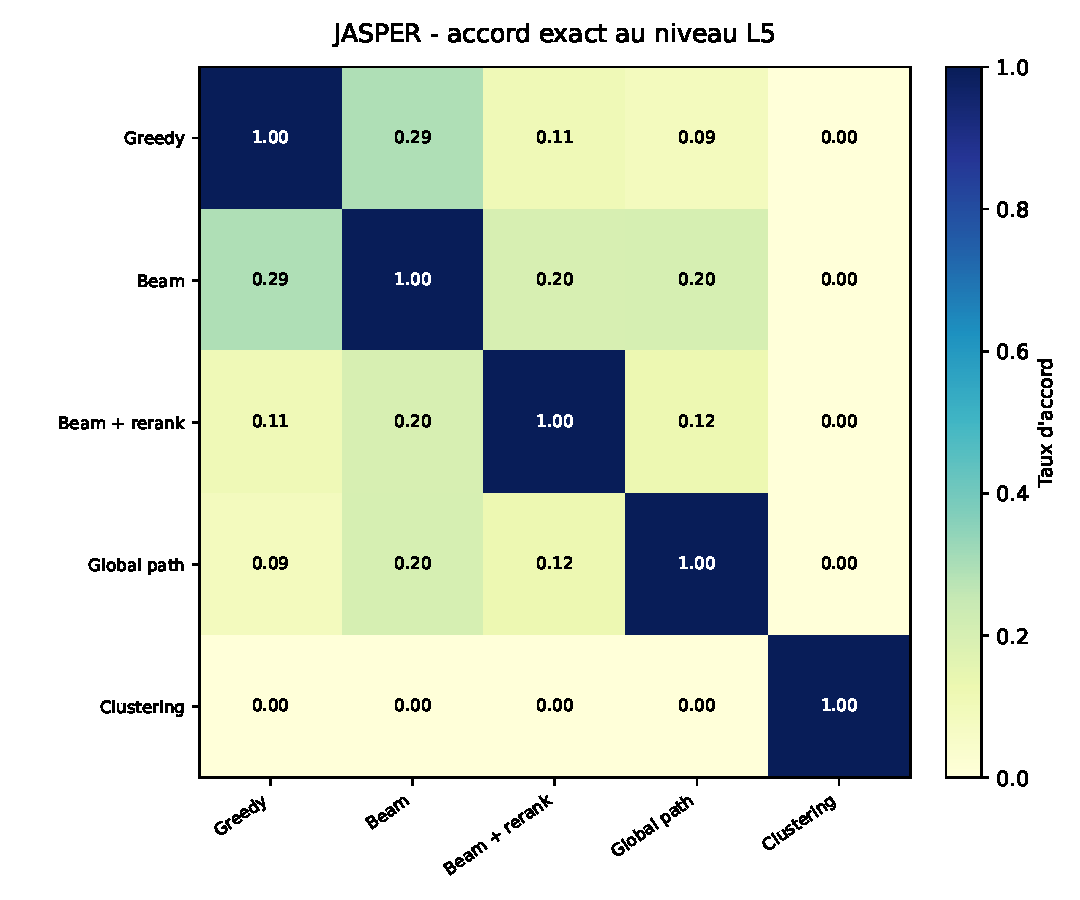
\includegraphics[width=0.48\textwidth]{figures/l2_l7_family3_annex/family3_jasper_level_5_agreement_heatmap.pdf}
    \caption{Matrices d'accord exact au Niveau 5 pour Qwen3, à gauche, et Jasper, à droite.}
    \label{fig:l2-l7-family3-level5-matrix}
\end{figure}

\begin{figure}[H]
    \centering
    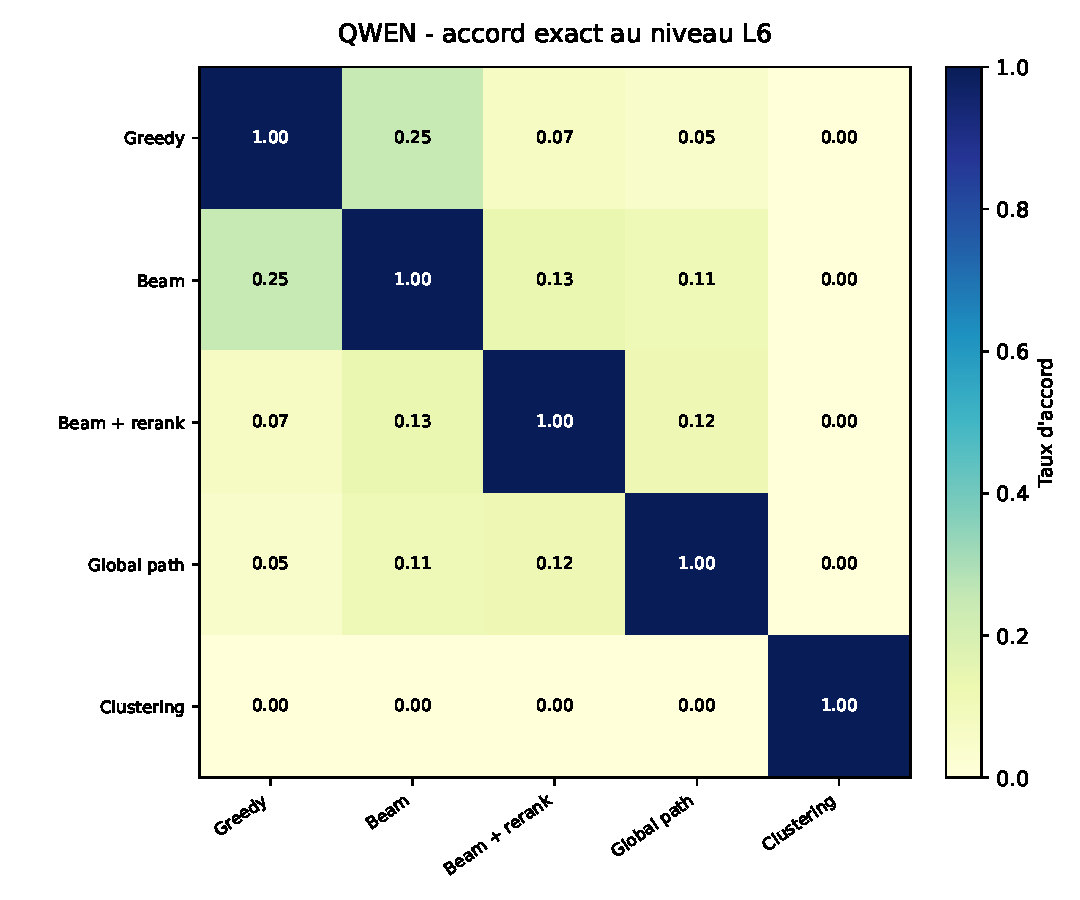
\includegraphics[width=0.48\textwidth]{figures/l2_l7_family3_annex/family3_qwen_level_6_agreement_heatmap.pdf}
    \hfill
    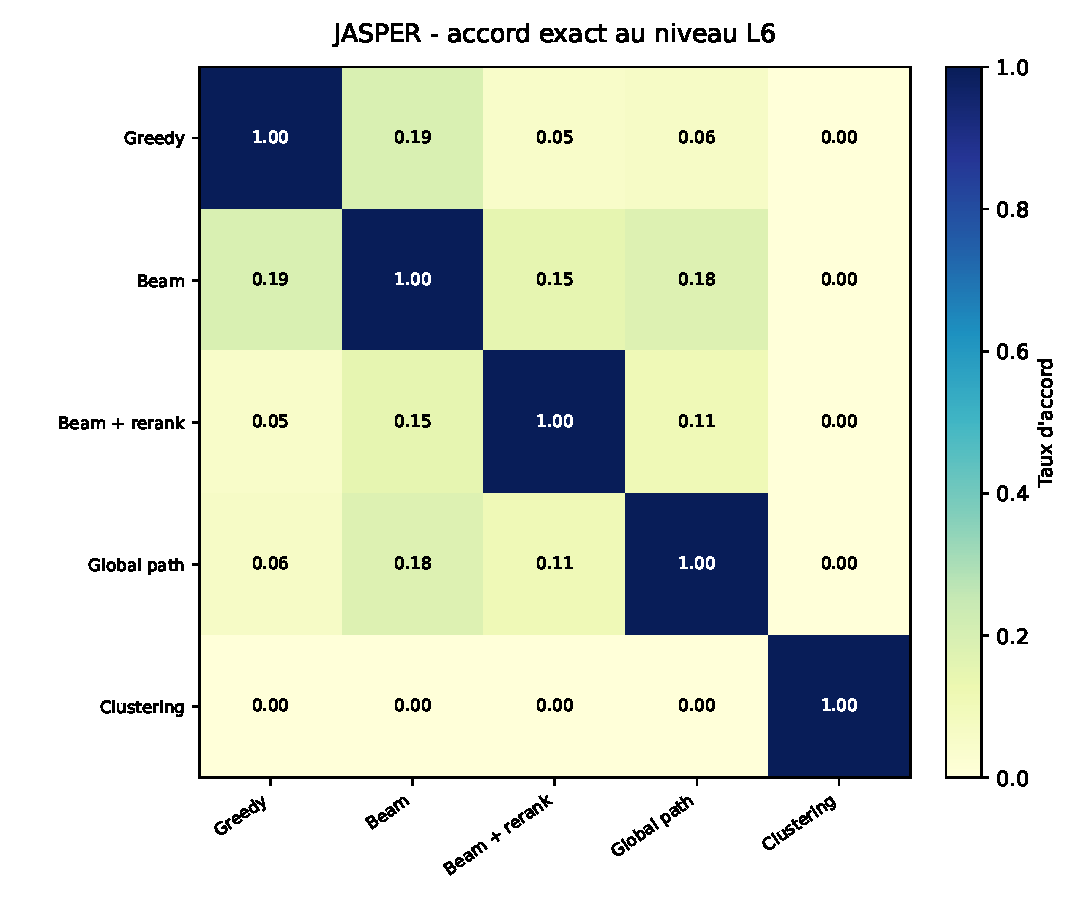
\includegraphics[width=0.48\textwidth]{figures/l2_l7_family3_annex/family3_jasper_level_6_agreement_heatmap.pdf}
    \caption{Matrices d'accord exact au Niveau 6 pour Qwen3, à gauche, et Jasper, à droite.}
    \label{fig:l2-l7-family3-level6-matrix}
\end{figure}

\begin{figure}[H]
    \centering
    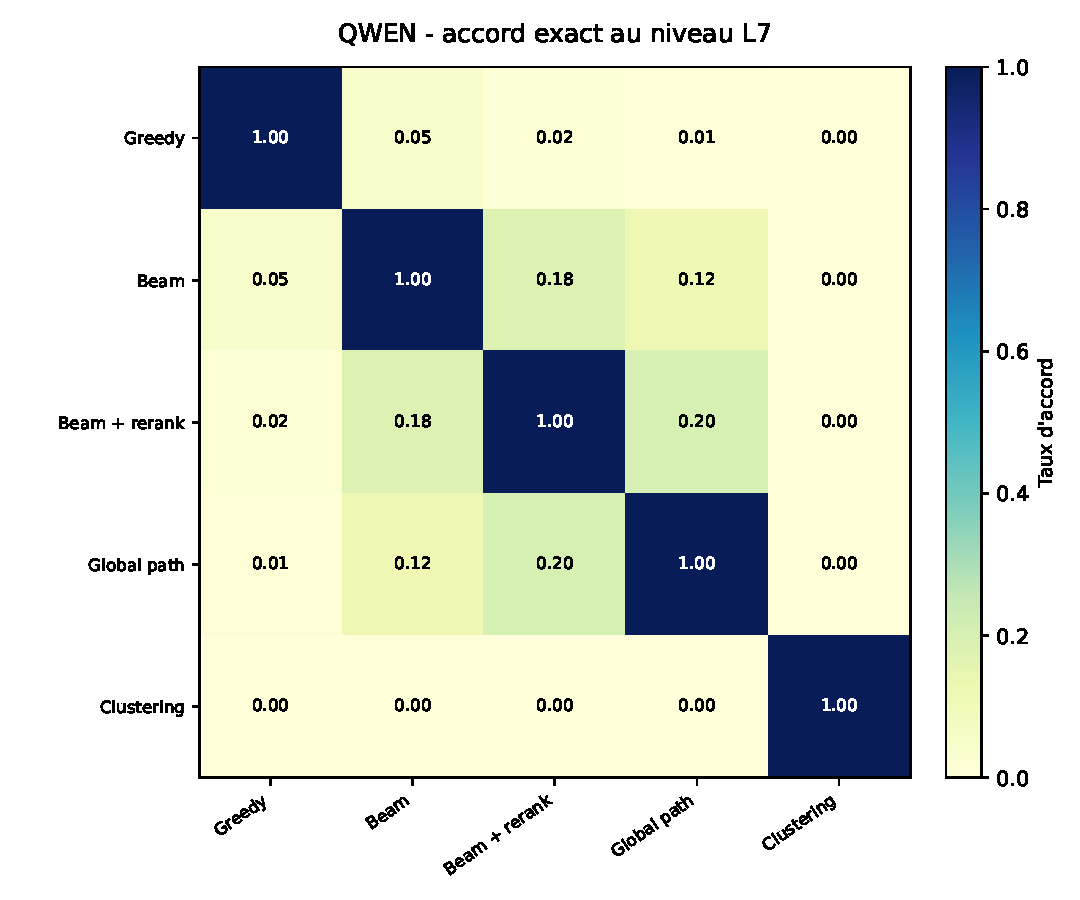
\includegraphics[width=0.48\textwidth]{figures/l2_l7_family3_annex/family3_qwen_level_7_agreement_heatmap.pdf}
    \hfill
    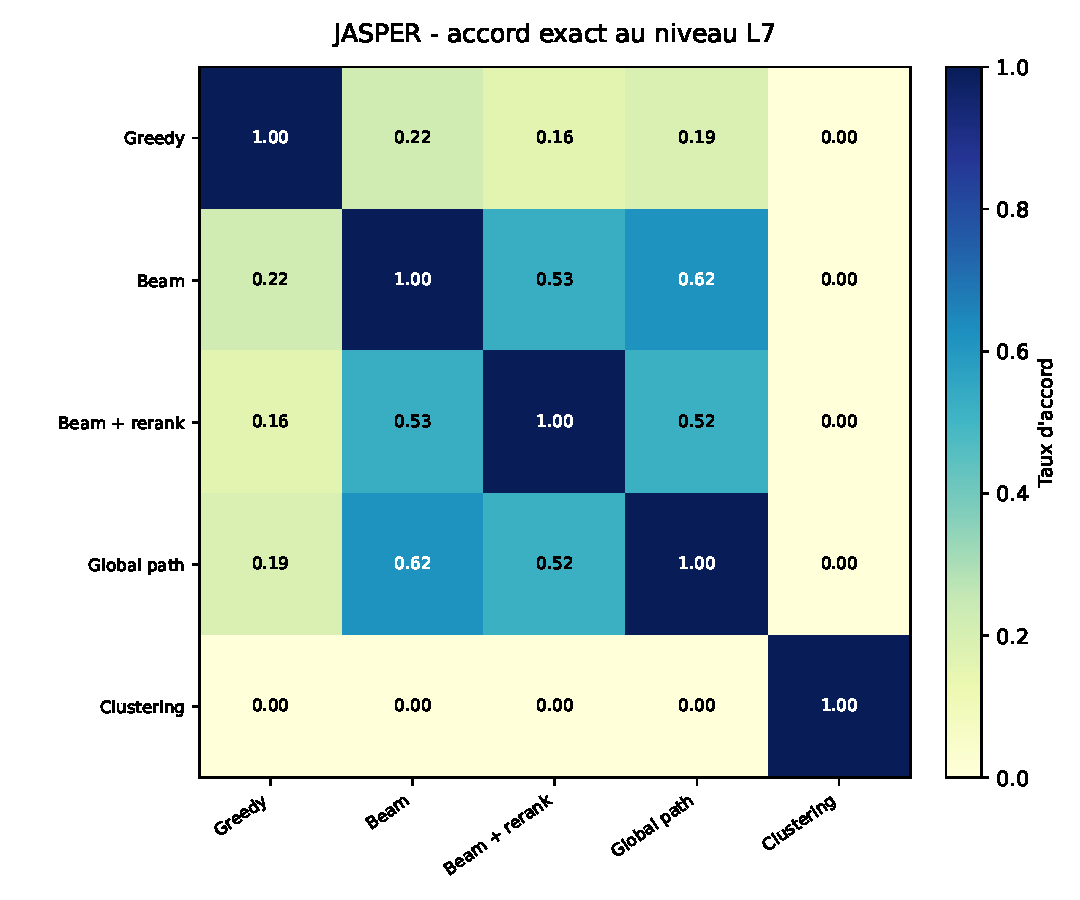
\includegraphics[width=0.48\textwidth]{figures/l2_l7_family3_annex/family3_jasper_level_7_agreement_heatmap.pdf}
    \caption{Matrices d'accord exact au Niveau 7 pour Qwen3, à gauche, et Jasper, à droite.}
    \label{fig:l2-l7-family3-level7-matrix}
\end{figure}

Ces matrices permettent de localiser précisément le niveau où les pipelines divergent. Greedy et beam restent les plus proches sur les premiers niveaux, ce qui confirme que le beam search se comporte comme une extension prudente de la descente greedy. La recherche de chemins globaux conserve une cohérence partielle avec le beam, surtout dans les premiers niveaux, mais diverge davantage à mesure que le chemin devient spécifique. Le clustering est systématiquement le plus éloigné des autres pipelines : cette différence provient de sa logique collective, qui cherche d'abord des groupes de produits avant d'associer ces groupes aux catégories.

\section*{Beam search et reranking pour le décodage hiérarchique}
\label{sec:beam-reranker-annex}

\noindent\hyperref[sec:l2-l7-pipeline-local-decoding]{Retour vers le pipeline de décodage hiérarchique local.}

Cette annexe détaille les deux variantes avancées du pipeline de décodage hiérarchique local : le beam search et le beam search suivi d'un reranker. Ces deux méthodes répondent au même problème : dans une taxonomie profonde, une décision locale incorrecte au Niveau 2 ou au Niveau 3 contraint tous les niveaux suivants. Une descente greedy est donc rapide, mais fragile.

\subsection*{Beam search}

Soit $x$ un produit, $\hat{y}_1$ le Niveau 1 prédit par le modèle fine-tuner, et $u$ un nœud courant de la taxonomie. Pour chaque enfant $c \in \mathrm{Child}(u)$, le score local est :
\begin{equation}
    s(x,c)
    =
    \max_{p \in \mathcal{P}_c}
    \cos\left(g(x),g(p)\right),
\end{equation}
où $g$ est l'encodeur L2--L7 et $\mathcal{P}_c$ l'ensemble des prototypes enrichis de la catégorie $c$.

Un chemin partiel $h=(\hat{y}_1,c_2,\ldots,c_\ell)$ reçoit un score cumulé. Dans notre cas, on utilise une agrégation additive des scores locaux :
\begin{equation}
    S(h \mid x)
    =
    \sum_{t=2}^{\ell} s(x,c_t).
\end{equation}
Une variante possible consiste à normaliser par la longueur du chemin pour éviter de favoriser mécaniquement les chemins profonds :
\begin{equation}
    \bar{S}(h \mid x)
    =
    \frac{1}{\ell-1}
    \sum_{t=2}^{\ell} s(x,c_t).
\end{equation}

L'algorithme conserve à chaque profondeur les $B$ meilleurs chemins partiels. Si $\mathcal{B}_\ell$ désigne le beam à la profondeur $\ell$, l'étape suivante est :
\begin{equation}
    \mathcal{B}_{\ell+1}
    =
    \operatorname{TopB}
    \left\{
    h \oplus c
    \;:\;
    h \in \mathcal{B}_\ell,\ 
    c \in \mathrm{Child}(\mathrm{last}(h))
    \right\}.
\end{equation}
Ici, $h \oplus c$ désigne le chemin obtenu en ajoutant l'enfant $c$ au chemin partiel $h$.

Le beam search est donc un compromis entre greedy et recherche exhaustive. Avec $B=1$, il devient exactement greedy. Lorsque $B$ augmente, il explore plus de branches et peut corriger une décision locale ambiguë en conservant plusieurs hypothèses jusqu'aux niveaux suivants. Son coût augmente cependant avec la largeur du beam et le nombre moyen d'enfants dans la taxonomie. Si $\bar{k}$ est le nombre moyen d'enfants testés par nœud et $D$ la profondeur maximale explorée, le coût est de l'ordre de :
\begin{equation}
    O(B \times \bar{k} \times D)
\end{equation}
comparaisons catégorie--produit par produit, contre $O(\bar{k} \times D)$ pour le greedy.

Dans nos expériences, le beam améliore légèrement la profondeur moyenne prédite par rapport au greedy, mais il conserve souvent une marge top-1/top-2 faible. Cette observation signifie que plusieurs chemins restent plausibles dans l'espace d'embeddings, ce qui justifie l'ajout d'un reranker pour les produits les plus incertains.

\subsection*{Beam search + reranker}

Le reranking intervient après le beam search. Au lieu de choisir directement le chemin ayant le meilleur score cumulé de similarités locales, on conserve les $K$ meilleurs chemins candidats :
\begin{equation}
    \mathcal{H}_K(x)
    =
    \{h_1,\ldots,h_K\}.
\end{equation}
Chaque chemin $h_k$ est transformé en texte, par exemple en concaténant les noms des catégories, le chemin taxonomique et les éléments d'enrichissement associés. Le reranker reçoit alors des couples :
\begin{equation}
    \left(\text{texte produit } x,\ \text{texte du chemin } h_k\right).
\end{equation}

Un modèle de ranking ou un cross-encodeur produit un score global :
\begin{equation}
    r(x,h_k)
    =
    R\left(x,h_k\right).
\end{equation}
La prédiction finale devient :
\begin{equation}
    \hat{h}
    =
    \arg\max_{h_k \in \mathcal{H}_K(x)}
    r(x,h_k).
\end{equation}

L'intérêt du reranker est qu'il évalue le chemin comme une hypothèse globale. Le beam search accumule des décisions locales : un enfant peut être choisi parce qu'il est légèrement meilleur à un niveau donné, même si le chemin complet devient moins cohérent avec le produit. Le reranker corrige ce biais en comparant directement le texte du produit avec la description complète du chemin candidat.

Cette approche a trois avantages. Premièrement, elle réduit le risque de propagation d'erreur, car plusieurs chemins restent disponibles jusqu'à la décision finale. Deuxièmement, elle permet d'utiliser un modèle plus coûteux uniquement sur un petit ensemble de candidats, et non sur toute la taxonomie. Troisièmement, elle produit un score externe utile pour l'audit : si le reranker hésite entre plusieurs chemins, le produit peut être marqué comme incertain.

Sa limite principale est le coût. Si $K$ chemins sont rerankés pour chaque produit, il faut exécuter $K$ évaluations produit--chemin supplémentaires. Le coût devient donc :
\begin{equation}
    C_{\text{beam+rerank}}
    =
    C_{\text{beam}}
    +
    K \cdot C_{\text{reranker}}.
\end{equation}
Dans nos expériences avec Jasper, cette variante atteint 15{,}82 ms par produit, contre 2{,}84 ms pour le beam seul. Elle est donc trop coûteuse pour être appliquée systématiquement si la contrainte principale est la latence, mais elle est pertinente pour les produits à faible marge, les branches ambiguës ou les échantillons destinés à une validation humaine.

Une stratégie opérationnelle naturelle est donc sélective : appliquer greedy ou beam comme méthode standard, puis déclencher le reranker uniquement lorsque la marge top-1/top-2 est inférieure à un seuil $\tau$ :
\begin{equation}
    \Delta(x)
    =
    S(h_1 \mid x) - S(h_2 \mid x)
    <
    \tau.
\end{equation}
Cette règle concentre le coût du reranking sur les produits pour lesquels la décision hiérarchique est réellement incertaine.

\end{document}
